\documentclass[twoside]{book}

% Packages required by doxygen
\usepackage{fixltx2e}
\usepackage{calc}
\usepackage{doxygen}
\usepackage[export]{adjustbox} % also loads graphicx
\usepackage{graphicx}
\usepackage[utf8]{inputenc}
\usepackage{makeidx}
\usepackage{multicol}
\usepackage{multirow}
\PassOptionsToPackage{warn}{textcomp}
\usepackage{textcomp}
\usepackage[nointegrals]{wasysym}
\usepackage[table]{xcolor}

% Font selection
\usepackage[T1]{fontenc}
\usepackage[scaled=.90]{helvet}
\usepackage{courier}
\usepackage{amssymb}
\usepackage{sectsty}
\renewcommand{\familydefault}{\sfdefault}
\allsectionsfont{%
  \fontseries{bc}\selectfont%
  \color{darkgray}%
}
\renewcommand{\DoxyLabelFont}{%
  \fontseries{bc}\selectfont%
  \color{darkgray}%
}
\newcommand{\+}{\discretionary{\mbox{\scriptsize$\hookleftarrow$}}{}{}}

% Page & text layout
\usepackage{geometry}
\geometry{%
  a4paper,%
  top=2.5cm,%
  bottom=2.5cm,%
  left=2.5cm,%
  right=2.5cm%
}
\tolerance=750
\hfuzz=15pt
\hbadness=750
\setlength{\emergencystretch}{15pt}
\setlength{\parindent}{0cm}
\setlength{\parskip}{3ex plus 2ex minus 2ex}
\makeatletter
\renewcommand{\paragraph}{%
  \@startsection{paragraph}{4}{0ex}{-1.0ex}{1.0ex}{%
    \normalfont\normalsize\bfseries\SS@parafont%
  }%
}
\renewcommand{\subparagraph}{%
  \@startsection{subparagraph}{5}{0ex}{-1.0ex}{1.0ex}{%
    \normalfont\normalsize\bfseries\SS@subparafont%
  }%
}
\makeatother

% Headers & footers
\usepackage{fancyhdr}
\pagestyle{fancyplain}
\fancyhead[LE]{\fancyplain{}{\bfseries\thepage}}
\fancyhead[CE]{\fancyplain{}{}}
\fancyhead[RE]{\fancyplain{}{\bfseries\leftmark}}
\fancyhead[LO]{\fancyplain{}{\bfseries\rightmark}}
\fancyhead[CO]{\fancyplain{}{}}
\fancyhead[RO]{\fancyplain{}{\bfseries\thepage}}
\fancyfoot[LE]{\fancyplain{}{}}
\fancyfoot[CE]{\fancyplain{}{}}
\fancyfoot[RE]{\fancyplain{}{\bfseries\scriptsize Generated by Doxygen }}
\fancyfoot[LO]{\fancyplain{}{\bfseries\scriptsize Generated by Doxygen }}
\fancyfoot[CO]{\fancyplain{}{}}
\fancyfoot[RO]{\fancyplain{}{}}
\renewcommand{\footrulewidth}{0.4pt}
\renewcommand{\chaptermark}[1]{%
  \markboth{#1}{}%
}
\renewcommand{\sectionmark}[1]{%
  \markright{\thesection\ #1}%
}

% Indices & bibliography
\usepackage{natbib}
\usepackage[titles]{tocloft}
\setcounter{tocdepth}{3}
\setcounter{secnumdepth}{5}
\makeindex

% Hyperlinks (required, but should be loaded last)
\usepackage{ifpdf}
\ifpdf
  \usepackage[pdftex,pagebackref=true]{hyperref}
\else
  \usepackage[ps2pdf,pagebackref=true]{hyperref}
\fi
\hypersetup{%
  colorlinks=true,%
  linkcolor=blue,%
  citecolor=blue,%
  unicode%
}

% Custom commands
\newcommand{\clearemptydoublepage}{%
  \newpage{\pagestyle{empty}\cleardoublepage}%
}

\usepackage{caption}
\captionsetup{labelsep=space,justification=centering,font={bf},singlelinecheck=off,skip=4pt,position=top}

%===== C O N T E N T S =====

\begin{document}

% Titlepage & ToC
\hypersetup{pageanchor=false,
             bookmarksnumbered=true,
             pdfencoding=unicode
            }
\pagenumbering{roman}
\begin{titlepage}
\vspace*{7cm}
\begin{center}%
{\Large Search }\\
\vspace*{1cm}
{\large Generated by Doxygen 1.8.11}\\
\end{center}
\end{titlepage}
\clearemptydoublepage
\tableofcontents
\clearemptydoublepage
\pagenumbering{arabic}
\hypersetup{pageanchor=true}

%--- Begin generated contents ---
\chapter{R\+E\+A\+D\+ME}
\label{md_README}
\hypertarget{md_README}{}
\href{https://api.travis-ci.org/symbiote-h2020/Search}{\tt } \href{https://codecov.io/github/symbiote-h2020/Search}{\tt }

\section*{Search}
\chapter{Hierarchical Index}
\section{Class Hierarchy}
This inheritance list is sorted roughly, but not completely, alphabetically\+:\begin{DoxyCompactList}
\item \contentsline{section}{eu.\+h2020.\+symbiote.\+ontology.\+model.\+Core\+Information\+Model}{\pageref{classeu_1_1h2020_1_1symbiote_1_1ontology_1_1model_1_1CoreInformationModel}}{}
\item \contentsline{section}{eu.\+h2020.\+symbiote.\+query.\+Delete\+Platform\+Request\+Generator}{\pageref{classeu_1_1h2020_1_1symbiote_1_1query_1_1DeletePlatformRequestGenerator}}{}
\item \contentsline{section}{eu.\+h2020.\+symbiote.\+query.\+Delete\+Resource\+Request\+Generator}{\pageref{classeu_1_1h2020_1_1symbiote_1_1query_1_1DeleteResourceRequestGenerator}}{}
\item \contentsline{section}{eu.\+h2020.\+symbiote.\+handlers.\+Handler\+Utils}{\pageref{classeu_1_1h2020_1_1symbiote_1_1handlers_1_1HandlerUtils}}{}
\item \contentsline{section}{eu.\+h2020.\+symbiote.\+handlers.\+I\+Platform\+Events}{\pageref{interfaceeu_1_1h2020_1_1symbiote_1_1handlers_1_1IPlatformEvents}}{}
\begin{DoxyCompactList}
\item \contentsline{section}{eu.\+h2020.\+symbiote.\+handlers.\+Platform\+Handler}{\pageref{classeu_1_1h2020_1_1symbiote_1_1handlers_1_1PlatformHandler}}{}
\end{DoxyCompactList}
\item \contentsline{section}{eu.\+h2020.\+symbiote.\+handlers.\+I\+Resource\+Delete\+Handler}{\pageref{interfaceeu_1_1h2020_1_1symbiote_1_1handlers_1_1IResourceDeleteHandler}}{}
\item \contentsline{section}{eu.\+h2020.\+symbiote.\+handlers.\+I\+Resource\+Events}{\pageref{interfaceeu_1_1h2020_1_1symbiote_1_1handlers_1_1IResourceEvents}}{}
\begin{DoxyCompactList}
\item \contentsline{section}{eu.\+h2020.\+symbiote.\+handlers.\+Resource\+Handler}{\pageref{classeu_1_1h2020_1_1symbiote_1_1handlers_1_1ResourceHandler}}{}
\end{DoxyCompactList}
\item \contentsline{section}{eu.\+h2020.\+symbiote.\+handlers.\+I\+Search\+Events}{\pageref{interfaceeu_1_1h2020_1_1symbiote_1_1handlers_1_1ISearchEvents}}{}
\begin{DoxyCompactList}
\item \contentsline{section}{eu.\+h2020.\+symbiote.\+handlers.\+Search\+Handler}{\pageref{classeu_1_1h2020_1_1symbiote_1_1handlers_1_1SearchHandler}}{}
\end{DoxyCompactList}
\item \contentsline{section}{eu.\+h2020.\+symbiote.\+model.\+Location}{\pageref{classeu_1_1h2020_1_1symbiote_1_1model_1_1Location}}{}
\item \contentsline{section}{eu.\+h2020.\+symbiote.\+ontology.\+model.\+Meta\+Information\+Model}{\pageref{classeu_1_1h2020_1_1symbiote_1_1ontology_1_1model_1_1MetaInformationModel}}{}
\item \contentsline{section}{eu.\+h2020.\+symbiote.\+ontology.\+model.\+Ontology}{\pageref{classeu_1_1h2020_1_1symbiote_1_1ontology_1_1model_1_1Ontology}}{}
\item \contentsline{section}{eu.\+h2020.\+symbiote.\+model.\+Platform}{\pageref{classeu_1_1h2020_1_1symbiote_1_1model_1_1Platform}}{}
\item \contentsline{section}{eu.\+h2020.\+symbiote.\+query.\+Query\+Generator}{\pageref{classeu_1_1h2020_1_1symbiote_1_1query_1_1QueryGenerator}}{}
\item \contentsline{section}{eu.\+h2020.\+symbiote.\+model.\+Query\+Request}{\pageref{classeu_1_1h2020_1_1symbiote_1_1model_1_1QueryRequest}}{}
\item \contentsline{section}{eu.\+h2020.\+symbiote.\+query.\+Query\+Var\+Name}{\pageref{interfaceeu_1_1h2020_1_1symbiote_1_1query_1_1QueryVarName}}{}
\item \contentsline{section}{eu.\+h2020.\+symbiote.\+communication.\+Rabbit\+Manager}{\pageref{classeu_1_1h2020_1_1symbiote_1_1communication_1_1RabbitManager}}{}
\item \contentsline{section}{eu.\+h2020.\+symbiote.\+ontology.\+model.\+R\+D\+F\+Format}{\pageref{enumeu_1_1h2020_1_1symbiote_1_1ontology_1_1model_1_1RDFFormat}}{}
\item \contentsline{section}{eu.\+h2020.\+symbiote.\+ontology.\+model.\+Registry}{\pageref{classeu_1_1h2020_1_1symbiote_1_1ontology_1_1model_1_1Registry}}{}
\item \contentsline{section}{eu.\+h2020.\+symbiote.\+model.\+Resource}{\pageref{classeu_1_1h2020_1_1symbiote_1_1model_1_1Resource}}{}
\item \contentsline{section}{eu.\+h2020.\+symbiote.\+query.\+Resource\+And\+Observed\+Property\+Query\+Generator}{\pageref{classeu_1_1h2020_1_1symbiote_1_1query_1_1ResourceAndObservedPropertyQueryGenerator}}{}
\item \contentsline{section}{eu.\+h2020.\+symbiote.\+Search\+Application}{\pageref{classeu_1_1h2020_1_1symbiote_1_1SearchApplication}}{}
\item \contentsline{section}{eu.\+h2020.\+symbiote.\+ontology.\+model.\+Search\+Engine}{\pageref{classeu_1_1h2020_1_1symbiote_1_1ontology_1_1model_1_1SearchEngine}}{}
\item \contentsline{section}{eu.\+h2020.\+symbiote.\+query.\+Search\+Request}{\pageref{classeu_1_1h2020_1_1symbiote_1_1query_1_1SearchRequest}}{}
\item \contentsline{section}{eu.\+h2020.\+symbiote.\+query.\+Search\+Response}{\pageref{classeu_1_1h2020_1_1symbiote_1_1query_1_1SearchResponse}}{}
\item \contentsline{section}{eu.\+h2020.\+symbiote.\+query.\+Search\+Response\+Resource}{\pageref{classeu_1_1h2020_1_1symbiote_1_1query_1_1SearchResponseResource}}{}
\item \contentsline{section}{eu.\+h2020.\+symbiote.\+search.\+Search\+Storage}{\pageref{classeu_1_1h2020_1_1symbiote_1_1search_1_1SearchStorage}}{}
\item \contentsline{section}{eu.\+h2020.\+symbiote.\+ontology.\+model.\+Triple\+Store}{\pageref{classeu_1_1h2020_1_1symbiote_1_1ontology_1_1model_1_1TripleStore}}{}
\item \contentsline{section}{eu.\+h2020.\+symbiote.\+query.\+Update\+Platform\+Request\+Generator}{\pageref{classeu_1_1h2020_1_1symbiote_1_1query_1_1UpdatePlatformRequestGenerator}}{}
\item Default\+Consumer\begin{DoxyCompactList}
\item \contentsline{section}{eu.\+h2020.\+symbiote.\+communication.\+Platform\+Created\+Consumer}{\pageref{classeu_1_1h2020_1_1symbiote_1_1communication_1_1PlatformCreatedConsumer}}{}
\item \contentsline{section}{eu.\+h2020.\+symbiote.\+communication.\+Platform\+Deleted\+Consumer}{\pageref{classeu_1_1h2020_1_1symbiote_1_1communication_1_1PlatformDeletedConsumer}}{}
\item \contentsline{section}{eu.\+h2020.\+symbiote.\+communication.\+Platform\+Modified\+Consumer}{\pageref{classeu_1_1h2020_1_1symbiote_1_1communication_1_1PlatformModifiedConsumer}}{}
\item \contentsline{section}{eu.\+h2020.\+symbiote.\+communication.\+Resource\+Created\+Consumer}{\pageref{classeu_1_1h2020_1_1symbiote_1_1communication_1_1ResourceCreatedConsumer}}{}
\item \contentsline{section}{eu.\+h2020.\+symbiote.\+communication.\+Resource\+Deleted\+Consumer}{\pageref{classeu_1_1h2020_1_1symbiote_1_1communication_1_1ResourceDeletedConsumer}}{}
\item \contentsline{section}{eu.\+h2020.\+symbiote.\+communication.\+Resource\+Modified\+Consumer}{\pageref{classeu_1_1h2020_1_1symbiote_1_1communication_1_1ResourceModifiedConsumer}}{}
\item \contentsline{section}{eu.\+h2020.\+symbiote.\+communication.\+Search\+Requested\+Consumer}{\pageref{classeu_1_1h2020_1_1symbiote_1_1communication_1_1SearchRequestedConsumer}}{}
\end{DoxyCompactList}
\end{DoxyCompactList}

\chapter{Class Index}
\section{Class List}
Here are the classes, structs, unions and interfaces with brief descriptions\+:\begin{DoxyCompactList}
\item\contentsline{section}{\hyperlink{classeu_1_1h2020_1_1symbiote_1_1ontology_1_1model_1_1CoreInformationModel}{eu.\+h2020.\+symbiote.\+ontology.\+model.\+Core\+Information\+Model} }{\pageref{classeu_1_1h2020_1_1symbiote_1_1ontology_1_1model_1_1CoreInformationModel}}{}
\item\contentsline{section}{\hyperlink{classeu_1_1h2020_1_1symbiote_1_1query_1_1DeletePlatformRequestGenerator}{eu.\+h2020.\+symbiote.\+query.\+Delete\+Platform\+Request\+Generator} }{\pageref{classeu_1_1h2020_1_1symbiote_1_1query_1_1DeletePlatformRequestGenerator}}{}
\item\contentsline{section}{\hyperlink{classeu_1_1h2020_1_1symbiote_1_1query_1_1DeleteResourceRequestGenerator}{eu.\+h2020.\+symbiote.\+query.\+Delete\+Resource\+Request\+Generator} }{\pageref{classeu_1_1h2020_1_1symbiote_1_1query_1_1DeleteResourceRequestGenerator}}{}
\item\contentsline{section}{\hyperlink{classeu_1_1h2020_1_1symbiote_1_1handlers_1_1HandlerUtils}{eu.\+h2020.\+symbiote.\+handlers.\+Handler\+Utils} }{\pageref{classeu_1_1h2020_1_1symbiote_1_1handlers_1_1HandlerUtils}}{}
\item\contentsline{section}{\hyperlink{interfaceeu_1_1h2020_1_1symbiote_1_1handlers_1_1IPlatformEvents}{eu.\+h2020.\+symbiote.\+handlers.\+I\+Platform\+Events} }{\pageref{interfaceeu_1_1h2020_1_1symbiote_1_1handlers_1_1IPlatformEvents}}{}
\item\contentsline{section}{\hyperlink{interfaceeu_1_1h2020_1_1symbiote_1_1handlers_1_1IResourceDeleteHandler}{eu.\+h2020.\+symbiote.\+handlers.\+I\+Resource\+Delete\+Handler} }{\pageref{interfaceeu_1_1h2020_1_1symbiote_1_1handlers_1_1IResourceDeleteHandler}}{}
\item\contentsline{section}{\hyperlink{interfaceeu_1_1h2020_1_1symbiote_1_1handlers_1_1IResourceEvents}{eu.\+h2020.\+symbiote.\+handlers.\+I\+Resource\+Events} }{\pageref{interfaceeu_1_1h2020_1_1symbiote_1_1handlers_1_1IResourceEvents}}{}
\item\contentsline{section}{\hyperlink{interfaceeu_1_1h2020_1_1symbiote_1_1handlers_1_1ISearchEvents}{eu.\+h2020.\+symbiote.\+handlers.\+I\+Search\+Events} }{\pageref{interfaceeu_1_1h2020_1_1symbiote_1_1handlers_1_1ISearchEvents}}{}
\item\contentsline{section}{\hyperlink{classeu_1_1h2020_1_1symbiote_1_1model_1_1Location}{eu.\+h2020.\+symbiote.\+model.\+Location} }{\pageref{classeu_1_1h2020_1_1symbiote_1_1model_1_1Location}}{}
\item\contentsline{section}{\hyperlink{classeu_1_1h2020_1_1symbiote_1_1ontology_1_1model_1_1MetaInformationModel}{eu.\+h2020.\+symbiote.\+ontology.\+model.\+Meta\+Information\+Model} }{\pageref{classeu_1_1h2020_1_1symbiote_1_1ontology_1_1model_1_1MetaInformationModel}}{}
\item\contentsline{section}{\hyperlink{classeu_1_1h2020_1_1symbiote_1_1ontology_1_1model_1_1Ontology}{eu.\+h2020.\+symbiote.\+ontology.\+model.\+Ontology} }{\pageref{classeu_1_1h2020_1_1symbiote_1_1ontology_1_1model_1_1Ontology}}{}
\item\contentsline{section}{\hyperlink{classeu_1_1h2020_1_1symbiote_1_1model_1_1Platform}{eu.\+h2020.\+symbiote.\+model.\+Platform} }{\pageref{classeu_1_1h2020_1_1symbiote_1_1model_1_1Platform}}{}
\item\contentsline{section}{\hyperlink{classeu_1_1h2020_1_1symbiote_1_1communication_1_1PlatformCreatedConsumer}{eu.\+h2020.\+symbiote.\+communication.\+Platform\+Created\+Consumer} }{\pageref{classeu_1_1h2020_1_1symbiote_1_1communication_1_1PlatformCreatedConsumer}}{}
\item\contentsline{section}{\hyperlink{classeu_1_1h2020_1_1symbiote_1_1communication_1_1PlatformDeletedConsumer}{eu.\+h2020.\+symbiote.\+communication.\+Platform\+Deleted\+Consumer} }{\pageref{classeu_1_1h2020_1_1symbiote_1_1communication_1_1PlatformDeletedConsumer}}{}
\item\contentsline{section}{\hyperlink{classeu_1_1h2020_1_1symbiote_1_1handlers_1_1PlatformHandler}{eu.\+h2020.\+symbiote.\+handlers.\+Platform\+Handler} }{\pageref{classeu_1_1h2020_1_1symbiote_1_1handlers_1_1PlatformHandler}}{}
\item\contentsline{section}{\hyperlink{classeu_1_1h2020_1_1symbiote_1_1communication_1_1PlatformModifiedConsumer}{eu.\+h2020.\+symbiote.\+communication.\+Platform\+Modified\+Consumer} }{\pageref{classeu_1_1h2020_1_1symbiote_1_1communication_1_1PlatformModifiedConsumer}}{}
\item\contentsline{section}{\hyperlink{classeu_1_1h2020_1_1symbiote_1_1query_1_1QueryGenerator}{eu.\+h2020.\+symbiote.\+query.\+Query\+Generator} }{\pageref{classeu_1_1h2020_1_1symbiote_1_1query_1_1QueryGenerator}}{}
\item\contentsline{section}{\hyperlink{classeu_1_1h2020_1_1symbiote_1_1model_1_1QueryRequest}{eu.\+h2020.\+symbiote.\+model.\+Query\+Request} }{\pageref{classeu_1_1h2020_1_1symbiote_1_1model_1_1QueryRequest}}{}
\item\contentsline{section}{\hyperlink{interfaceeu_1_1h2020_1_1symbiote_1_1query_1_1QueryVarName}{eu.\+h2020.\+symbiote.\+query.\+Query\+Var\+Name} }{\pageref{interfaceeu_1_1h2020_1_1symbiote_1_1query_1_1QueryVarName}}{}
\item\contentsline{section}{\hyperlink{classeu_1_1h2020_1_1symbiote_1_1communication_1_1RabbitManager}{eu.\+h2020.\+symbiote.\+communication.\+Rabbit\+Manager} }{\pageref{classeu_1_1h2020_1_1symbiote_1_1communication_1_1RabbitManager}}{}
\item\contentsline{section}{\hyperlink{enumeu_1_1h2020_1_1symbiote_1_1ontology_1_1model_1_1RDFFormat}{eu.\+h2020.\+symbiote.\+ontology.\+model.\+R\+D\+F\+Format} }{\pageref{enumeu_1_1h2020_1_1symbiote_1_1ontology_1_1model_1_1RDFFormat}}{}
\item\contentsline{section}{\hyperlink{classeu_1_1h2020_1_1symbiote_1_1ontology_1_1model_1_1Registry}{eu.\+h2020.\+symbiote.\+ontology.\+model.\+Registry} }{\pageref{classeu_1_1h2020_1_1symbiote_1_1ontology_1_1model_1_1Registry}}{}
\item\contentsline{section}{\hyperlink{classeu_1_1h2020_1_1symbiote_1_1model_1_1Resource}{eu.\+h2020.\+symbiote.\+model.\+Resource} }{\pageref{classeu_1_1h2020_1_1symbiote_1_1model_1_1Resource}}{}
\item\contentsline{section}{\hyperlink{classeu_1_1h2020_1_1symbiote_1_1query_1_1ResourceAndObservedPropertyQueryGenerator}{eu.\+h2020.\+symbiote.\+query.\+Resource\+And\+Observed\+Property\+Query\+Generator} }{\pageref{classeu_1_1h2020_1_1symbiote_1_1query_1_1ResourceAndObservedPropertyQueryGenerator}}{}
\item\contentsline{section}{\hyperlink{classeu_1_1h2020_1_1symbiote_1_1communication_1_1ResourceCreatedConsumer}{eu.\+h2020.\+symbiote.\+communication.\+Resource\+Created\+Consumer} }{\pageref{classeu_1_1h2020_1_1symbiote_1_1communication_1_1ResourceCreatedConsumer}}{}
\item\contentsline{section}{\hyperlink{classeu_1_1h2020_1_1symbiote_1_1communication_1_1ResourceDeletedConsumer}{eu.\+h2020.\+symbiote.\+communication.\+Resource\+Deleted\+Consumer} }{\pageref{classeu_1_1h2020_1_1symbiote_1_1communication_1_1ResourceDeletedConsumer}}{}
\item\contentsline{section}{\hyperlink{classeu_1_1h2020_1_1symbiote_1_1handlers_1_1ResourceHandler}{eu.\+h2020.\+symbiote.\+handlers.\+Resource\+Handler} }{\pageref{classeu_1_1h2020_1_1symbiote_1_1handlers_1_1ResourceHandler}}{}
\item\contentsline{section}{\hyperlink{classeu_1_1h2020_1_1symbiote_1_1communication_1_1ResourceModifiedConsumer}{eu.\+h2020.\+symbiote.\+communication.\+Resource\+Modified\+Consumer} }{\pageref{classeu_1_1h2020_1_1symbiote_1_1communication_1_1ResourceModifiedConsumer}}{}
\item\contentsline{section}{\hyperlink{classeu_1_1h2020_1_1symbiote_1_1SearchApplication}{eu.\+h2020.\+symbiote.\+Search\+Application} }{\pageref{classeu_1_1h2020_1_1symbiote_1_1SearchApplication}}{}
\item\contentsline{section}{\hyperlink{classeu_1_1h2020_1_1symbiote_1_1ontology_1_1model_1_1SearchEngine}{eu.\+h2020.\+symbiote.\+ontology.\+model.\+Search\+Engine} }{\pageref{classeu_1_1h2020_1_1symbiote_1_1ontology_1_1model_1_1SearchEngine}}{}
\item\contentsline{section}{\hyperlink{classeu_1_1h2020_1_1symbiote_1_1handlers_1_1SearchHandler}{eu.\+h2020.\+symbiote.\+handlers.\+Search\+Handler} }{\pageref{classeu_1_1h2020_1_1symbiote_1_1handlers_1_1SearchHandler}}{}
\item\contentsline{section}{\hyperlink{classeu_1_1h2020_1_1symbiote_1_1query_1_1SearchRequest}{eu.\+h2020.\+symbiote.\+query.\+Search\+Request} }{\pageref{classeu_1_1h2020_1_1symbiote_1_1query_1_1SearchRequest}}{}
\item\contentsline{section}{\hyperlink{classeu_1_1h2020_1_1symbiote_1_1communication_1_1SearchRequestedConsumer}{eu.\+h2020.\+symbiote.\+communication.\+Search\+Requested\+Consumer} }{\pageref{classeu_1_1h2020_1_1symbiote_1_1communication_1_1SearchRequestedConsumer}}{}
\item\contentsline{section}{\hyperlink{classeu_1_1h2020_1_1symbiote_1_1query_1_1SearchResponse}{eu.\+h2020.\+symbiote.\+query.\+Search\+Response} }{\pageref{classeu_1_1h2020_1_1symbiote_1_1query_1_1SearchResponse}}{}
\item\contentsline{section}{\hyperlink{classeu_1_1h2020_1_1symbiote_1_1query_1_1SearchResponseResource}{eu.\+h2020.\+symbiote.\+query.\+Search\+Response\+Resource} }{\pageref{classeu_1_1h2020_1_1symbiote_1_1query_1_1SearchResponseResource}}{}
\item\contentsline{section}{\hyperlink{classeu_1_1h2020_1_1symbiote_1_1search_1_1SearchStorage}{eu.\+h2020.\+symbiote.\+search.\+Search\+Storage} }{\pageref{classeu_1_1h2020_1_1symbiote_1_1search_1_1SearchStorage}}{}
\item\contentsline{section}{\hyperlink{classeu_1_1h2020_1_1symbiote_1_1ontology_1_1model_1_1TripleStore}{eu.\+h2020.\+symbiote.\+ontology.\+model.\+Triple\+Store} }{\pageref{classeu_1_1h2020_1_1symbiote_1_1ontology_1_1model_1_1TripleStore}}{}
\item\contentsline{section}{\hyperlink{classeu_1_1h2020_1_1symbiote_1_1query_1_1UpdatePlatformRequestGenerator}{eu.\+h2020.\+symbiote.\+query.\+Update\+Platform\+Request\+Generator} }{\pageref{classeu_1_1h2020_1_1symbiote_1_1query_1_1UpdatePlatformRequestGenerator}}{}
\end{DoxyCompactList}

\chapter{Class Documentation}
\hypertarget{classeu_1_1h2020_1_1symbiote_1_1ontology_1_1model_1_1CoreInformationModel}{}\section{eu.\+h2020.\+symbiote.\+ontology.\+model.\+Core\+Information\+Model Class Reference}
\label{classeu_1_1h2020_1_1symbiote_1_1ontology_1_1model_1_1CoreInformationModel}\index{eu.\+h2020.\+symbiote.\+ontology.\+model.\+Core\+Information\+Model@{eu.\+h2020.\+symbiote.\+ontology.\+model.\+Core\+Information\+Model}}


Collaboration diagram for eu.\+h2020.\+symbiote.\+ontology.\+model.\+Core\+Information\+Model\+:
\nopagebreak
\begin{figure}[H]
\begin{center}
\leavevmode
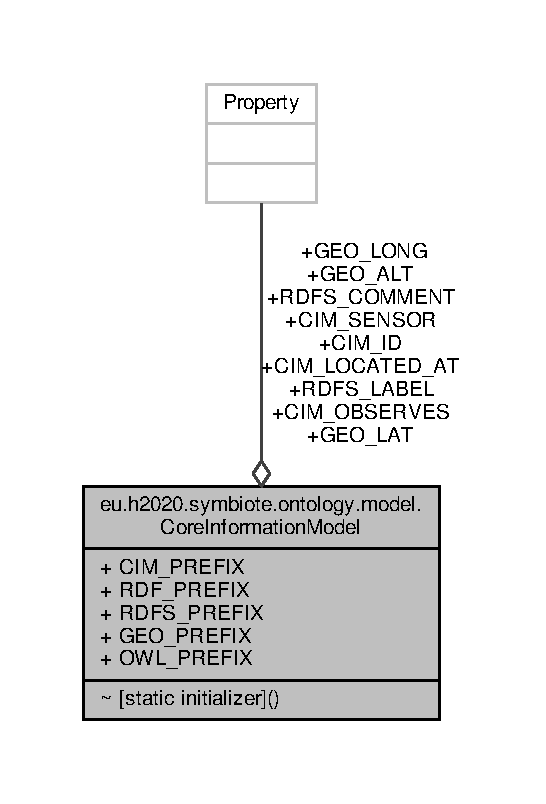
\includegraphics[width=262pt]{classeu_1_1h2020_1_1symbiote_1_1ontology_1_1model_1_1CoreInformationModel__coll__graph}
\end{center}
\end{figure}
\subsection*{Static Public Attributes}
\begin{DoxyCompactItemize}
\item 
static final String {\bfseries C\+I\+M\+\_\+\+P\+R\+E\+F\+IX} = \char`\"{}http\+://www.\+symbiote-\/h2020.\+eu/ontology/core\#\char`\"{}\hypertarget{classeu_1_1h2020_1_1symbiote_1_1ontology_1_1model_1_1CoreInformationModel_a616634a6598159f65ad09d456e9da507}{}\label{classeu_1_1h2020_1_1symbiote_1_1ontology_1_1model_1_1CoreInformationModel_a616634a6598159f65ad09d456e9da507}

\item 
static final String {\bfseries R\+D\+F\+\_\+\+P\+R\+E\+F\+IX} = \char`\"{}http\+://www.\+w3.\+org/1999/02/22-\/rdf-\/syntax-\/ns\#\char`\"{}\hypertarget{classeu_1_1h2020_1_1symbiote_1_1ontology_1_1model_1_1CoreInformationModel_ae03026d29c3d56365d1efc029176b02d}{}\label{classeu_1_1h2020_1_1symbiote_1_1ontology_1_1model_1_1CoreInformationModel_ae03026d29c3d56365d1efc029176b02d}

\item 
static final String {\bfseries R\+D\+F\+S\+\_\+\+P\+R\+E\+F\+IX} = \char`\"{}http\+://www.\+w3.\+org/2000/01/rdf-\/schema\#\char`\"{}\hypertarget{classeu_1_1h2020_1_1symbiote_1_1ontology_1_1model_1_1CoreInformationModel_a1eeee42041f614e80aa328419a7c291f}{}\label{classeu_1_1h2020_1_1symbiote_1_1ontology_1_1model_1_1CoreInformationModel_a1eeee42041f614e80aa328419a7c291f}

\item 
static final String {\bfseries G\+E\+O\+\_\+\+P\+R\+E\+F\+IX} = \char`\"{}http\+://www.\+w3.\+org/2003/01/geo/wgs84\+\_\+pos\#\char`\"{}\hypertarget{classeu_1_1h2020_1_1symbiote_1_1ontology_1_1model_1_1CoreInformationModel_a3d256d6ae2f5cacf2ecdc4e7314f8b06}{}\label{classeu_1_1h2020_1_1symbiote_1_1ontology_1_1model_1_1CoreInformationModel_a3d256d6ae2f5cacf2ecdc4e7314f8b06}

\item 
static final String {\bfseries O\+W\+L\+\_\+\+P\+R\+E\+F\+IX} = \char`\"{}http\+://www.\+w3.\+org/2002/07/owl\#\char`\"{}\hypertarget{classeu_1_1h2020_1_1symbiote_1_1ontology_1_1model_1_1CoreInformationModel_aa358a851fe25eb78ef023e04b9da75e5}{}\label{classeu_1_1h2020_1_1symbiote_1_1ontology_1_1model_1_1CoreInformationModel_aa358a851fe25eb78ef023e04b9da75e5}

\item 
static final Property {\bfseries R\+D\+F\+S\+\_\+\+L\+A\+B\+EL}\hypertarget{classeu_1_1h2020_1_1symbiote_1_1ontology_1_1model_1_1CoreInformationModel_a10f7b98e8a37e005f26b01944ef4d19e}{}\label{classeu_1_1h2020_1_1symbiote_1_1ontology_1_1model_1_1CoreInformationModel_a10f7b98e8a37e005f26b01944ef4d19e}

\item 
static final Property {\bfseries R\+D\+F\+S\+\_\+\+C\+O\+M\+M\+E\+NT}\hypertarget{classeu_1_1h2020_1_1symbiote_1_1ontology_1_1model_1_1CoreInformationModel_a69ec65b7daa64030f03ec60030ffc5fe}{}\label{classeu_1_1h2020_1_1symbiote_1_1ontology_1_1model_1_1CoreInformationModel_a69ec65b7daa64030f03ec60030ffc5fe}

\item 
static final Property {\bfseries C\+I\+M\+\_\+\+S\+E\+N\+S\+OR}\hypertarget{classeu_1_1h2020_1_1symbiote_1_1ontology_1_1model_1_1CoreInformationModel_a32fb89fa0cc2cbfec5a283518d69b68d}{}\label{classeu_1_1h2020_1_1symbiote_1_1ontology_1_1model_1_1CoreInformationModel_a32fb89fa0cc2cbfec5a283518d69b68d}

\item 
static final Property {\bfseries C\+I\+M\+\_\+\+ID}\hypertarget{classeu_1_1h2020_1_1symbiote_1_1ontology_1_1model_1_1CoreInformationModel_acf919bd24eee922a5f1de1e97be7a16f}{}\label{classeu_1_1h2020_1_1symbiote_1_1ontology_1_1model_1_1CoreInformationModel_acf919bd24eee922a5f1de1e97be7a16f}

\item 
static final Property {\bfseries C\+I\+M\+\_\+\+L\+O\+C\+A\+T\+E\+D\+\_\+\+AT}\hypertarget{classeu_1_1h2020_1_1symbiote_1_1ontology_1_1model_1_1CoreInformationModel_a91a1eb308ae8231b01dbb6d38599575f}{}\label{classeu_1_1h2020_1_1symbiote_1_1ontology_1_1model_1_1CoreInformationModel_a91a1eb308ae8231b01dbb6d38599575f}

\item 
static final Property {\bfseries G\+E\+O\+\_\+\+L\+AT}\hypertarget{classeu_1_1h2020_1_1symbiote_1_1ontology_1_1model_1_1CoreInformationModel_a5367bb37684c9a49e32c752852a5f684}{}\label{classeu_1_1h2020_1_1symbiote_1_1ontology_1_1model_1_1CoreInformationModel_a5367bb37684c9a49e32c752852a5f684}

\item 
static final Property {\bfseries G\+E\+O\+\_\+\+L\+O\+NG}\hypertarget{classeu_1_1h2020_1_1symbiote_1_1ontology_1_1model_1_1CoreInformationModel_a066338224786205f688ac7686bbf07a8}{}\label{classeu_1_1h2020_1_1symbiote_1_1ontology_1_1model_1_1CoreInformationModel_a066338224786205f688ac7686bbf07a8}

\item 
static final Property {\bfseries G\+E\+O\+\_\+\+A\+LT}\hypertarget{classeu_1_1h2020_1_1symbiote_1_1ontology_1_1model_1_1CoreInformationModel_ad7c3b4b48b76829c16cb8d3f2b6378ff}{}\label{classeu_1_1h2020_1_1symbiote_1_1ontology_1_1model_1_1CoreInformationModel_ad7c3b4b48b76829c16cb8d3f2b6378ff}

\item 
static final Property {\bfseries C\+I\+M\+\_\+\+O\+B\+S\+E\+R\+V\+ES}\hypertarget{classeu_1_1h2020_1_1symbiote_1_1ontology_1_1model_1_1CoreInformationModel_ab1177e0c2b06f5e2c7d9c9e21e91fdb5}{}\label{classeu_1_1h2020_1_1symbiote_1_1ontology_1_1model_1_1CoreInformationModel_ab1177e0c2b06f5e2c7d9c9e21e91fdb5}

\end{DoxyCompactItemize}


\subsection{Detailed Description}
Contains list of predicates used by symb\+Io\+Te Core Information Model

Created by Mael on 11/01/2017. 

The documentation for this class was generated from the following file\+:\begin{DoxyCompactItemize}
\item 
src/main/java/eu/h2020/symbiote/ontology/model/Core\+Information\+Model.\+java\end{DoxyCompactItemize}

\hypertarget{classeu_1_1h2020_1_1symbiote_1_1query_1_1DeletePlatformRequestGenerator}{}\section{eu.\+h2020.\+symbiote.\+query.\+Delete\+Platform\+Request\+Generator Class Reference}
\label{classeu_1_1h2020_1_1symbiote_1_1query_1_1DeletePlatformRequestGenerator}\index{eu.\+h2020.\+symbiote.\+query.\+Delete\+Platform\+Request\+Generator@{eu.\+h2020.\+symbiote.\+query.\+Delete\+Platform\+Request\+Generator}}


Collaboration diagram for eu.\+h2020.\+symbiote.\+query.\+Delete\+Platform\+Request\+Generator\+:
\nopagebreak
\begin{figure}[H]
\begin{center}
\leavevmode
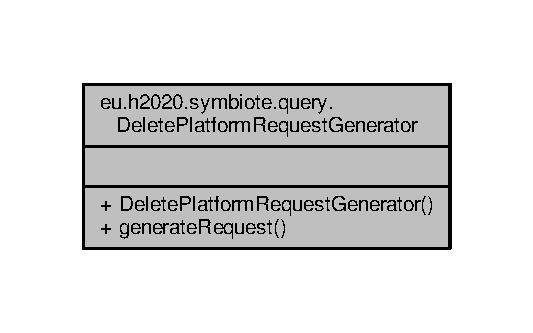
\includegraphics[width=256pt]{classeu_1_1h2020_1_1symbiote_1_1query_1_1DeletePlatformRequestGenerator__coll__graph}
\end{center}
\end{figure}
\subsection*{Public Member Functions}
\begin{DoxyCompactItemize}
\item 
\hyperlink{classeu_1_1h2020_1_1symbiote_1_1query_1_1DeletePlatformRequestGenerator_afa6c0d89bafb8ddb9e99808f758bf9a7}{Delete\+Platform\+Request\+Generator} (String platform\+Id)
\item 
Update\+Request \hyperlink{classeu_1_1h2020_1_1symbiote_1_1query_1_1DeletePlatformRequestGenerator_a1e17c4d72dd0275e9d87de03fbc5df2c}{generate\+Request} ()
\end{DoxyCompactItemize}


\subsection{Detailed Description}
Generator of the delete update operation.

Created by Mael on 26/01/2017. 

\subsection{Constructor \& Destructor Documentation}
\index{eu\+::h2020\+::symbiote\+::query\+::\+Delete\+Platform\+Request\+Generator@{eu\+::h2020\+::symbiote\+::query\+::\+Delete\+Platform\+Request\+Generator}!Delete\+Platform\+Request\+Generator@{Delete\+Platform\+Request\+Generator}}
\index{Delete\+Platform\+Request\+Generator@{Delete\+Platform\+Request\+Generator}!eu\+::h2020\+::symbiote\+::query\+::\+Delete\+Platform\+Request\+Generator@{eu\+::h2020\+::symbiote\+::query\+::\+Delete\+Platform\+Request\+Generator}}
\subsubsection[{\texorpdfstring{Delete\+Platform\+Request\+Generator(\+String platform\+Id)}{DeletePlatformRequestGenerator(String platformId)}}]{\setlength{\rightskip}{0pt plus 5cm}eu.\+h2020.\+symbiote.\+query.\+Delete\+Platform\+Request\+Generator.\+Delete\+Platform\+Request\+Generator (
\begin{DoxyParamCaption}
\item[{String}]{platform\+Id}
\end{DoxyParamCaption}
)}\hypertarget{classeu_1_1h2020_1_1symbiote_1_1query_1_1DeletePlatformRequestGenerator_afa6c0d89bafb8ddb9e99808f758bf9a7}{}\label{classeu_1_1h2020_1_1symbiote_1_1query_1_1DeletePlatformRequestGenerator_afa6c0d89bafb8ddb9e99808f758bf9a7}
Constructor of the delete operation. Prepares S\+P\+A\+R\+QL Update statements to delete the platform with specified id and connected statements. To generate the request use \hyperlink{classeu_1_1h2020_1_1symbiote_1_1query_1_1DeletePlatformRequestGenerator_a1e17c4d72dd0275e9d87de03fbc5df2c}{generate\+Request()}.


\begin{DoxyParams}{Parameters}
{\em platform\+Id} & Id of the resource to be deleted. \\
\hline
\end{DoxyParams}


\subsection{Member Function Documentation}
\index{eu\+::h2020\+::symbiote\+::query\+::\+Delete\+Platform\+Request\+Generator@{eu\+::h2020\+::symbiote\+::query\+::\+Delete\+Platform\+Request\+Generator}!generate\+Request@{generate\+Request}}
\index{generate\+Request@{generate\+Request}!eu\+::h2020\+::symbiote\+::query\+::\+Delete\+Platform\+Request\+Generator@{eu\+::h2020\+::symbiote\+::query\+::\+Delete\+Platform\+Request\+Generator}}
\subsubsection[{\texorpdfstring{generate\+Request()}{generateRequest()}}]{\setlength{\rightskip}{0pt plus 5cm}Update\+Request eu.\+h2020.\+symbiote.\+query.\+Delete\+Platform\+Request\+Generator.\+generate\+Request (
\begin{DoxyParamCaption}
{}
\end{DoxyParamCaption}
)}\hypertarget{classeu_1_1h2020_1_1symbiote_1_1query_1_1DeletePlatformRequestGenerator_a1e17c4d72dd0275e9d87de03fbc5df2c}{}\label{classeu_1_1h2020_1_1symbiote_1_1query_1_1DeletePlatformRequestGenerator_a1e17c4d72dd0275e9d87de03fbc5df2c}
Generates the update request, containing delete queries for resource and data linked to the resource.

\begin{DoxyReturn}{Returns}
Update request which allows deletion of the resource and linked information. 
\end{DoxyReturn}


The documentation for this class was generated from the following file\+:\begin{DoxyCompactItemize}
\item 
src/main/java/eu/h2020/symbiote/query/Delete\+Platform\+Request\+Generator.\+java\end{DoxyCompactItemize}

\hypertarget{classeu_1_1h2020_1_1symbiote_1_1query_1_1DeleteResourceRequestGenerator}{}\section{eu.\+h2020.\+symbiote.\+query.\+Delete\+Resource\+Request\+Generator Class Reference}
\label{classeu_1_1h2020_1_1symbiote_1_1query_1_1DeleteResourceRequestGenerator}\index{eu.\+h2020.\+symbiote.\+query.\+Delete\+Resource\+Request\+Generator@{eu.\+h2020.\+symbiote.\+query.\+Delete\+Resource\+Request\+Generator}}


Collaboration diagram for eu.\+h2020.\+symbiote.\+query.\+Delete\+Resource\+Request\+Generator\+:
\nopagebreak
\begin{figure}[H]
\begin{center}
\leavevmode
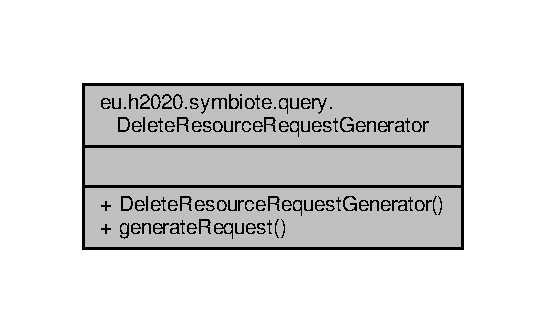
\includegraphics[width=262pt]{classeu_1_1h2020_1_1symbiote_1_1query_1_1DeleteResourceRequestGenerator__coll__graph}
\end{center}
\end{figure}
\subsection*{Public Member Functions}
\begin{DoxyCompactItemize}
\item 
\hyperlink{classeu_1_1h2020_1_1symbiote_1_1query_1_1DeleteResourceRequestGenerator_a60a58d7977ec74141daa2659d56e3166}{Delete\+Resource\+Request\+Generator} (String resource\+Id)
\item 
Update\+Request \hyperlink{classeu_1_1h2020_1_1symbiote_1_1query_1_1DeleteResourceRequestGenerator_a5da00db30549def4d9e17b51011d76b2}{generate\+Request} ()
\end{DoxyCompactItemize}


\subsection{Detailed Description}
Generator of the delete update operation.

Created by Mael on 26/01/2017. 

\subsection{Constructor \& Destructor Documentation}
\index{eu\+::h2020\+::symbiote\+::query\+::\+Delete\+Resource\+Request\+Generator@{eu\+::h2020\+::symbiote\+::query\+::\+Delete\+Resource\+Request\+Generator}!Delete\+Resource\+Request\+Generator@{Delete\+Resource\+Request\+Generator}}
\index{Delete\+Resource\+Request\+Generator@{Delete\+Resource\+Request\+Generator}!eu\+::h2020\+::symbiote\+::query\+::\+Delete\+Resource\+Request\+Generator@{eu\+::h2020\+::symbiote\+::query\+::\+Delete\+Resource\+Request\+Generator}}
\subsubsection[{\texorpdfstring{Delete\+Resource\+Request\+Generator(\+String resource\+Id)}{DeleteResourceRequestGenerator(String resourceId)}}]{\setlength{\rightskip}{0pt plus 5cm}eu.\+h2020.\+symbiote.\+query.\+Delete\+Resource\+Request\+Generator.\+Delete\+Resource\+Request\+Generator (
\begin{DoxyParamCaption}
\item[{String}]{resource\+Id}
\end{DoxyParamCaption}
)}\hypertarget{classeu_1_1h2020_1_1symbiote_1_1query_1_1DeleteResourceRequestGenerator_a60a58d7977ec74141daa2659d56e3166}{}\label{classeu_1_1h2020_1_1symbiote_1_1query_1_1DeleteResourceRequestGenerator_a60a58d7977ec74141daa2659d56e3166}
Constructor of the delete operation. Prepares S\+P\+A\+R\+QL Update statements to delete the resource with specified id, as well as all informations connected to it. To generate the request use \hyperlink{classeu_1_1h2020_1_1symbiote_1_1query_1_1DeleteResourceRequestGenerator_a5da00db30549def4d9e17b51011d76b2}{generate\+Request()}.


\begin{DoxyParams}{Parameters}
{\em resource\+Id} & Id of the resource to be deleted. \\
\hline
\end{DoxyParams}


\subsection{Member Function Documentation}
\index{eu\+::h2020\+::symbiote\+::query\+::\+Delete\+Resource\+Request\+Generator@{eu\+::h2020\+::symbiote\+::query\+::\+Delete\+Resource\+Request\+Generator}!generate\+Request@{generate\+Request}}
\index{generate\+Request@{generate\+Request}!eu\+::h2020\+::symbiote\+::query\+::\+Delete\+Resource\+Request\+Generator@{eu\+::h2020\+::symbiote\+::query\+::\+Delete\+Resource\+Request\+Generator}}
\subsubsection[{\texorpdfstring{generate\+Request()}{generateRequest()}}]{\setlength{\rightskip}{0pt plus 5cm}Update\+Request eu.\+h2020.\+symbiote.\+query.\+Delete\+Resource\+Request\+Generator.\+generate\+Request (
\begin{DoxyParamCaption}
{}
\end{DoxyParamCaption}
)}\hypertarget{classeu_1_1h2020_1_1symbiote_1_1query_1_1DeleteResourceRequestGenerator_a5da00db30549def4d9e17b51011d76b2}{}\label{classeu_1_1h2020_1_1symbiote_1_1query_1_1DeleteResourceRequestGenerator_a5da00db30549def4d9e17b51011d76b2}
Generates the update request, containing delete queries for resource and data linked to the resource.

\begin{DoxyReturn}{Returns}
Update request which allows deletion of the resource and linked information. 
\end{DoxyReturn}


The documentation for this class was generated from the following file\+:\begin{DoxyCompactItemize}
\item 
src/main/java/eu/h2020/symbiote/query/Delete\+Resource\+Request\+Generator.\+java\end{DoxyCompactItemize}

\hypertarget{classeu_1_1h2020_1_1symbiote_1_1handlers_1_1HandlerUtils}{}\section{eu.\+h2020.\+symbiote.\+handlers.\+Handler\+Utils Class Reference}
\label{classeu_1_1h2020_1_1symbiote_1_1handlers_1_1HandlerUtils}\index{eu.\+h2020.\+symbiote.\+handlers.\+Handler\+Utils@{eu.\+h2020.\+symbiote.\+handlers.\+Handler\+Utils}}


Collaboration diagram for eu.\+h2020.\+symbiote.\+handlers.\+Handler\+Utils\+:
\nopagebreak
\begin{figure}[H]
\begin{center}
\leavevmode
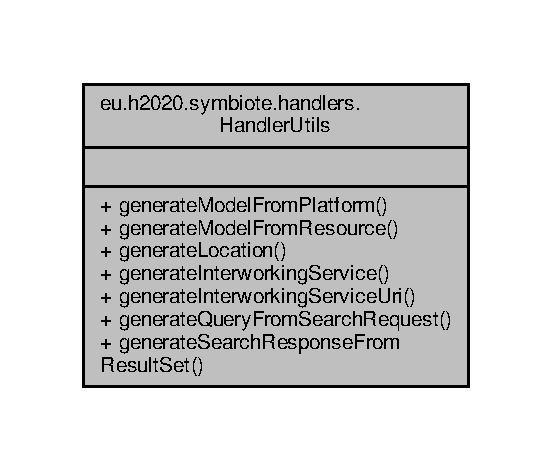
\includegraphics[width=265pt]{classeu_1_1h2020_1_1symbiote_1_1handlers_1_1HandlerUtils__coll__graph}
\end{center}
\end{figure}
\subsection*{Static Public Member Functions}
\begin{DoxyCompactItemize}
\item 
static Model \hyperlink{classeu_1_1h2020_1_1symbiote_1_1handlers_1_1HandlerUtils_ad6758184c042a53b3dbe986b86f7f45f}{generate\+Model\+From\+Platform} (\hyperlink{classeu_1_1h2020_1_1symbiote_1_1model_1_1Platform}{Platform} platform)
\item 
static Model \hyperlink{classeu_1_1h2020_1_1symbiote_1_1handlers_1_1HandlerUtils_a42342da7136ec0aead73f7edde4a77cd}{generate\+Model\+From\+Resource} (\hyperlink{classeu_1_1h2020_1_1symbiote_1_1model_1_1Resource}{Resource} resource)
\item 
static Model \hyperlink{classeu_1_1h2020_1_1symbiote_1_1handlers_1_1HandlerUtils_a909e1a5f76a148cfd82c1b9ba5b1dd91}{generate\+Location} (\hyperlink{classeu_1_1h2020_1_1symbiote_1_1model_1_1Resource}{Resource} resource)
\item 
static Model \hyperlink{classeu_1_1h2020_1_1symbiote_1_1handlers_1_1HandlerUtils_a7fbf9061d7f1d40a19c1257d7d256488}{generate\+Interworking\+Service} (\hyperlink{classeu_1_1h2020_1_1symbiote_1_1model_1_1Platform}{Platform} platform)
\item 
static String \hyperlink{classeu_1_1h2020_1_1symbiote_1_1handlers_1_1HandlerUtils_a292f58eeb374e03ec1591c89b8edced1}{generate\+Interworking\+Service\+Uri} (String platform\+Uri, String service\+Url)
\item 
static \hyperlink{classeu_1_1h2020_1_1symbiote_1_1query_1_1QueryGenerator}{Query\+Generator} \hyperlink{classeu_1_1h2020_1_1symbiote_1_1handlers_1_1HandlerUtils_a0973ccf775f6cbbeed1cc294d8370624}{generate\+Query\+From\+Search\+Request} (\hyperlink{classeu_1_1h2020_1_1symbiote_1_1query_1_1SearchRequest}{Search\+Request} request)
\item 
static \hyperlink{classeu_1_1h2020_1_1symbiote_1_1query_1_1SearchResponse}{Search\+Response} {\bfseries generate\+Search\+Response\+From\+Result\+Set} (Result\+Set result\+Set)\hypertarget{classeu_1_1h2020_1_1symbiote_1_1handlers_1_1HandlerUtils_a64592fa49275e0f94e6865b3da502f95}{}\label{classeu_1_1h2020_1_1symbiote_1_1handlers_1_1HandlerUtils_a64592fa49275e0f94e6865b3da502f95}

\end{DoxyCompactItemize}


\subsection{Detailed Description}
Utility class for translation between event objects and R\+DF models. Contains also some helpers method used by event consumers and executors.

Created by Mael on 12/01/2017. 

\subsection{Member Function Documentation}
\index{eu\+::h2020\+::symbiote\+::handlers\+::\+Handler\+Utils@{eu\+::h2020\+::symbiote\+::handlers\+::\+Handler\+Utils}!generate\+Interworking\+Service@{generate\+Interworking\+Service}}
\index{generate\+Interworking\+Service@{generate\+Interworking\+Service}!eu\+::h2020\+::symbiote\+::handlers\+::\+Handler\+Utils@{eu\+::h2020\+::symbiote\+::handlers\+::\+Handler\+Utils}}
\subsubsection[{\texorpdfstring{generate\+Interworking\+Service(\+Platform platform)}{generateInterworkingService(Platform platform)}}]{\setlength{\rightskip}{0pt plus 5cm}static Model eu.\+h2020.\+symbiote.\+handlers.\+Handler\+Utils.\+generate\+Interworking\+Service (
\begin{DoxyParamCaption}
\item[{{\bf Platform}}]{platform}
\end{DoxyParamCaption}
)\hspace{0.3cm}{\ttfamily [static]}}\hypertarget{classeu_1_1h2020_1_1symbiote_1_1handlers_1_1HandlerUtils_a7fbf9061d7f1d40a19c1257d7d256488}{}\label{classeu_1_1h2020_1_1symbiote_1_1handlers_1_1HandlerUtils_a7fbf9061d7f1d40a19c1257d7d256488}
Generates a model containing R\+DF statements describing interworking service of the specified platform.


\begin{DoxyParams}{Parameters}
{\em platform} & Platform, whose interworking Ssrvice will be translated into R\+DF. \\
\hline
\end{DoxyParams}
\begin{DoxyReturn}{Returns}
Model containing R\+DF statements. 
\end{DoxyReturn}
\index{eu\+::h2020\+::symbiote\+::handlers\+::\+Handler\+Utils@{eu\+::h2020\+::symbiote\+::handlers\+::\+Handler\+Utils}!generate\+Interworking\+Service\+Uri@{generate\+Interworking\+Service\+Uri}}
\index{generate\+Interworking\+Service\+Uri@{generate\+Interworking\+Service\+Uri}!eu\+::h2020\+::symbiote\+::handlers\+::\+Handler\+Utils@{eu\+::h2020\+::symbiote\+::handlers\+::\+Handler\+Utils}}
\subsubsection[{\texorpdfstring{generate\+Interworking\+Service\+Uri(\+String platform\+Uri, String service\+Url)}{generateInterworkingServiceUri(String platformUri, String serviceUrl)}}]{\setlength{\rightskip}{0pt plus 5cm}static String eu.\+h2020.\+symbiote.\+handlers.\+Handler\+Utils.\+generate\+Interworking\+Service\+Uri (
\begin{DoxyParamCaption}
\item[{String}]{platform\+Uri, }
\item[{String}]{service\+Url}
\end{DoxyParamCaption}
)\hspace{0.3cm}{\ttfamily [static]}}\hypertarget{classeu_1_1h2020_1_1symbiote_1_1handlers_1_1HandlerUtils_a292f58eeb374e03ec1591c89b8edced1}{}\label{classeu_1_1h2020_1_1symbiote_1_1handlers_1_1HandlerUtils_a292f58eeb374e03ec1591c89b8edced1}
Generates interworking service uri combining unique platform (graph) U\+RI with service U\+RL of the interwroking service.


\begin{DoxyParams}{Parameters}
{\em platform\+Uri} & Unique graph U\+RI of the platform for which interworking service is created. \\
\hline
{\em service\+Url} & U\+RL of the interworking service. \\
\hline
\end{DoxyParams}
\begin{DoxyReturn}{Returns}
Graph U\+RI of the interworking service. 
\end{DoxyReturn}
\index{eu\+::h2020\+::symbiote\+::handlers\+::\+Handler\+Utils@{eu\+::h2020\+::symbiote\+::handlers\+::\+Handler\+Utils}!generate\+Location@{generate\+Location}}
\index{generate\+Location@{generate\+Location}!eu\+::h2020\+::symbiote\+::handlers\+::\+Handler\+Utils@{eu\+::h2020\+::symbiote\+::handlers\+::\+Handler\+Utils}}
\subsubsection[{\texorpdfstring{generate\+Location(\+Resource resource)}{generateLocation(Resource resource)}}]{\setlength{\rightskip}{0pt plus 5cm}static Model eu.\+h2020.\+symbiote.\+handlers.\+Handler\+Utils.\+generate\+Location (
\begin{DoxyParamCaption}
\item[{{\bf Resource}}]{resource}
\end{DoxyParamCaption}
)\hspace{0.3cm}{\ttfamily [static]}}\hypertarget{classeu_1_1h2020_1_1symbiote_1_1handlers_1_1HandlerUtils_a909e1a5f76a148cfd82c1b9ba5b1dd91}{}\label{classeu_1_1h2020_1_1symbiote_1_1handlers_1_1HandlerUtils_a909e1a5f76a148cfd82c1b9ba5b1dd91}
Generates a model containing R\+DF statements describing resource\textquotesingle{}s location.


\begin{DoxyParams}{Parameters}
{\em resource} & Resource, for which location model will be created. \\
\hline
\end{DoxyParams}
\begin{DoxyReturn}{Returns}
Model containing location R\+DF statements. 
\end{DoxyReturn}
\index{eu\+::h2020\+::symbiote\+::handlers\+::\+Handler\+Utils@{eu\+::h2020\+::symbiote\+::handlers\+::\+Handler\+Utils}!generate\+Model\+From\+Platform@{generate\+Model\+From\+Platform}}
\index{generate\+Model\+From\+Platform@{generate\+Model\+From\+Platform}!eu\+::h2020\+::symbiote\+::handlers\+::\+Handler\+Utils@{eu\+::h2020\+::symbiote\+::handlers\+::\+Handler\+Utils}}
\subsubsection[{\texorpdfstring{generate\+Model\+From\+Platform(\+Platform platform)}{generateModelFromPlatform(Platform platform)}}]{\setlength{\rightskip}{0pt plus 5cm}static Model eu.\+h2020.\+symbiote.\+handlers.\+Handler\+Utils.\+generate\+Model\+From\+Platform (
\begin{DoxyParamCaption}
\item[{{\bf Platform}}]{platform}
\end{DoxyParamCaption}
)\hspace{0.3cm}{\ttfamily [static]}}\hypertarget{classeu_1_1h2020_1_1symbiote_1_1handlers_1_1HandlerUtils_ad6758184c042a53b3dbe986b86f7f45f}{}\label{classeu_1_1h2020_1_1symbiote_1_1handlers_1_1HandlerUtils_ad6758184c042a53b3dbe986b86f7f45f}
Generates a model containing R\+DF statements equivalent to specified platform.


\begin{DoxyParams}{Parameters}
{\em platform} & Platform to be translated into R\+DF. \\
\hline
\end{DoxyParams}
\begin{DoxyReturn}{Returns}
Model containing R\+DF statements. 
\end{DoxyReturn}
\index{eu\+::h2020\+::symbiote\+::handlers\+::\+Handler\+Utils@{eu\+::h2020\+::symbiote\+::handlers\+::\+Handler\+Utils}!generate\+Model\+From\+Resource@{generate\+Model\+From\+Resource}}
\index{generate\+Model\+From\+Resource@{generate\+Model\+From\+Resource}!eu\+::h2020\+::symbiote\+::handlers\+::\+Handler\+Utils@{eu\+::h2020\+::symbiote\+::handlers\+::\+Handler\+Utils}}
\subsubsection[{\texorpdfstring{generate\+Model\+From\+Resource(\+Resource resource)}{generateModelFromResource(Resource resource)}}]{\setlength{\rightskip}{0pt plus 5cm}static Model eu.\+h2020.\+symbiote.\+handlers.\+Handler\+Utils.\+generate\+Model\+From\+Resource (
\begin{DoxyParamCaption}
\item[{{\bf Resource}}]{resource}
\end{DoxyParamCaption}
)\hspace{0.3cm}{\ttfamily [static]}}\hypertarget{classeu_1_1h2020_1_1symbiote_1_1handlers_1_1HandlerUtils_a42342da7136ec0aead73f7edde4a77cd}{}\label{classeu_1_1h2020_1_1symbiote_1_1handlers_1_1HandlerUtils_a42342da7136ec0aead73f7edde4a77cd}
Generates a model containing R\+DF statements equivalent to specified resource.


\begin{DoxyParams}{Parameters}
{\em resource} & Resource to be translated into R\+DF. \\
\hline
\end{DoxyParams}
\begin{DoxyReturn}{Returns}
Model containing R\+DF statements. 
\end{DoxyReturn}
\index{eu\+::h2020\+::symbiote\+::handlers\+::\+Handler\+Utils@{eu\+::h2020\+::symbiote\+::handlers\+::\+Handler\+Utils}!generate\+Query\+From\+Search\+Request@{generate\+Query\+From\+Search\+Request}}
\index{generate\+Query\+From\+Search\+Request@{generate\+Query\+From\+Search\+Request}!eu\+::h2020\+::symbiote\+::handlers\+::\+Handler\+Utils@{eu\+::h2020\+::symbiote\+::handlers\+::\+Handler\+Utils}}
\subsubsection[{\texorpdfstring{generate\+Query\+From\+Search\+Request(\+Search\+Request request)}{generateQueryFromSearchRequest(SearchRequest request)}}]{\setlength{\rightskip}{0pt plus 5cm}static {\bf Query\+Generator} eu.\+h2020.\+symbiote.\+handlers.\+Handler\+Utils.\+generate\+Query\+From\+Search\+Request (
\begin{DoxyParamCaption}
\item[{{\bf Search\+Request}}]{request}
\end{DoxyParamCaption}
)\hspace{0.3cm}{\ttfamily [static]}}\hypertarget{classeu_1_1h2020_1_1symbiote_1_1handlers_1_1HandlerUtils_a0973ccf775f6cbbeed1cc294d8370624}{}\label{classeu_1_1h2020_1_1symbiote_1_1handlers_1_1HandlerUtils_a0973ccf775f6cbbeed1cc294d8370624}

\begin{DoxyParams}{Parameters}
{\em request} & \\
\hline
\end{DoxyParams}
\begin{DoxyReturn}{Returns}

\end{DoxyReturn}


The documentation for this class was generated from the following file\+:\begin{DoxyCompactItemize}
\item 
src/main/java/eu/h2020/symbiote/handlers/Handler\+Utils.\+java\end{DoxyCompactItemize}

\hypertarget{interfaceeu_1_1h2020_1_1symbiote_1_1handlers_1_1IPlatformEvents}{}\section{eu.\+h2020.\+symbiote.\+handlers.\+I\+Platform\+Events Interface Reference}
\label{interfaceeu_1_1h2020_1_1symbiote_1_1handlers_1_1IPlatformEvents}\index{eu.\+h2020.\+symbiote.\+handlers.\+I\+Platform\+Events@{eu.\+h2020.\+symbiote.\+handlers.\+I\+Platform\+Events}}


Inheritance diagram for eu.\+h2020.\+symbiote.\+handlers.\+I\+Platform\+Events\+:
\nopagebreak
\begin{figure}[H]
\begin{center}
\leavevmode
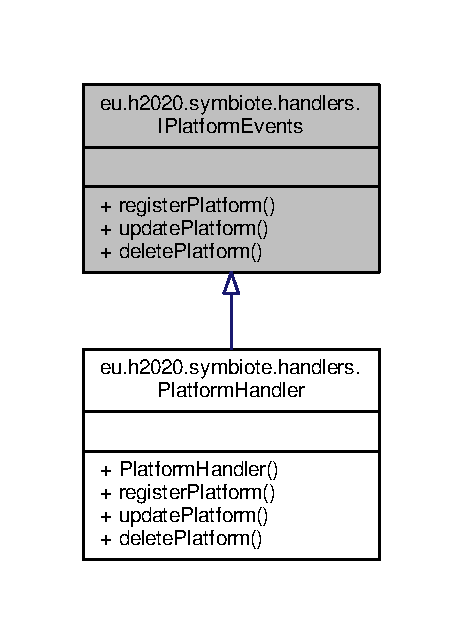
\includegraphics[width=222pt]{interfaceeu_1_1h2020_1_1symbiote_1_1handlers_1_1IPlatformEvents__inherit__graph}
\end{center}
\end{figure}


Collaboration diagram for eu.\+h2020.\+symbiote.\+handlers.\+I\+Platform\+Events\+:
\nopagebreak
\begin{figure}[H]
\begin{center}
\leavevmode
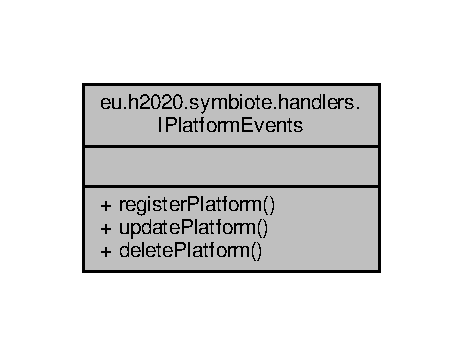
\includegraphics[width=222pt]{interfaceeu_1_1h2020_1_1symbiote_1_1handlers_1_1IPlatformEvents__coll__graph}
\end{center}
\end{figure}
\subsection*{Public Member Functions}
\begin{DoxyCompactItemize}
\item 
boolean \hyperlink{interfaceeu_1_1h2020_1_1symbiote_1_1handlers_1_1IPlatformEvents_a02c6e32eb7af9a13b584a5c911ab8d8c}{register\+Platform} (\hyperlink{classeu_1_1h2020_1_1symbiote_1_1model_1_1Platform}{Platform} platform)
\item 
boolean \hyperlink{interfaceeu_1_1h2020_1_1symbiote_1_1handlers_1_1IPlatformEvents_ad5b491b150e4015525e9985143bbfcd3}{update\+Platform} (\hyperlink{classeu_1_1h2020_1_1symbiote_1_1model_1_1Platform}{Platform} platform)
\item 
boolean \hyperlink{interfaceeu_1_1h2020_1_1symbiote_1_1handlers_1_1IPlatformEvents_aaa59c8d1b1d80f4e58e20227a78c1f23}{delete\+Platform} (String platform\+Id)
\end{DoxyCompactItemize}


\subsection{Detailed Description}
Interface containing all relevant interfaces for Platform related events.

Created by Mael on 11/01/2017. 

\subsection{Member Function Documentation}
\index{eu\+::h2020\+::symbiote\+::handlers\+::\+I\+Platform\+Events@{eu\+::h2020\+::symbiote\+::handlers\+::\+I\+Platform\+Events}!delete\+Platform@{delete\+Platform}}
\index{delete\+Platform@{delete\+Platform}!eu\+::h2020\+::symbiote\+::handlers\+::\+I\+Platform\+Events@{eu\+::h2020\+::symbiote\+::handlers\+::\+I\+Platform\+Events}}
\subsubsection[{\texorpdfstring{delete\+Platform(\+String platform\+Id)}{deletePlatform(String platformId)}}]{\setlength{\rightskip}{0pt plus 5cm}boolean eu.\+h2020.\+symbiote.\+handlers.\+I\+Platform\+Events.\+delete\+Platform (
\begin{DoxyParamCaption}
\item[{String}]{platform\+Id}
\end{DoxyParamCaption}
)}\hypertarget{interfaceeu_1_1h2020_1_1symbiote_1_1handlers_1_1IPlatformEvents_aaa59c8d1b1d80f4e58e20227a78c1f23}{}\label{interfaceeu_1_1h2020_1_1symbiote_1_1handlers_1_1IPlatformEvents_aaa59c8d1b1d80f4e58e20227a78c1f23}
Deletes platform representation in the Apache Jena repository.


\begin{DoxyParams}{Parameters}
{\em platform\+Id} & Id of the platform to be deleted \\
\hline
\end{DoxyParams}
\begin{DoxyReturn}{Returns}
{\ttfamily true} if delete was successful. 
\end{DoxyReturn}


Implemented in \hyperlink{classeu_1_1h2020_1_1symbiote_1_1handlers_1_1PlatformHandler_a3c20ba0a131ad392eb74dd481548a062}{eu.\+h2020.\+symbiote.\+handlers.\+Platform\+Handler}.

\index{eu\+::h2020\+::symbiote\+::handlers\+::\+I\+Platform\+Events@{eu\+::h2020\+::symbiote\+::handlers\+::\+I\+Platform\+Events}!register\+Platform@{register\+Platform}}
\index{register\+Platform@{register\+Platform}!eu\+::h2020\+::symbiote\+::handlers\+::\+I\+Platform\+Events@{eu\+::h2020\+::symbiote\+::handlers\+::\+I\+Platform\+Events}}
\subsubsection[{\texorpdfstring{register\+Platform(\+Platform platform)}{registerPlatform(Platform platform)}}]{\setlength{\rightskip}{0pt plus 5cm}boolean eu.\+h2020.\+symbiote.\+handlers.\+I\+Platform\+Events.\+register\+Platform (
\begin{DoxyParamCaption}
\item[{{\bf Platform}}]{platform}
\end{DoxyParamCaption}
)}\hypertarget{interfaceeu_1_1h2020_1_1symbiote_1_1handlers_1_1IPlatformEvents_a02c6e32eb7af9a13b584a5c911ab8d8c}{}\label{interfaceeu_1_1h2020_1_1symbiote_1_1handlers_1_1IPlatformEvents_a02c6e32eb7af9a13b584a5c911ab8d8c}
Registers platform representation in the Apache Jena repository.


\begin{DoxyParams}{Parameters}
{\em platform} & Platform to be saved \\
\hline
\end{DoxyParams}
\begin{DoxyReturn}{Returns}
{\ttfamily true} if registration was successful. 
\end{DoxyReturn}


Implemented in \hyperlink{classeu_1_1h2020_1_1symbiote_1_1handlers_1_1PlatformHandler_a88a6b019f2d95821ee3f17c8f6c572a9}{eu.\+h2020.\+symbiote.\+handlers.\+Platform\+Handler}.

\index{eu\+::h2020\+::symbiote\+::handlers\+::\+I\+Platform\+Events@{eu\+::h2020\+::symbiote\+::handlers\+::\+I\+Platform\+Events}!update\+Platform@{update\+Platform}}
\index{update\+Platform@{update\+Platform}!eu\+::h2020\+::symbiote\+::handlers\+::\+I\+Platform\+Events@{eu\+::h2020\+::symbiote\+::handlers\+::\+I\+Platform\+Events}}
\subsubsection[{\texorpdfstring{update\+Platform(\+Platform platform)}{updatePlatform(Platform platform)}}]{\setlength{\rightskip}{0pt plus 5cm}boolean eu.\+h2020.\+symbiote.\+handlers.\+I\+Platform\+Events.\+update\+Platform (
\begin{DoxyParamCaption}
\item[{{\bf Platform}}]{platform}
\end{DoxyParamCaption}
)}\hypertarget{interfaceeu_1_1h2020_1_1symbiote_1_1handlers_1_1IPlatformEvents_ad5b491b150e4015525e9985143bbfcd3}{}\label{interfaceeu_1_1h2020_1_1symbiote_1_1handlers_1_1IPlatformEvents_ad5b491b150e4015525e9985143bbfcd3}
Updates platform representation in the Apache Jena repository.


\begin{DoxyParams}{Parameters}
{\em platform} & Platform to be updated \\
\hline
\end{DoxyParams}
\begin{DoxyReturn}{Returns}
{\ttfamily true} if update was successful. 
\end{DoxyReturn}


Implemented in \hyperlink{classeu_1_1h2020_1_1symbiote_1_1handlers_1_1PlatformHandler_ac4701e47973cb2061607dc9ee2916393}{eu.\+h2020.\+symbiote.\+handlers.\+Platform\+Handler}.



The documentation for this interface was generated from the following file\+:\begin{DoxyCompactItemize}
\item 
src/main/java/eu/h2020/symbiote/handlers/I\+Platform\+Events.\+java\end{DoxyCompactItemize}

\hypertarget{interfaceeu_1_1h2020_1_1symbiote_1_1handlers_1_1IResourceDeleteHandler}{}\section{eu.\+h2020.\+symbiote.\+handlers.\+I\+Resource\+Delete\+Handler Interface Reference}
\label{interfaceeu_1_1h2020_1_1symbiote_1_1handlers_1_1IResourceDeleteHandler}\index{eu.\+h2020.\+symbiote.\+handlers.\+I\+Resource\+Delete\+Handler@{eu.\+h2020.\+symbiote.\+handlers.\+I\+Resource\+Delete\+Handler}}


Collaboration diagram for eu.\+h2020.\+symbiote.\+handlers.\+I\+Resource\+Delete\+Handler\+:
\nopagebreak
\begin{figure}[H]
\begin{center}
\leavevmode
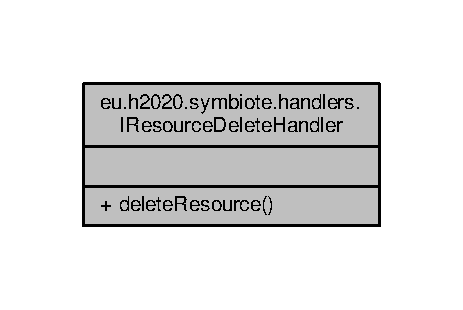
\includegraphics[width=222pt]{interfaceeu_1_1h2020_1_1symbiote_1_1handlers_1_1IResourceDeleteHandler__coll__graph}
\end{center}
\end{figure}
\subsection*{Public Member Functions}
\begin{DoxyCompactItemize}
\item 
void {\bfseries delete\+Resource} (String resource\+Id)\hypertarget{interfaceeu_1_1h2020_1_1symbiote_1_1handlers_1_1IResourceDeleteHandler_a920d821c974799948a8c8afa070a1f73}{}\label{interfaceeu_1_1h2020_1_1symbiote_1_1handlers_1_1IResourceDeleteHandler_a920d821c974799948a8c8afa070a1f73}

\end{DoxyCompactItemize}


\subsection{Detailed Description}
Interface for resource delete events.

Created by Mael on 26/01/2017. 

The documentation for this interface was generated from the following file\+:\begin{DoxyCompactItemize}
\item 
src/main/java/eu/h2020/symbiote/handlers/I\+Resource\+Delete\+Handler.\+java\end{DoxyCompactItemize}

\hypertarget{interfaceeu_1_1h2020_1_1symbiote_1_1handlers_1_1IResourceEvents}{}\section{eu.\+h2020.\+symbiote.\+handlers.\+I\+Resource\+Events Interface Reference}
\label{interfaceeu_1_1h2020_1_1symbiote_1_1handlers_1_1IResourceEvents}\index{eu.\+h2020.\+symbiote.\+handlers.\+I\+Resource\+Events@{eu.\+h2020.\+symbiote.\+handlers.\+I\+Resource\+Events}}


Inheritance diagram for eu.\+h2020.\+symbiote.\+handlers.\+I\+Resource\+Events\+:
\nopagebreak
\begin{figure}[H]
\begin{center}
\leavevmode
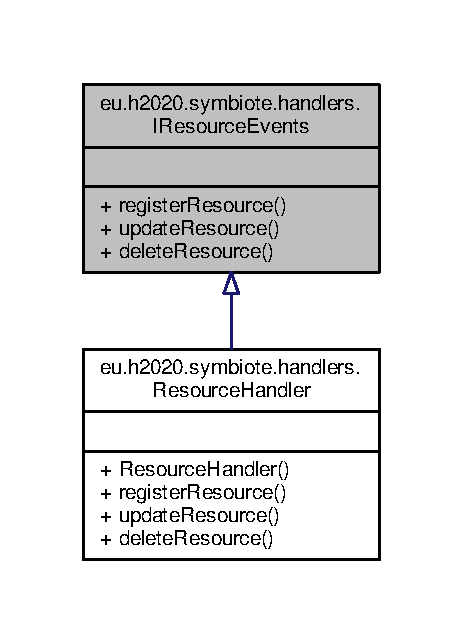
\includegraphics[width=222pt]{interfaceeu_1_1h2020_1_1symbiote_1_1handlers_1_1IResourceEvents__inherit__graph}
\end{center}
\end{figure}


Collaboration diagram for eu.\+h2020.\+symbiote.\+handlers.\+I\+Resource\+Events\+:
\nopagebreak
\begin{figure}[H]
\begin{center}
\leavevmode
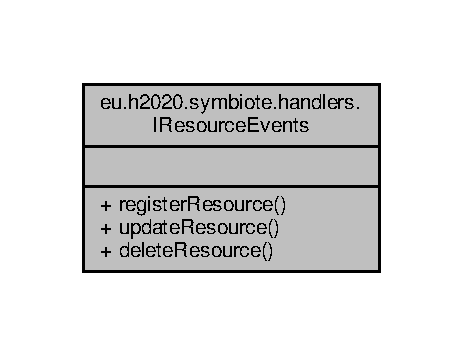
\includegraphics[width=222pt]{interfaceeu_1_1h2020_1_1symbiote_1_1handlers_1_1IResourceEvents__coll__graph}
\end{center}
\end{figure}
\subsection*{Public Member Functions}
\begin{DoxyCompactItemize}
\item 
boolean \hyperlink{interfaceeu_1_1h2020_1_1symbiote_1_1handlers_1_1IResourceEvents_a3941d9229b2efc8d5a80106e0ffe73cd}{register\+Resource} (\hyperlink{classeu_1_1h2020_1_1symbiote_1_1model_1_1Resource}{Resource} resource)
\item 
boolean \hyperlink{interfaceeu_1_1h2020_1_1symbiote_1_1handlers_1_1IResourceEvents_aaac836b0134ed41ad529b9ac3124a216}{update\+Resource} (\hyperlink{classeu_1_1h2020_1_1symbiote_1_1model_1_1Resource}{Resource} resource)
\item 
boolean \hyperlink{interfaceeu_1_1h2020_1_1symbiote_1_1handlers_1_1IResourceEvents_a7c99a8192ec4b06735f641ae3cf2bd99}{delete\+Resource} (String resource\+Id)
\end{DoxyCompactItemize}


\subsection{Detailed Description}
Interface containing all relevant interfaces for Resource related events.

Created by Mael on 16/01/2017. 

\subsection{Member Function Documentation}
\index{eu\+::h2020\+::symbiote\+::handlers\+::\+I\+Resource\+Events@{eu\+::h2020\+::symbiote\+::handlers\+::\+I\+Resource\+Events}!delete\+Resource@{delete\+Resource}}
\index{delete\+Resource@{delete\+Resource}!eu\+::h2020\+::symbiote\+::handlers\+::\+I\+Resource\+Events@{eu\+::h2020\+::symbiote\+::handlers\+::\+I\+Resource\+Events}}
\subsubsection[{\texorpdfstring{delete\+Resource(\+String resource\+Id)}{deleteResource(String resourceId)}}]{\setlength{\rightskip}{0pt plus 5cm}boolean eu.\+h2020.\+symbiote.\+handlers.\+I\+Resource\+Events.\+delete\+Resource (
\begin{DoxyParamCaption}
\item[{String}]{resource\+Id}
\end{DoxyParamCaption}
)}\hypertarget{interfaceeu_1_1h2020_1_1symbiote_1_1handlers_1_1IResourceEvents_a7c99a8192ec4b06735f641ae3cf2bd99}{}\label{interfaceeu_1_1h2020_1_1symbiote_1_1handlers_1_1IResourceEvents_a7c99a8192ec4b06735f641ae3cf2bd99}
Deletes resource representation in the Apache Jena repository.


\begin{DoxyParams}{Parameters}
{\em resource\+Id} & Id of the resource to be deleted \\
\hline
\end{DoxyParams}
\begin{DoxyReturn}{Returns}
{\ttfamily true} if deletion was successful. 
\end{DoxyReturn}


Implemented in \hyperlink{classeu_1_1h2020_1_1symbiote_1_1handlers_1_1ResourceHandler_a549c5bae3e5502b436ba353ba8b39a25}{eu.\+h2020.\+symbiote.\+handlers.\+Resource\+Handler}.

\index{eu\+::h2020\+::symbiote\+::handlers\+::\+I\+Resource\+Events@{eu\+::h2020\+::symbiote\+::handlers\+::\+I\+Resource\+Events}!register\+Resource@{register\+Resource}}
\index{register\+Resource@{register\+Resource}!eu\+::h2020\+::symbiote\+::handlers\+::\+I\+Resource\+Events@{eu\+::h2020\+::symbiote\+::handlers\+::\+I\+Resource\+Events}}
\subsubsection[{\texorpdfstring{register\+Resource(\+Resource resource)}{registerResource(Resource resource)}}]{\setlength{\rightskip}{0pt plus 5cm}boolean eu.\+h2020.\+symbiote.\+handlers.\+I\+Resource\+Events.\+register\+Resource (
\begin{DoxyParamCaption}
\item[{{\bf Resource}}]{resource}
\end{DoxyParamCaption}
)}\hypertarget{interfaceeu_1_1h2020_1_1symbiote_1_1handlers_1_1IResourceEvents_a3941d9229b2efc8d5a80106e0ffe73cd}{}\label{interfaceeu_1_1h2020_1_1symbiote_1_1handlers_1_1IResourceEvents_a3941d9229b2efc8d5a80106e0ffe73cd}
Registers resource representation in the Apache Jena repository.


\begin{DoxyParams}{Parameters}
{\em resource} & Resource to be saved \\
\hline
\end{DoxyParams}
\begin{DoxyReturn}{Returns}
{\ttfamily true} if registration was successful. 
\end{DoxyReturn}


Implemented in \hyperlink{classeu_1_1h2020_1_1symbiote_1_1handlers_1_1ResourceHandler_ab1eb533aab8bcc871ce752edf66ecebd}{eu.\+h2020.\+symbiote.\+handlers.\+Resource\+Handler}.

\index{eu\+::h2020\+::symbiote\+::handlers\+::\+I\+Resource\+Events@{eu\+::h2020\+::symbiote\+::handlers\+::\+I\+Resource\+Events}!update\+Resource@{update\+Resource}}
\index{update\+Resource@{update\+Resource}!eu\+::h2020\+::symbiote\+::handlers\+::\+I\+Resource\+Events@{eu\+::h2020\+::symbiote\+::handlers\+::\+I\+Resource\+Events}}
\subsubsection[{\texorpdfstring{update\+Resource(\+Resource resource)}{updateResource(Resource resource)}}]{\setlength{\rightskip}{0pt plus 5cm}boolean eu.\+h2020.\+symbiote.\+handlers.\+I\+Resource\+Events.\+update\+Resource (
\begin{DoxyParamCaption}
\item[{{\bf Resource}}]{resource}
\end{DoxyParamCaption}
)}\hypertarget{interfaceeu_1_1h2020_1_1symbiote_1_1handlers_1_1IResourceEvents_aaac836b0134ed41ad529b9ac3124a216}{}\label{interfaceeu_1_1h2020_1_1symbiote_1_1handlers_1_1IResourceEvents_aaac836b0134ed41ad529b9ac3124a216}
Updates specified resource representation in the Apache Jena repository.


\begin{DoxyParams}{Parameters}
{\em resource} & Updated resource \\
\hline
\end{DoxyParams}
\begin{DoxyReturn}{Returns}
{\ttfamily true} if update was successful. 
\end{DoxyReturn}


Implemented in \hyperlink{classeu_1_1h2020_1_1symbiote_1_1handlers_1_1ResourceHandler_abeae05c859b45f15b818a6b6640e8ad1}{eu.\+h2020.\+symbiote.\+handlers.\+Resource\+Handler}.



The documentation for this interface was generated from the following file\+:\begin{DoxyCompactItemize}
\item 
src/main/java/eu/h2020/symbiote/handlers/I\+Resource\+Events.\+java\end{DoxyCompactItemize}

\hypertarget{interfaceeu_1_1h2020_1_1symbiote_1_1handlers_1_1ISearchEvents}{}\section{eu.\+h2020.\+symbiote.\+handlers.\+I\+Search\+Events Interface Reference}
\label{interfaceeu_1_1h2020_1_1symbiote_1_1handlers_1_1ISearchEvents}\index{eu.\+h2020.\+symbiote.\+handlers.\+I\+Search\+Events@{eu.\+h2020.\+symbiote.\+handlers.\+I\+Search\+Events}}


Inheritance diagram for eu.\+h2020.\+symbiote.\+handlers.\+I\+Search\+Events\+:
\nopagebreak
\begin{figure}[H]
\begin{center}
\leavevmode
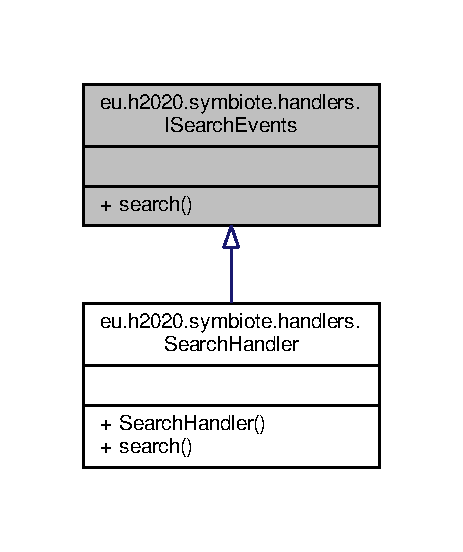
\includegraphics[width=222pt]{interfaceeu_1_1h2020_1_1symbiote_1_1handlers_1_1ISearchEvents__inherit__graph}
\end{center}
\end{figure}


Collaboration diagram for eu.\+h2020.\+symbiote.\+handlers.\+I\+Search\+Events\+:
\nopagebreak
\begin{figure}[H]
\begin{center}
\leavevmode
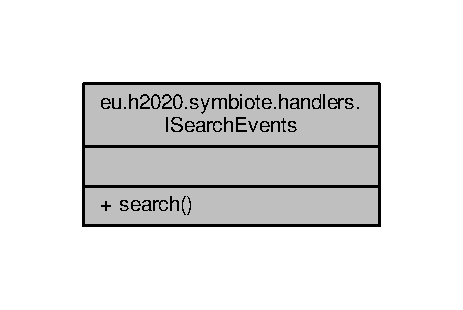
\includegraphics[width=222pt]{interfaceeu_1_1h2020_1_1symbiote_1_1handlers_1_1ISearchEvents__coll__graph}
\end{center}
\end{figure}
\subsection*{Public Member Functions}
\begin{DoxyCompactItemize}
\item 
\hyperlink{classeu_1_1h2020_1_1symbiote_1_1query_1_1SearchResponse}{Search\+Response} \hyperlink{interfaceeu_1_1h2020_1_1symbiote_1_1handlers_1_1ISearchEvents_abbd01c728a329c40370c76d7eea20b12}{search} (\hyperlink{classeu_1_1h2020_1_1symbiote_1_1query_1_1SearchRequest}{Search\+Request} request)
\end{DoxyCompactItemize}


\subsection{Detailed Description}
Interface for handling search events.

Created by Mael on 25/01/2017. 

\subsection{Member Function Documentation}
\index{eu\+::h2020\+::symbiote\+::handlers\+::\+I\+Search\+Events@{eu\+::h2020\+::symbiote\+::handlers\+::\+I\+Search\+Events}!search@{search}}
\index{search@{search}!eu\+::h2020\+::symbiote\+::handlers\+::\+I\+Search\+Events@{eu\+::h2020\+::symbiote\+::handlers\+::\+I\+Search\+Events}}
\subsubsection[{\texorpdfstring{search(\+Search\+Request request)}{search(SearchRequest request)}}]{\setlength{\rightskip}{0pt plus 5cm}{\bf Search\+Response} eu.\+h2020.\+symbiote.\+handlers.\+I\+Search\+Events.\+search (
\begin{DoxyParamCaption}
\item[{{\bf Search\+Request}}]{request}
\end{DoxyParamCaption}
)}\hypertarget{interfaceeu_1_1h2020_1_1symbiote_1_1handlers_1_1ISearchEvents_abbd01c728a329c40370c76d7eea20b12}{}\label{interfaceeu_1_1h2020_1_1symbiote_1_1handlers_1_1ISearchEvents_abbd01c728a329c40370c76d7eea20b12}
Performs search in the module.


\begin{DoxyParams}{Parameters}
{\em request} & Request containing parameters of the search \\
\hline
\end{DoxyParams}
\begin{DoxyReturn}{Returns}
Response containing list of found resources. 
\end{DoxyReturn}


Implemented in \hyperlink{classeu_1_1h2020_1_1symbiote_1_1handlers_1_1SearchHandler_aa1657bbaf89181f753c550f70606ec4c}{eu.\+h2020.\+symbiote.\+handlers.\+Search\+Handler}.



The documentation for this interface was generated from the following file\+:\begin{DoxyCompactItemize}
\item 
src/main/java/eu/h2020/symbiote/handlers/I\+Search\+Events.\+java\end{DoxyCompactItemize}

\hypertarget{classeu_1_1h2020_1_1symbiote_1_1model_1_1Location}{}\section{eu.\+h2020.\+symbiote.\+model.\+Location Class Reference}
\label{classeu_1_1h2020_1_1symbiote_1_1model_1_1Location}\index{eu.\+h2020.\+symbiote.\+model.\+Location@{eu.\+h2020.\+symbiote.\+model.\+Location}}


Collaboration diagram for eu.\+h2020.\+symbiote.\+model.\+Location\+:
\nopagebreak
\begin{figure}[H]
\begin{center}
\leavevmode
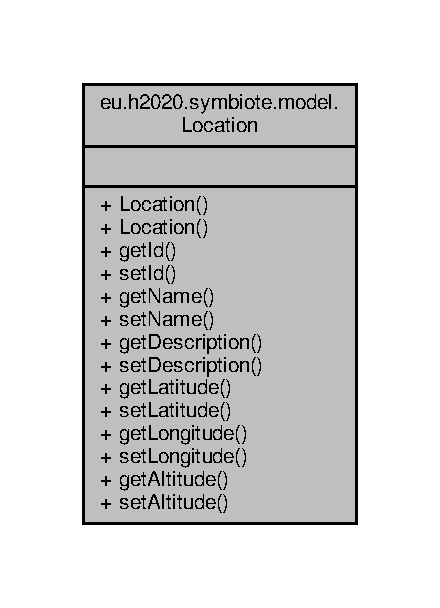
\includegraphics[width=211pt]{classeu_1_1h2020_1_1symbiote_1_1model_1_1Location__coll__graph}
\end{center}
\end{figure}
\subsection*{Public Member Functions}
\begin{DoxyCompactItemize}
\item 
{\bfseries Location} (String id, String name, String description, Double latitude, Double longitude, Double altitude)\hypertarget{classeu_1_1h2020_1_1symbiote_1_1model_1_1Location_a4ea692dd0992307560ce06a254333d3f}{}\label{classeu_1_1h2020_1_1symbiote_1_1model_1_1Location_a4ea692dd0992307560ce06a254333d3f}

\item 
String {\bfseries get\+Id} ()\hypertarget{classeu_1_1h2020_1_1symbiote_1_1model_1_1Location_a98a3b93d177deb7b9630c5e37547d80d}{}\label{classeu_1_1h2020_1_1symbiote_1_1model_1_1Location_a98a3b93d177deb7b9630c5e37547d80d}

\item 
void {\bfseries set\+Id} (String id)\hypertarget{classeu_1_1h2020_1_1symbiote_1_1model_1_1Location_a308f71eeeed57f22b5996da217028d29}{}\label{classeu_1_1h2020_1_1symbiote_1_1model_1_1Location_a308f71eeeed57f22b5996da217028d29}

\item 
String {\bfseries get\+Name} ()\hypertarget{classeu_1_1h2020_1_1symbiote_1_1model_1_1Location_a78e563a2622952f37da6f571932afa23}{}\label{classeu_1_1h2020_1_1symbiote_1_1model_1_1Location_a78e563a2622952f37da6f571932afa23}

\item 
void {\bfseries set\+Name} (String name)\hypertarget{classeu_1_1h2020_1_1symbiote_1_1model_1_1Location_a67ddf61270deeb669ebcdce9b9ead998}{}\label{classeu_1_1h2020_1_1symbiote_1_1model_1_1Location_a67ddf61270deeb669ebcdce9b9ead998}

\item 
String {\bfseries get\+Description} ()\hypertarget{classeu_1_1h2020_1_1symbiote_1_1model_1_1Location_accf0bb0ab10306a962e09fc32c8d821c}{}\label{classeu_1_1h2020_1_1symbiote_1_1model_1_1Location_accf0bb0ab10306a962e09fc32c8d821c}

\item 
void {\bfseries set\+Description} (String description)\hypertarget{classeu_1_1h2020_1_1symbiote_1_1model_1_1Location_a45d3f8f4397791af93669578501a43bf}{}\label{classeu_1_1h2020_1_1symbiote_1_1model_1_1Location_a45d3f8f4397791af93669578501a43bf}

\item 
Double {\bfseries get\+Latitude} ()\hypertarget{classeu_1_1h2020_1_1symbiote_1_1model_1_1Location_af9bf675ed844e386162c04a3ebe18af8}{}\label{classeu_1_1h2020_1_1symbiote_1_1model_1_1Location_af9bf675ed844e386162c04a3ebe18af8}

\item 
void {\bfseries set\+Latitude} (Double latitude)\hypertarget{classeu_1_1h2020_1_1symbiote_1_1model_1_1Location_a316447fb9be5dd5a3ca9afcfdf3c4036}{}\label{classeu_1_1h2020_1_1symbiote_1_1model_1_1Location_a316447fb9be5dd5a3ca9afcfdf3c4036}

\item 
Double {\bfseries get\+Longitude} ()\hypertarget{classeu_1_1h2020_1_1symbiote_1_1model_1_1Location_ab3f74700ec2e761fe77372df1db18ea3}{}\label{classeu_1_1h2020_1_1symbiote_1_1model_1_1Location_ab3f74700ec2e761fe77372df1db18ea3}

\item 
void {\bfseries set\+Longitude} (Double longitude)\hypertarget{classeu_1_1h2020_1_1symbiote_1_1model_1_1Location_afbcdf51fcb5cd1521720f2331ec607fa}{}\label{classeu_1_1h2020_1_1symbiote_1_1model_1_1Location_afbcdf51fcb5cd1521720f2331ec607fa}

\item 
Double {\bfseries get\+Altitude} ()\hypertarget{classeu_1_1h2020_1_1symbiote_1_1model_1_1Location_aa1a73523159adb38828bae17a0cdd1a5}{}\label{classeu_1_1h2020_1_1symbiote_1_1model_1_1Location_aa1a73523159adb38828bae17a0cdd1a5}

\item 
void {\bfseries set\+Altitude} (Double altitude)\hypertarget{classeu_1_1h2020_1_1symbiote_1_1model_1_1Location_a2aed6d3d3fad8ee4a0e5eb06608d3d1d}{}\label{classeu_1_1h2020_1_1symbiote_1_1model_1_1Location_a2aed6d3d3fad8ee4a0e5eb06608d3d1d}

\end{DoxyCompactItemize}


\subsection{Detailed Description}
Class representing W\+G\+S84 geo location in the system events.

Created by Mael on 16/01/2017. 

The documentation for this class was generated from the following file\+:\begin{DoxyCompactItemize}
\item 
src/main/java/eu/h2020/symbiote/model/Location.\+java\end{DoxyCompactItemize}

\hypertarget{classeu_1_1h2020_1_1symbiote_1_1ontology_1_1model_1_1MetaInformationModel}{}\section{eu.\+h2020.\+symbiote.\+ontology.\+model.\+Meta\+Information\+Model Class Reference}
\label{classeu_1_1h2020_1_1symbiote_1_1ontology_1_1model_1_1MetaInformationModel}\index{eu.\+h2020.\+symbiote.\+ontology.\+model.\+Meta\+Information\+Model@{eu.\+h2020.\+symbiote.\+ontology.\+model.\+Meta\+Information\+Model}}


Collaboration diagram for eu.\+h2020.\+symbiote.\+ontology.\+model.\+Meta\+Information\+Model\+:
\nopagebreak
\begin{figure}[H]
\begin{center}
\leavevmode
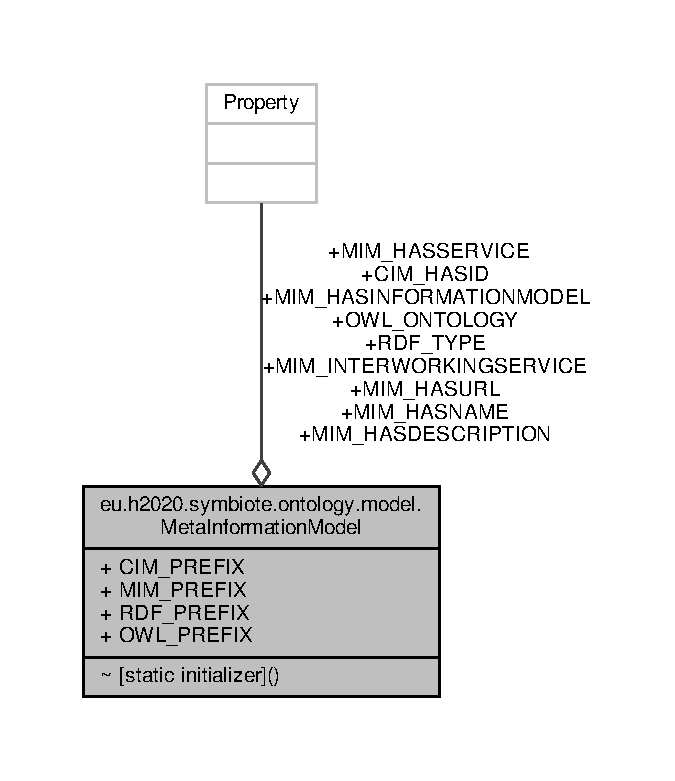
\includegraphics[width=324pt]{classeu_1_1h2020_1_1symbiote_1_1ontology_1_1model_1_1MetaInformationModel__coll__graph}
\end{center}
\end{figure}
\subsection*{Static Public Attributes}
\begin{DoxyCompactItemize}
\item 
static final String {\bfseries C\+I\+M\+\_\+\+P\+R\+E\+F\+IX} = \char`\"{}http\+://www.\+symbiote-\/h2020.\+eu/ontology/core.\+owl\#\char`\"{}\hypertarget{classeu_1_1h2020_1_1symbiote_1_1ontology_1_1model_1_1MetaInformationModel_aa32f19cf912220fe4aca85bee1e8e1d5}{}\label{classeu_1_1h2020_1_1symbiote_1_1ontology_1_1model_1_1MetaInformationModel_aa32f19cf912220fe4aca85bee1e8e1d5}

\item 
static final String {\bfseries M\+I\+M\+\_\+\+P\+R\+E\+F\+IX} = \char`\"{}http\+://www.\+symbiote-\/h2020.\+eu/ontology/meta.\+owl\#\char`\"{}\hypertarget{classeu_1_1h2020_1_1symbiote_1_1ontology_1_1model_1_1MetaInformationModel_a1c8d4b2941c9eadf86b8bcd94d8eda98}{}\label{classeu_1_1h2020_1_1symbiote_1_1ontology_1_1model_1_1MetaInformationModel_a1c8d4b2941c9eadf86b8bcd94d8eda98}

\item 
static final String {\bfseries R\+D\+F\+\_\+\+P\+R\+E\+F\+IX} = \char`\"{}http\+://www.\+w3.\+org/1999/02/22-\/rdf-\/syntax-\/ns\#\char`\"{}\hypertarget{classeu_1_1h2020_1_1symbiote_1_1ontology_1_1model_1_1MetaInformationModel_ab2d07537b5a6830848375bb500eb326b}{}\label{classeu_1_1h2020_1_1symbiote_1_1ontology_1_1model_1_1MetaInformationModel_ab2d07537b5a6830848375bb500eb326b}

\item 
static final String {\bfseries O\+W\+L\+\_\+\+P\+R\+E\+F\+IX} = \char`\"{}http\+://www.\+w3.\+org/2002/07/owl\#\char`\"{}\hypertarget{classeu_1_1h2020_1_1symbiote_1_1ontology_1_1model_1_1MetaInformationModel_a6f74590fdfe17ddf38e81755e0f00731}{}\label{classeu_1_1h2020_1_1symbiote_1_1ontology_1_1model_1_1MetaInformationModel_a6f74590fdfe17ddf38e81755e0f00731}

\item 
static final Property {\bfseries R\+D\+F\+\_\+\+T\+Y\+PE}\hypertarget{classeu_1_1h2020_1_1symbiote_1_1ontology_1_1model_1_1MetaInformationModel_a31dd64c5c10e76fc7b05ec7c38ed8e7b}{}\label{classeu_1_1h2020_1_1symbiote_1_1ontology_1_1model_1_1MetaInformationModel_a31dd64c5c10e76fc7b05ec7c38ed8e7b}

\item 
static final Property {\bfseries O\+W\+L\+\_\+\+O\+N\+T\+O\+L\+O\+GY}\hypertarget{classeu_1_1h2020_1_1symbiote_1_1ontology_1_1model_1_1MetaInformationModel_a223b843d1075d644d50bd9e11873a4b8}{}\label{classeu_1_1h2020_1_1symbiote_1_1ontology_1_1model_1_1MetaInformationModel_a223b843d1075d644d50bd9e11873a4b8}

\item 
static final Property {\bfseries M\+I\+M\+\_\+\+H\+A\+S\+D\+E\+S\+C\+R\+I\+P\+T\+I\+ON}\hypertarget{classeu_1_1h2020_1_1symbiote_1_1ontology_1_1model_1_1MetaInformationModel_adc63b2c36e9ef6d2e4bcea9c1a04f10c}{}\label{classeu_1_1h2020_1_1symbiote_1_1ontology_1_1model_1_1MetaInformationModel_adc63b2c36e9ef6d2e4bcea9c1a04f10c}

\item 
static final Property {\bfseries M\+I\+M\+\_\+\+H\+A\+S\+N\+A\+ME}\hypertarget{classeu_1_1h2020_1_1symbiote_1_1ontology_1_1model_1_1MetaInformationModel_ac551026ed9e01a2370d83e0725f009d8}{}\label{classeu_1_1h2020_1_1symbiote_1_1ontology_1_1model_1_1MetaInformationModel_ac551026ed9e01a2370d83e0725f009d8}

\item 
static final Property {\bfseries M\+I\+M\+\_\+\+H\+A\+S\+S\+E\+R\+V\+I\+CE}\hypertarget{classeu_1_1h2020_1_1symbiote_1_1ontology_1_1model_1_1MetaInformationModel_aed8fdb0a91e8913aeccf8fe104c40a9a}{}\label{classeu_1_1h2020_1_1symbiote_1_1ontology_1_1model_1_1MetaInformationModel_aed8fdb0a91e8913aeccf8fe104c40a9a}

\item 
static final Property {\bfseries M\+I\+M\+\_\+\+H\+A\+S\+I\+N\+F\+O\+R\+M\+A\+T\+I\+O\+N\+M\+O\+D\+EL}\hypertarget{classeu_1_1h2020_1_1symbiote_1_1ontology_1_1model_1_1MetaInformationModel_a4d0155865a5d5bdfb5dab76deebb0e4b}{}\label{classeu_1_1h2020_1_1symbiote_1_1ontology_1_1model_1_1MetaInformationModel_a4d0155865a5d5bdfb5dab76deebb0e4b}

\item 
static final Property {\bfseries C\+I\+M\+\_\+\+H\+A\+S\+ID}\hypertarget{classeu_1_1h2020_1_1symbiote_1_1ontology_1_1model_1_1MetaInformationModel_a1c55281597efb5aa3956dea4bb2c6bec}{}\label{classeu_1_1h2020_1_1symbiote_1_1ontology_1_1model_1_1MetaInformationModel_a1c55281597efb5aa3956dea4bb2c6bec}

\item 
static final Property {\bfseries M\+I\+M\+\_\+\+H\+A\+S\+U\+RL}\hypertarget{classeu_1_1h2020_1_1symbiote_1_1ontology_1_1model_1_1MetaInformationModel_a7b0497cedd88641499e4def59ece5b89}{}\label{classeu_1_1h2020_1_1symbiote_1_1ontology_1_1model_1_1MetaInformationModel_a7b0497cedd88641499e4def59ece5b89}

\item 
static final Property {\bfseries M\+I\+M\+\_\+\+I\+N\+T\+E\+R\+W\+O\+R\+K\+I\+N\+G\+S\+E\+R\+V\+I\+CE}\hypertarget{classeu_1_1h2020_1_1symbiote_1_1ontology_1_1model_1_1MetaInformationModel_aa710605a274a3bd4ba0b57908f6fb48c}{}\label{classeu_1_1h2020_1_1symbiote_1_1ontology_1_1model_1_1MetaInformationModel_aa710605a274a3bd4ba0b57908f6fb48c}

\end{DoxyCompactItemize}


\subsection{Detailed Description}
Contains list of predicates used by symb\+Io\+Te Metainformation Model

Created by Mael on 11/01/2017. 

The documentation for this class was generated from the following file\+:\begin{DoxyCompactItemize}
\item 
src/main/java/eu/h2020/symbiote/ontology/model/Meta\+Information\+Model.\+java\end{DoxyCompactItemize}

\hypertarget{classeu_1_1h2020_1_1symbiote_1_1ontology_1_1model_1_1Ontology}{}\section{eu.\+h2020.\+symbiote.\+ontology.\+model.\+Ontology Class Reference}
\label{classeu_1_1h2020_1_1symbiote_1_1ontology_1_1model_1_1Ontology}\index{eu.\+h2020.\+symbiote.\+ontology.\+model.\+Ontology@{eu.\+h2020.\+symbiote.\+ontology.\+model.\+Ontology}}


Collaboration diagram for eu.\+h2020.\+symbiote.\+ontology.\+model.\+Ontology\+:
\nopagebreak
\begin{figure}[H]
\begin{center}
\leavevmode
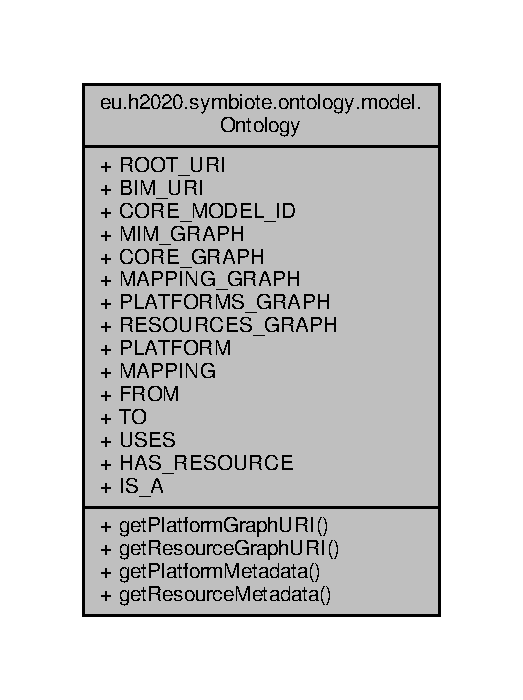
\includegraphics[width=251pt]{classeu_1_1h2020_1_1symbiote_1_1ontology_1_1model_1_1Ontology__coll__graph}
\end{center}
\end{figure}
\subsection*{Static Public Member Functions}
\begin{DoxyCompactItemize}
\item 
static String {\bfseries get\+Platform\+Graph\+U\+RI} (String platform\+Id)\hypertarget{classeu_1_1h2020_1_1symbiote_1_1ontology_1_1model_1_1Ontology_aa76aa8cf3ce95ab4e6d7ba8a7e716aef}{}\label{classeu_1_1h2020_1_1symbiote_1_1ontology_1_1model_1_1Ontology_aa76aa8cf3ce95ab4e6d7ba8a7e716aef}

\item 
static String {\bfseries get\+Resource\+Graph\+U\+RI} (String resource\+Id)\hypertarget{classeu_1_1h2020_1_1symbiote_1_1ontology_1_1model_1_1Ontology_a986882538f6fea21309f7334418d17dc}{}\label{classeu_1_1h2020_1_1symbiote_1_1ontology_1_1model_1_1Ontology_a986882538f6fea21309f7334418d17dc}

\item 
static String {\bfseries get\+Platform\+Metadata} (String platform\+Id, String model\+Id)\hypertarget{classeu_1_1h2020_1_1symbiote_1_1ontology_1_1model_1_1Ontology_a9c5bddffb57bbae8395a2ac9059f8475}{}\label{classeu_1_1h2020_1_1symbiote_1_1ontology_1_1model_1_1Ontology_a9c5bddffb57bbae8395a2ac9059f8475}

\item 
static String {\bfseries get\+Resource\+Metadata} (String service\+U\+RI, String resource\+Uri)\hypertarget{classeu_1_1h2020_1_1symbiote_1_1ontology_1_1model_1_1Ontology_a34a0c58bdf9fa8f3d7b3f95124e9a97f}{}\label{classeu_1_1h2020_1_1symbiote_1_1ontology_1_1model_1_1Ontology_a34a0c58bdf9fa8f3d7b3f95124e9a97f}

\end{DoxyCompactItemize}
\subsection*{Static Public Attributes}
\begin{DoxyCompactItemize}
\item 
static final String {\bfseries R\+O\+O\+T\+\_\+\+U\+RI} = \char`\"{}http\+://www.\+symbiote-\/h2020.\+eu/ontology/\char`\"{}\hypertarget{classeu_1_1h2020_1_1symbiote_1_1ontology_1_1model_1_1Ontology_ad4ba69ae7dac12c22d8ef04eb601e58a}{}\label{classeu_1_1h2020_1_1symbiote_1_1ontology_1_1model_1_1Ontology_ad4ba69ae7dac12c22d8ef04eb601e58a}

\item 
static final String {\bfseries B\+I\+M\+\_\+\+U\+RI} = R\+O\+O\+T\+\_\+\+U\+RI + \char`\"{}bim\char`\"{}\hypertarget{classeu_1_1h2020_1_1symbiote_1_1ontology_1_1model_1_1Ontology_a7aaa930fb8161880239a7ac52f216225}{}\label{classeu_1_1h2020_1_1symbiote_1_1ontology_1_1model_1_1Ontology_a7aaa930fb8161880239a7ac52f216225}

\item 
static final int {\bfseries C\+O\+R\+E\+\_\+\+M\+O\+D\+E\+L\+\_\+\+ID} = -\/1\hypertarget{classeu_1_1h2020_1_1symbiote_1_1ontology_1_1model_1_1Ontology_aa5544a19fc902c62fbbab535b9d5fd25}{}\label{classeu_1_1h2020_1_1symbiote_1_1ontology_1_1model_1_1Ontology_aa5544a19fc902c62fbbab535b9d5fd25}

\item 
static final String \hyperlink{classeu_1_1h2020_1_1symbiote_1_1ontology_1_1model_1_1Ontology_abd334d1878740c80789fc2c6a9bf8afe}{M\+I\+M\+\_\+\+G\+R\+A\+PH} = R\+O\+O\+T\+\_\+\+U\+RI + \char`\"{}meta.\+owl\char`\"{}
\item 
static final String {\bfseries C\+O\+R\+E\+\_\+\+G\+R\+A\+PH} = R\+O\+O\+T\+\_\+\+U\+RI + \char`\"{}core\char`\"{}\hypertarget{classeu_1_1h2020_1_1symbiote_1_1ontology_1_1model_1_1Ontology_a9ff8865d9324d4eb0a22a06da407f192}{}\label{classeu_1_1h2020_1_1symbiote_1_1ontology_1_1model_1_1Ontology_a9ff8865d9324d4eb0a22a06da407f192}

\item 
static final String {\bfseries M\+A\+P\+P\+I\+N\+G\+\_\+\+G\+R\+A\+PH} = R\+O\+O\+T\+\_\+\+U\+RI + \char`\"{}mappings\char`\"{}\hypertarget{classeu_1_1h2020_1_1symbiote_1_1ontology_1_1model_1_1Ontology_a6efaea27ffb1a2f126b428b9269bfe4b}{}\label{classeu_1_1h2020_1_1symbiote_1_1ontology_1_1model_1_1Ontology_a6efaea27ffb1a2f126b428b9269bfe4b}

\item 
static final String {\bfseries P\+L\+A\+T\+F\+O\+R\+M\+S\+\_\+\+G\+R\+A\+PH} = R\+O\+O\+T\+\_\+\+U\+RI + \char`\"{}platforms\char`\"{}\hypertarget{classeu_1_1h2020_1_1symbiote_1_1ontology_1_1model_1_1Ontology_a3015fabdd8b80269b6512ac8a5d91a97}{}\label{classeu_1_1h2020_1_1symbiote_1_1ontology_1_1model_1_1Ontology_a3015fabdd8b80269b6512ac8a5d91a97}

\item 
static final String {\bfseries R\+E\+S\+O\+U\+R\+C\+E\+S\+\_\+\+G\+R\+A\+PH} = R\+O\+O\+T\+\_\+\+U\+RI + \char`\"{}resources\char`\"{}\hypertarget{classeu_1_1h2020_1_1symbiote_1_1ontology_1_1model_1_1Ontology_a48a2516bfdd39a219ef85cc5e78e266e}{}\label{classeu_1_1h2020_1_1symbiote_1_1ontology_1_1model_1_1Ontology_a48a2516bfdd39a219ef85cc5e78e266e}

\item 
static final String \hyperlink{classeu_1_1h2020_1_1symbiote_1_1ontology_1_1model_1_1Ontology_ac00eec92634db1932e091e2e6745805f}{P\+L\+A\+T\+F\+O\+RM} = \hyperlink{classeu_1_1h2020_1_1symbiote_1_1ontology_1_1model_1_1Ontology_abd334d1878740c80789fc2c6a9bf8afe}{M\+I\+M\+\_\+\+G\+R\+A\+PH} + \char`\"{}\#Platform\char`\"{}
\item 
static final String {\bfseries M\+A\+P\+P\+I\+NG} = \hyperlink{classeu_1_1h2020_1_1symbiote_1_1ontology_1_1model_1_1Ontology_abd334d1878740c80789fc2c6a9bf8afe}{M\+I\+M\+\_\+\+G\+R\+A\+PH} + \char`\"{}\#Mapping\char`\"{}\hypertarget{classeu_1_1h2020_1_1symbiote_1_1ontology_1_1model_1_1Ontology_ae898c53eac90471f4d1ca0e9015467f2}{}\label{classeu_1_1h2020_1_1symbiote_1_1ontology_1_1model_1_1Ontology_ae898c53eac90471f4d1ca0e9015467f2}

\item 
static final String \hyperlink{classeu_1_1h2020_1_1symbiote_1_1ontology_1_1model_1_1Ontology_a008ff7f8f4f0e447bb174cf41f8f46ab}{F\+R\+OM} = R\+O\+O\+T\+\_\+\+U\+RI + \char`\"{}from\char`\"{}
\item 
static final String {\bfseries TO} = R\+O\+O\+T\+\_\+\+U\+RI + \char`\"{}to\char`\"{}\hypertarget{classeu_1_1h2020_1_1symbiote_1_1ontology_1_1model_1_1Ontology_a0e1fb637b948224e7694c5a3bab3529f}{}\label{classeu_1_1h2020_1_1symbiote_1_1ontology_1_1model_1_1Ontology_a0e1fb637b948224e7694c5a3bab3529f}

\item 
static final String {\bfseries U\+S\+ES} = R\+O\+O\+T\+\_\+\+U\+RI + \char`\"{}uses\char`\"{}\hypertarget{classeu_1_1h2020_1_1symbiote_1_1ontology_1_1model_1_1Ontology_a253bb013a29228c06bd1b8560dba7ab9}{}\label{classeu_1_1h2020_1_1symbiote_1_1ontology_1_1model_1_1Ontology_a253bb013a29228c06bd1b8560dba7ab9}

\item 
static final String {\bfseries H\+A\+S\+\_\+\+R\+E\+S\+O\+U\+R\+CE} = \hyperlink{classeu_1_1h2020_1_1symbiote_1_1ontology_1_1model_1_1Ontology_abd334d1878740c80789fc2c6a9bf8afe}{M\+I\+M\+\_\+\+G\+R\+A\+PH} + \char`\"{}\#has\+Resource\char`\"{}\hypertarget{classeu_1_1h2020_1_1symbiote_1_1ontology_1_1model_1_1Ontology_ace5142a4fc4df48717b5fce0d630704c}{}\label{classeu_1_1h2020_1_1symbiote_1_1ontology_1_1model_1_1Ontology_ace5142a4fc4df48717b5fce0d630704c}

\item 
static final String \hyperlink{classeu_1_1h2020_1_1symbiote_1_1ontology_1_1model_1_1Ontology_a340a1b30309b46c4a13ca85efeae1309}{I\+S\+\_\+A} = \char`\"{}http\+://www.\+w3.\+org/1999/02/22-\/rdf-\/syntax-\/ns\#type\char`\"{}
\end{DoxyCompactItemize}


\subsection{Detailed Description}
\begin{DoxyAuthor}{Author}
jab 
\end{DoxyAuthor}


\subsection{Member Data Documentation}
\index{eu\+::h2020\+::symbiote\+::ontology\+::model\+::\+Ontology@{eu\+::h2020\+::symbiote\+::ontology\+::model\+::\+Ontology}!F\+R\+OM@{F\+R\+OM}}
\index{F\+R\+OM@{F\+R\+OM}!eu\+::h2020\+::symbiote\+::ontology\+::model\+::\+Ontology@{eu\+::h2020\+::symbiote\+::ontology\+::model\+::\+Ontology}}
\subsubsection[{\texorpdfstring{F\+R\+OM}{FROM}}]{\setlength{\rightskip}{0pt plus 5cm}final String eu.\+h2020.\+symbiote.\+ontology.\+model.\+Ontology.\+F\+R\+OM = R\+O\+O\+T\+\_\+\+U\+RI + \char`\"{}from\char`\"{}\hspace{0.3cm}{\ttfamily [static]}}\hypertarget{classeu_1_1h2020_1_1symbiote_1_1ontology_1_1model_1_1Ontology_a008ff7f8f4f0e447bb174cf41f8f46ab}{}\label{classeu_1_1h2020_1_1symbiote_1_1ontology_1_1model_1_1Ontology_a008ff7f8f4f0e447bb174cf41f8f46ab}
Predicates \index{eu\+::h2020\+::symbiote\+::ontology\+::model\+::\+Ontology@{eu\+::h2020\+::symbiote\+::ontology\+::model\+::\+Ontology}!I\+S\+\_\+A@{I\+S\+\_\+A}}
\index{I\+S\+\_\+A@{I\+S\+\_\+A}!eu\+::h2020\+::symbiote\+::ontology\+::model\+::\+Ontology@{eu\+::h2020\+::symbiote\+::ontology\+::model\+::\+Ontology}}
\subsubsection[{\texorpdfstring{I\+S\+\_\+A}{IS_A}}]{\setlength{\rightskip}{0pt plus 5cm}final String eu.\+h2020.\+symbiote.\+ontology.\+model.\+Ontology.\+I\+S\+\_\+A = \char`\"{}http\+://www.\+w3.\+org/1999/02/22-\/rdf-\/syntax-\/ns\#type\char`\"{}\hspace{0.3cm}{\ttfamily [static]}}\hypertarget{classeu_1_1h2020_1_1symbiote_1_1ontology_1_1model_1_1Ontology_a340a1b30309b46c4a13ca85efeae1309}{}\label{classeu_1_1h2020_1_1symbiote_1_1ontology_1_1model_1_1Ontology_a340a1b30309b46c4a13ca85efeae1309}
Imported \index{eu\+::h2020\+::symbiote\+::ontology\+::model\+::\+Ontology@{eu\+::h2020\+::symbiote\+::ontology\+::model\+::\+Ontology}!M\+I\+M\+\_\+\+G\+R\+A\+PH@{M\+I\+M\+\_\+\+G\+R\+A\+PH}}
\index{M\+I\+M\+\_\+\+G\+R\+A\+PH@{M\+I\+M\+\_\+\+G\+R\+A\+PH}!eu\+::h2020\+::symbiote\+::ontology\+::model\+::\+Ontology@{eu\+::h2020\+::symbiote\+::ontology\+::model\+::\+Ontology}}
\subsubsection[{\texorpdfstring{M\+I\+M\+\_\+\+G\+R\+A\+PH}{MIM_GRAPH}}]{\setlength{\rightskip}{0pt plus 5cm}final String eu.\+h2020.\+symbiote.\+ontology.\+model.\+Ontology.\+M\+I\+M\+\_\+\+G\+R\+A\+PH = R\+O\+O\+T\+\_\+\+U\+RI + \char`\"{}meta.\+owl\char`\"{}\hspace{0.3cm}{\ttfamily [static]}}\hypertarget{classeu_1_1h2020_1_1symbiote_1_1ontology_1_1model_1_1Ontology_abd334d1878740c80789fc2c6a9bf8afe}{}\label{classeu_1_1h2020_1_1symbiote_1_1ontology_1_1model_1_1Ontology_abd334d1878740c80789fc2c6a9bf8afe}
Graphs \index{eu\+::h2020\+::symbiote\+::ontology\+::model\+::\+Ontology@{eu\+::h2020\+::symbiote\+::ontology\+::model\+::\+Ontology}!P\+L\+A\+T\+F\+O\+RM@{P\+L\+A\+T\+F\+O\+RM}}
\index{P\+L\+A\+T\+F\+O\+RM@{P\+L\+A\+T\+F\+O\+RM}!eu\+::h2020\+::symbiote\+::ontology\+::model\+::\+Ontology@{eu\+::h2020\+::symbiote\+::ontology\+::model\+::\+Ontology}}
\subsubsection[{\texorpdfstring{P\+L\+A\+T\+F\+O\+RM}{PLATFORM}}]{\setlength{\rightskip}{0pt plus 5cm}final String eu.\+h2020.\+symbiote.\+ontology.\+model.\+Ontology.\+P\+L\+A\+T\+F\+O\+RM = {\bf M\+I\+M\+\_\+\+G\+R\+A\+PH} + \char`\"{}\#Platform\char`\"{}\hspace{0.3cm}{\ttfamily [static]}}\hypertarget{classeu_1_1h2020_1_1symbiote_1_1ontology_1_1model_1_1Ontology_ac00eec92634db1932e091e2e6745805f}{}\label{classeu_1_1h2020_1_1symbiote_1_1ontology_1_1model_1_1Ontology_ac00eec92634db1932e091e2e6745805f}
Classes 

The documentation for this class was generated from the following file\+:\begin{DoxyCompactItemize}
\item 
src/main/java/eu/h2020/symbiote/ontology/model/Ontology.\+java\end{DoxyCompactItemize}

\hypertarget{classeu_1_1h2020_1_1symbiote_1_1model_1_1Platform}{}\section{eu.\+h2020.\+symbiote.\+model.\+Platform Class Reference}
\label{classeu_1_1h2020_1_1symbiote_1_1model_1_1Platform}\index{eu.\+h2020.\+symbiote.\+model.\+Platform@{eu.\+h2020.\+symbiote.\+model.\+Platform}}


Collaboration diagram for eu.\+h2020.\+symbiote.\+model.\+Platform\+:
\nopagebreak
\begin{figure}[H]
\begin{center}
\leavevmode
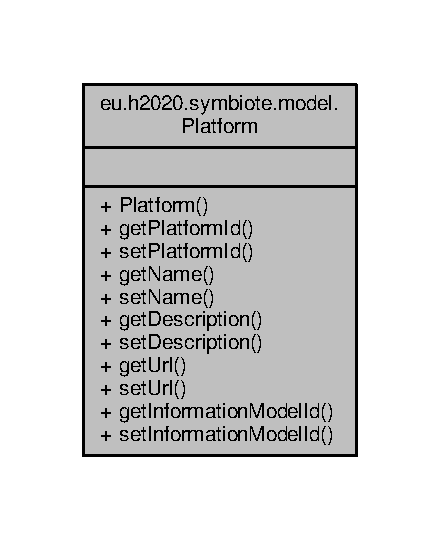
\includegraphics[width=211pt]{classeu_1_1h2020_1_1symbiote_1_1model_1_1Platform__coll__graph}
\end{center}
\end{figure}
\subsection*{Public Member Functions}
\begin{DoxyCompactItemize}
\item 
String {\bfseries get\+Platform\+Id} ()\hypertarget{classeu_1_1h2020_1_1symbiote_1_1model_1_1Platform_a2a09b94af05846adcf58f6405f0b1fdc}{}\label{classeu_1_1h2020_1_1symbiote_1_1model_1_1Platform_a2a09b94af05846adcf58f6405f0b1fdc}

\item 
void {\bfseries set\+Platform\+Id} (String platform\+Id)\hypertarget{classeu_1_1h2020_1_1symbiote_1_1model_1_1Platform_a3d9e886790d506f713e997f3c587e8ac}{}\label{classeu_1_1h2020_1_1symbiote_1_1model_1_1Platform_a3d9e886790d506f713e997f3c587e8ac}

\item 
String {\bfseries get\+Name} ()\hypertarget{classeu_1_1h2020_1_1symbiote_1_1model_1_1Platform_a9d39e85c470888c7043448f2eb059325}{}\label{classeu_1_1h2020_1_1symbiote_1_1model_1_1Platform_a9d39e85c470888c7043448f2eb059325}

\item 
void {\bfseries set\+Name} (String name)\hypertarget{classeu_1_1h2020_1_1symbiote_1_1model_1_1Platform_af4d5506c08659b3d71dcc8bf69c743ce}{}\label{classeu_1_1h2020_1_1symbiote_1_1model_1_1Platform_af4d5506c08659b3d71dcc8bf69c743ce}

\item 
String {\bfseries get\+Description} ()\hypertarget{classeu_1_1h2020_1_1symbiote_1_1model_1_1Platform_ad4a8d6cbb5ed57e241f783c512f052d9}{}\label{classeu_1_1h2020_1_1symbiote_1_1model_1_1Platform_ad4a8d6cbb5ed57e241f783c512f052d9}

\item 
void {\bfseries set\+Description} (String description)\hypertarget{classeu_1_1h2020_1_1symbiote_1_1model_1_1Platform_a9ec81f09b9fcd25ae264618591992cb2}{}\label{classeu_1_1h2020_1_1symbiote_1_1model_1_1Platform_a9ec81f09b9fcd25ae264618591992cb2}

\item 
String {\bfseries get\+Url} ()\hypertarget{classeu_1_1h2020_1_1symbiote_1_1model_1_1Platform_a4ca440b89e37c323dcb812ef07cfb66a}{}\label{classeu_1_1h2020_1_1symbiote_1_1model_1_1Platform_a4ca440b89e37c323dcb812ef07cfb66a}

\item 
void {\bfseries set\+Url} (String url)\hypertarget{classeu_1_1h2020_1_1symbiote_1_1model_1_1Platform_ac4d39a74475da2c2318cfd5e3667a5a1}{}\label{classeu_1_1h2020_1_1symbiote_1_1model_1_1Platform_ac4d39a74475da2c2318cfd5e3667a5a1}

\item 
String {\bfseries get\+Information\+Model\+Id} ()\hypertarget{classeu_1_1h2020_1_1symbiote_1_1model_1_1Platform_a799a5bb8e0665457c4b8bfd2b34c9b3c}{}\label{classeu_1_1h2020_1_1symbiote_1_1model_1_1Platform_a799a5bb8e0665457c4b8bfd2b34c9b3c}

\item 
void {\bfseries set\+Information\+Model\+Id} (String information\+Model\+Id)\hypertarget{classeu_1_1h2020_1_1symbiote_1_1model_1_1Platform_ae3e1cb93bcb289d575f215990d7e9499}{}\label{classeu_1_1h2020_1_1symbiote_1_1model_1_1Platform_ae3e1cb93bcb289d575f215990d7e9499}

\end{DoxyCompactItemize}


\subsection{Detailed Description}
Class representing platform in the system events. 

The documentation for this class was generated from the following file\+:\begin{DoxyCompactItemize}
\item 
src/main/java/eu/h2020/symbiote/model/Platform.\+java\end{DoxyCompactItemize}

\hypertarget{classeu_1_1h2020_1_1symbiote_1_1communication_1_1PlatformCreatedConsumer}{}\section{eu.\+h2020.\+symbiote.\+communication.\+Platform\+Created\+Consumer Class Reference}
\label{classeu_1_1h2020_1_1symbiote_1_1communication_1_1PlatformCreatedConsumer}\index{eu.\+h2020.\+symbiote.\+communication.\+Platform\+Created\+Consumer@{eu.\+h2020.\+symbiote.\+communication.\+Platform\+Created\+Consumer}}


Inheritance diagram for eu.\+h2020.\+symbiote.\+communication.\+Platform\+Created\+Consumer\+:
\nopagebreak
\begin{figure}[H]
\begin{center}
\leavevmode
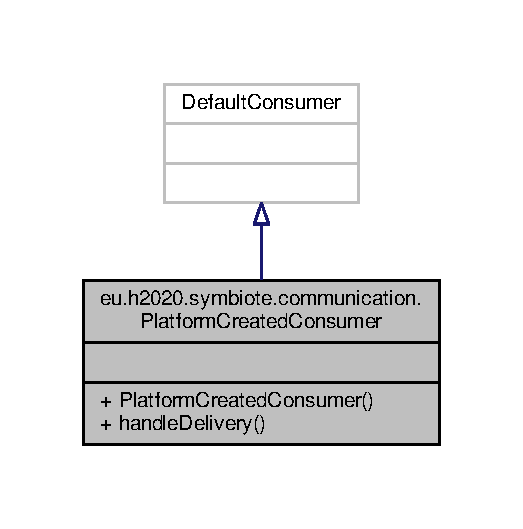
\includegraphics[width=251pt]{classeu_1_1h2020_1_1symbiote_1_1communication_1_1PlatformCreatedConsumer__inherit__graph}
\end{center}
\end{figure}


Collaboration diagram for eu.\+h2020.\+symbiote.\+communication.\+Platform\+Created\+Consumer\+:
\nopagebreak
\begin{figure}[H]
\begin{center}
\leavevmode
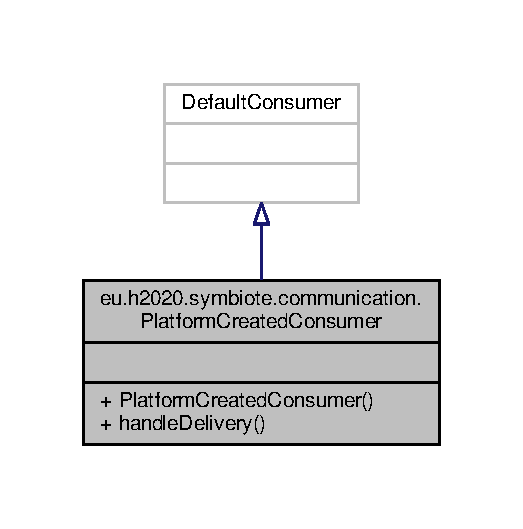
\includegraphics[width=251pt]{classeu_1_1h2020_1_1symbiote_1_1communication_1_1PlatformCreatedConsumer__coll__graph}
\end{center}
\end{figure}
\subsection*{Public Member Functions}
\begin{DoxyCompactItemize}
\item 
\hyperlink{classeu_1_1h2020_1_1symbiote_1_1communication_1_1PlatformCreatedConsumer_a2bf17b8b9e4f32394fb86c6724c05833}{Platform\+Created\+Consumer} (Channel channel, \hyperlink{classeu_1_1h2020_1_1symbiote_1_1handlers_1_1PlatformHandler}{Platform\+Handler} handler)
\item 
void {\bfseries handle\+Delivery} (String consumer\+Tag, Envelope envelope, A\+M\+Q\+P.\+Basic\+Properties properties, byte\mbox{[}$\,$\mbox{]} body)  throws I\+O\+Exception \hypertarget{classeu_1_1h2020_1_1symbiote_1_1communication_1_1PlatformCreatedConsumer_a357ddc796ad4d00c7545e4cf6252049d}{}\label{classeu_1_1h2020_1_1symbiote_1_1communication_1_1PlatformCreatedConsumer_a357ddc796ad4d00c7545e4cf6252049d}

\end{DoxyCompactItemize}


\subsection{Detailed Description}
Consumer of the platform created event. Handler creates R\+DF representation of provided platform and adds it into repository.

Created by Mael on 13/01/2017. 

\subsection{Constructor \& Destructor Documentation}
\index{eu\+::h2020\+::symbiote\+::communication\+::\+Platform\+Created\+Consumer@{eu\+::h2020\+::symbiote\+::communication\+::\+Platform\+Created\+Consumer}!Platform\+Created\+Consumer@{Platform\+Created\+Consumer}}
\index{Platform\+Created\+Consumer@{Platform\+Created\+Consumer}!eu\+::h2020\+::symbiote\+::communication\+::\+Platform\+Created\+Consumer@{eu\+::h2020\+::symbiote\+::communication\+::\+Platform\+Created\+Consumer}}
\subsubsection[{\texorpdfstring{Platform\+Created\+Consumer(\+Channel channel, Platform\+Handler handler)}{PlatformCreatedConsumer(Channel channel, PlatformHandler handler)}}]{\setlength{\rightskip}{0pt plus 5cm}eu.\+h2020.\+symbiote.\+communication.\+Platform\+Created\+Consumer.\+Platform\+Created\+Consumer (
\begin{DoxyParamCaption}
\item[{Channel}]{channel, }
\item[{{\bf Platform\+Handler}}]{handler}
\end{DoxyParamCaption}
)}\hypertarget{classeu_1_1h2020_1_1symbiote_1_1communication_1_1PlatformCreatedConsumer_a2bf17b8b9e4f32394fb86c6724c05833}{}\label{classeu_1_1h2020_1_1symbiote_1_1communication_1_1PlatformCreatedConsumer_a2bf17b8b9e4f32394fb86c6724c05833}
Constructs a new instance and records its association to the passed-\/in channel.


\begin{DoxyParams}{Parameters}
{\em channel} & the channel to which this consumer is attached. \\
\hline
{\em handler} & handler to be used by the consumer. \\
\hline
\end{DoxyParams}


The documentation for this class was generated from the following file\+:\begin{DoxyCompactItemize}
\item 
src/main/java/eu/h2020/symbiote/communication/Platform\+Created\+Consumer.\+java\end{DoxyCompactItemize}

\hypertarget{classeu_1_1h2020_1_1symbiote_1_1communication_1_1PlatformDeletedConsumer}{}\section{eu.\+h2020.\+symbiote.\+communication.\+Platform\+Deleted\+Consumer Class Reference}
\label{classeu_1_1h2020_1_1symbiote_1_1communication_1_1PlatformDeletedConsumer}\index{eu.\+h2020.\+symbiote.\+communication.\+Platform\+Deleted\+Consumer@{eu.\+h2020.\+symbiote.\+communication.\+Platform\+Deleted\+Consumer}}


Inheritance diagram for eu.\+h2020.\+symbiote.\+communication.\+Platform\+Deleted\+Consumer\+:
\nopagebreak
\begin{figure}[H]
\begin{center}
\leavevmode
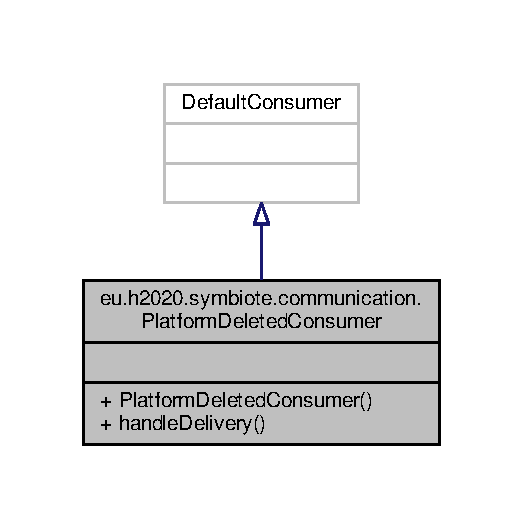
\includegraphics[width=251pt]{classeu_1_1h2020_1_1symbiote_1_1communication_1_1PlatformDeletedConsumer__inherit__graph}
\end{center}
\end{figure}


Collaboration diagram for eu.\+h2020.\+symbiote.\+communication.\+Platform\+Deleted\+Consumer\+:
\nopagebreak
\begin{figure}[H]
\begin{center}
\leavevmode
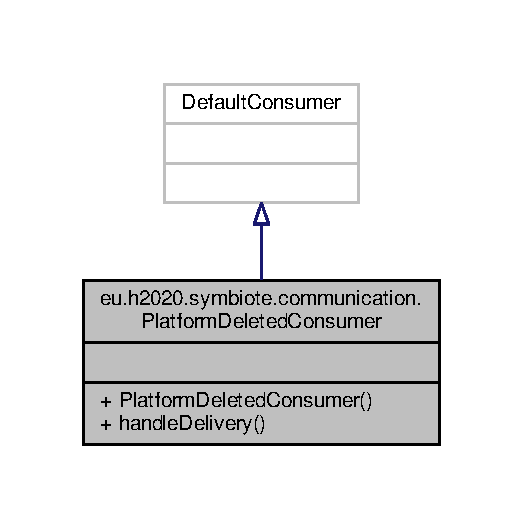
\includegraphics[width=251pt]{classeu_1_1h2020_1_1symbiote_1_1communication_1_1PlatformDeletedConsumer__coll__graph}
\end{center}
\end{figure}
\subsection*{Public Member Functions}
\begin{DoxyCompactItemize}
\item 
\hyperlink{classeu_1_1h2020_1_1symbiote_1_1communication_1_1PlatformDeletedConsumer_aa5c0d07fd609f512d0e504edd05e7c11}{Platform\+Deleted\+Consumer} (Channel channel, \hyperlink{classeu_1_1h2020_1_1symbiote_1_1handlers_1_1PlatformHandler}{Platform\+Handler} handler)
\item 
void {\bfseries handle\+Delivery} (String consumer\+Tag, Envelope envelope, A\+M\+Q\+P.\+Basic\+Properties properties, byte\mbox{[}$\,$\mbox{]} body)  throws I\+O\+Exception \hypertarget{classeu_1_1h2020_1_1symbiote_1_1communication_1_1PlatformDeletedConsumer_a5ef55cd2aac005349910ef91b0f27e5e}{}\label{classeu_1_1h2020_1_1symbiote_1_1communication_1_1PlatformDeletedConsumer_a5ef55cd2aac005349910ef91b0f27e5e}

\end{DoxyCompactItemize}


\subsection{Detailed Description}
Consumer of the platform deleted event. Handler removes R\+DF representation of specified platform.

Created by Mael on 13/01/2017. 

\subsection{Constructor \& Destructor Documentation}
\index{eu\+::h2020\+::symbiote\+::communication\+::\+Platform\+Deleted\+Consumer@{eu\+::h2020\+::symbiote\+::communication\+::\+Platform\+Deleted\+Consumer}!Platform\+Deleted\+Consumer@{Platform\+Deleted\+Consumer}}
\index{Platform\+Deleted\+Consumer@{Platform\+Deleted\+Consumer}!eu\+::h2020\+::symbiote\+::communication\+::\+Platform\+Deleted\+Consumer@{eu\+::h2020\+::symbiote\+::communication\+::\+Platform\+Deleted\+Consumer}}
\subsubsection[{\texorpdfstring{Platform\+Deleted\+Consumer(\+Channel channel, Platform\+Handler handler)}{PlatformDeletedConsumer(Channel channel, PlatformHandler handler)}}]{\setlength{\rightskip}{0pt plus 5cm}eu.\+h2020.\+symbiote.\+communication.\+Platform\+Deleted\+Consumer.\+Platform\+Deleted\+Consumer (
\begin{DoxyParamCaption}
\item[{Channel}]{channel, }
\item[{{\bf Platform\+Handler}}]{handler}
\end{DoxyParamCaption}
)}\hypertarget{classeu_1_1h2020_1_1symbiote_1_1communication_1_1PlatformDeletedConsumer_aa5c0d07fd609f512d0e504edd05e7c11}{}\label{classeu_1_1h2020_1_1symbiote_1_1communication_1_1PlatformDeletedConsumer_aa5c0d07fd609f512d0e504edd05e7c11}
Constructs a new instance and records its association to the passed-\/in channel.


\begin{DoxyParams}{Parameters}
{\em channel} & the channel to which this consumer is attached. \\
\hline
{\em handler} & handler to be used by the consumer. \\
\hline
\end{DoxyParams}


The documentation for this class was generated from the following file\+:\begin{DoxyCompactItemize}
\item 
src/main/java/eu/h2020/symbiote/communication/Platform\+Deleted\+Consumer.\+java\end{DoxyCompactItemize}

\hypertarget{classeu_1_1h2020_1_1symbiote_1_1handlers_1_1PlatformHandler}{}\section{eu.\+h2020.\+symbiote.\+handlers.\+Platform\+Handler Class Reference}
\label{classeu_1_1h2020_1_1symbiote_1_1handlers_1_1PlatformHandler}\index{eu.\+h2020.\+symbiote.\+handlers.\+Platform\+Handler@{eu.\+h2020.\+symbiote.\+handlers.\+Platform\+Handler}}


Inheritance diagram for eu.\+h2020.\+symbiote.\+handlers.\+Platform\+Handler\+:
\nopagebreak
\begin{figure}[H]
\begin{center}
\leavevmode
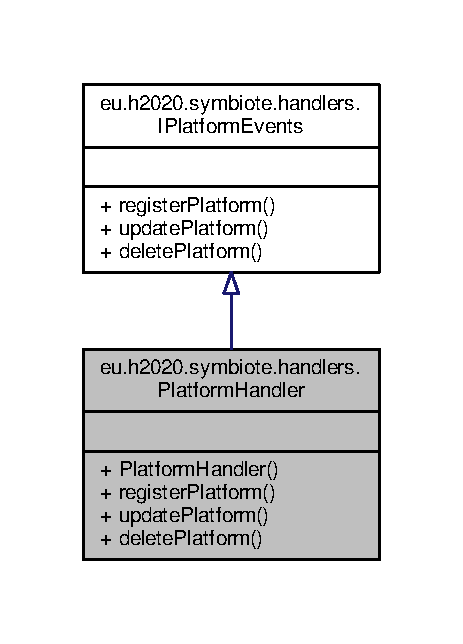
\includegraphics[width=222pt]{classeu_1_1h2020_1_1symbiote_1_1handlers_1_1PlatformHandler__inherit__graph}
\end{center}
\end{figure}


Collaboration diagram for eu.\+h2020.\+symbiote.\+handlers.\+Platform\+Handler\+:
\nopagebreak
\begin{figure}[H]
\begin{center}
\leavevmode
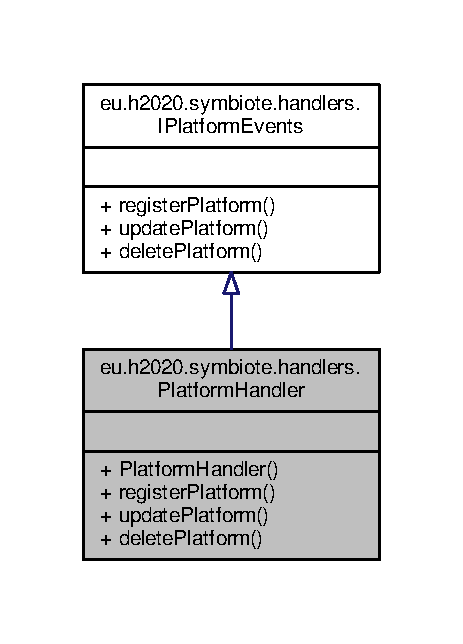
\includegraphics[width=222pt]{classeu_1_1h2020_1_1symbiote_1_1handlers_1_1PlatformHandler__coll__graph}
\end{center}
\end{figure}
\subsection*{Public Member Functions}
\begin{DoxyCompactItemize}
\item 
\hyperlink{classeu_1_1h2020_1_1symbiote_1_1handlers_1_1PlatformHandler_ad9131f7d4698a8a04f2a96627564c224}{Platform\+Handler} (\hyperlink{classeu_1_1h2020_1_1symbiote_1_1search_1_1SearchStorage}{Search\+Storage} storage)
\item 
boolean \hyperlink{classeu_1_1h2020_1_1symbiote_1_1handlers_1_1PlatformHandler_a88a6b019f2d95821ee3f17c8f6c572a9}{register\+Platform} (\hyperlink{classeu_1_1h2020_1_1symbiote_1_1model_1_1Platform}{Platform} platform)
\item 
boolean \hyperlink{classeu_1_1h2020_1_1symbiote_1_1handlers_1_1PlatformHandler_ac4701e47973cb2061607dc9ee2916393}{update\+Platform} (\hyperlink{classeu_1_1h2020_1_1symbiote_1_1model_1_1Platform}{Platform} platform)
\item 
boolean \hyperlink{classeu_1_1h2020_1_1symbiote_1_1handlers_1_1PlatformHandler_a3c20ba0a131ad392eb74dd481548a062}{delete\+Platform} (String platform\+Id)
\end{DoxyCompactItemize}


\subsection{Detailed Description}
Implementation of the handler for the platform related events.

Created by Mael on 11/01/2017. 

\subsection{Constructor \& Destructor Documentation}
\index{eu\+::h2020\+::symbiote\+::handlers\+::\+Platform\+Handler@{eu\+::h2020\+::symbiote\+::handlers\+::\+Platform\+Handler}!Platform\+Handler@{Platform\+Handler}}
\index{Platform\+Handler@{Platform\+Handler}!eu\+::h2020\+::symbiote\+::handlers\+::\+Platform\+Handler@{eu\+::h2020\+::symbiote\+::handlers\+::\+Platform\+Handler}}
\subsubsection[{\texorpdfstring{Platform\+Handler(\+Search\+Storage storage)}{PlatformHandler(SearchStorage storage)}}]{\setlength{\rightskip}{0pt plus 5cm}eu.\+h2020.\+symbiote.\+handlers.\+Platform\+Handler.\+Platform\+Handler (
\begin{DoxyParamCaption}
\item[{{\bf Search\+Storage}}]{storage}
\end{DoxyParamCaption}
)}\hypertarget{classeu_1_1h2020_1_1symbiote_1_1handlers_1_1PlatformHandler_ad9131f7d4698a8a04f2a96627564c224}{}\label{classeu_1_1h2020_1_1symbiote_1_1handlers_1_1PlatformHandler_ad9131f7d4698a8a04f2a96627564c224}
Create a handler of the platform events for specified storage.


\begin{DoxyParams}{Parameters}
{\em storage} & Storage on which the events should be executed. \\
\hline
\end{DoxyParams}


\subsection{Member Function Documentation}
\index{eu\+::h2020\+::symbiote\+::handlers\+::\+Platform\+Handler@{eu\+::h2020\+::symbiote\+::handlers\+::\+Platform\+Handler}!delete\+Platform@{delete\+Platform}}
\index{delete\+Platform@{delete\+Platform}!eu\+::h2020\+::symbiote\+::handlers\+::\+Platform\+Handler@{eu\+::h2020\+::symbiote\+::handlers\+::\+Platform\+Handler}}
\subsubsection[{\texorpdfstring{delete\+Platform(\+String platform\+Id)}{deletePlatform(String platformId)}}]{\setlength{\rightskip}{0pt plus 5cm}boolean eu.\+h2020.\+symbiote.\+handlers.\+Platform\+Handler.\+delete\+Platform (
\begin{DoxyParamCaption}
\item[{String}]{platform\+Id}
\end{DoxyParamCaption}
)}\hypertarget{classeu_1_1h2020_1_1symbiote_1_1handlers_1_1PlatformHandler_a3c20ba0a131ad392eb74dd481548a062}{}\label{classeu_1_1h2020_1_1symbiote_1_1handlers_1_1PlatformHandler_a3c20ba0a131ad392eb74dd481548a062}
Deletes platform representation in the Apache Jena repository.


\begin{DoxyParams}{Parameters}
{\em platform\+Id} & Id of the platform to be deleted \\
\hline
\end{DoxyParams}
\begin{DoxyReturn}{Returns}
{\ttfamily true} if delete was successful. 
\end{DoxyReturn}


Implements \hyperlink{interfaceeu_1_1h2020_1_1symbiote_1_1handlers_1_1IPlatformEvents_aaa59c8d1b1d80f4e58e20227a78c1f23}{eu.\+h2020.\+symbiote.\+handlers.\+I\+Platform\+Events}.

\index{eu\+::h2020\+::symbiote\+::handlers\+::\+Platform\+Handler@{eu\+::h2020\+::symbiote\+::handlers\+::\+Platform\+Handler}!register\+Platform@{register\+Platform}}
\index{register\+Platform@{register\+Platform}!eu\+::h2020\+::symbiote\+::handlers\+::\+Platform\+Handler@{eu\+::h2020\+::symbiote\+::handlers\+::\+Platform\+Handler}}
\subsubsection[{\texorpdfstring{register\+Platform(\+Platform platform)}{registerPlatform(Platform platform)}}]{\setlength{\rightskip}{0pt plus 5cm}boolean eu.\+h2020.\+symbiote.\+handlers.\+Platform\+Handler.\+register\+Platform (
\begin{DoxyParamCaption}
\item[{{\bf Platform}}]{platform}
\end{DoxyParamCaption}
)}\hypertarget{classeu_1_1h2020_1_1symbiote_1_1handlers_1_1PlatformHandler_a88a6b019f2d95821ee3f17c8f6c572a9}{}\label{classeu_1_1h2020_1_1symbiote_1_1handlers_1_1PlatformHandler_a88a6b019f2d95821ee3f17c8f6c572a9}
Registers platform representation in the Apache Jena repository.


\begin{DoxyParams}{Parameters}
{\em platform} & Platform to be saved \\
\hline
\end{DoxyParams}
\begin{DoxyReturn}{Returns}
{\ttfamily true} if registration was successful. 
\end{DoxyReturn}


Implements \hyperlink{interfaceeu_1_1h2020_1_1symbiote_1_1handlers_1_1IPlatformEvents_a02c6e32eb7af9a13b584a5c911ab8d8c}{eu.\+h2020.\+symbiote.\+handlers.\+I\+Platform\+Events}.

\index{eu\+::h2020\+::symbiote\+::handlers\+::\+Platform\+Handler@{eu\+::h2020\+::symbiote\+::handlers\+::\+Platform\+Handler}!update\+Platform@{update\+Platform}}
\index{update\+Platform@{update\+Platform}!eu\+::h2020\+::symbiote\+::handlers\+::\+Platform\+Handler@{eu\+::h2020\+::symbiote\+::handlers\+::\+Platform\+Handler}}
\subsubsection[{\texorpdfstring{update\+Platform(\+Platform platform)}{updatePlatform(Platform platform)}}]{\setlength{\rightskip}{0pt plus 5cm}boolean eu.\+h2020.\+symbiote.\+handlers.\+Platform\+Handler.\+update\+Platform (
\begin{DoxyParamCaption}
\item[{{\bf Platform}}]{platform}
\end{DoxyParamCaption}
)}\hypertarget{classeu_1_1h2020_1_1symbiote_1_1handlers_1_1PlatformHandler_ac4701e47973cb2061607dc9ee2916393}{}\label{classeu_1_1h2020_1_1symbiote_1_1handlers_1_1PlatformHandler_ac4701e47973cb2061607dc9ee2916393}
Updates platform representation in the Apache Jena repository.


\begin{DoxyParams}{Parameters}
{\em platform} & Platform to be updated \\
\hline
\end{DoxyParams}
\begin{DoxyReturn}{Returns}
{\ttfamily true} if update was successful. 
\end{DoxyReturn}


Implements \hyperlink{interfaceeu_1_1h2020_1_1symbiote_1_1handlers_1_1IPlatformEvents_ad5b491b150e4015525e9985143bbfcd3}{eu.\+h2020.\+symbiote.\+handlers.\+I\+Platform\+Events}.



The documentation for this class was generated from the following file\+:\begin{DoxyCompactItemize}
\item 
src/main/java/eu/h2020/symbiote/handlers/Platform\+Handler.\+java\end{DoxyCompactItemize}

\hypertarget{classeu_1_1h2020_1_1symbiote_1_1communication_1_1PlatformModifiedConsumer}{}\section{eu.\+h2020.\+symbiote.\+communication.\+Platform\+Modified\+Consumer Class Reference}
\label{classeu_1_1h2020_1_1symbiote_1_1communication_1_1PlatformModifiedConsumer}\index{eu.\+h2020.\+symbiote.\+communication.\+Platform\+Modified\+Consumer@{eu.\+h2020.\+symbiote.\+communication.\+Platform\+Modified\+Consumer}}


Inheritance diagram for eu.\+h2020.\+symbiote.\+communication.\+Platform\+Modified\+Consumer\+:
\nopagebreak
\begin{figure}[H]
\begin{center}
\leavevmode
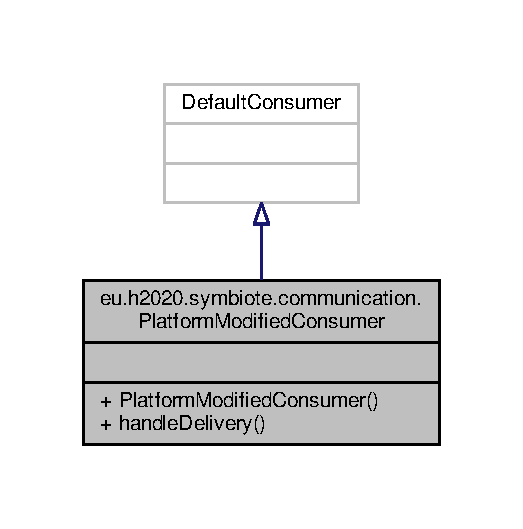
\includegraphics[width=251pt]{classeu_1_1h2020_1_1symbiote_1_1communication_1_1PlatformModifiedConsumer__inherit__graph}
\end{center}
\end{figure}


Collaboration diagram for eu.\+h2020.\+symbiote.\+communication.\+Platform\+Modified\+Consumer\+:
\nopagebreak
\begin{figure}[H]
\begin{center}
\leavevmode
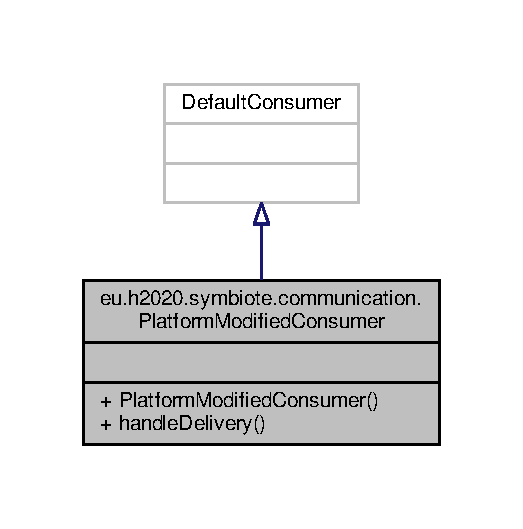
\includegraphics[width=251pt]{classeu_1_1h2020_1_1symbiote_1_1communication_1_1PlatformModifiedConsumer__coll__graph}
\end{center}
\end{figure}
\subsection*{Public Member Functions}
\begin{DoxyCompactItemize}
\item 
\hyperlink{classeu_1_1h2020_1_1symbiote_1_1communication_1_1PlatformModifiedConsumer_ad9b04b6ba41b1d6280f63f1a458e3348}{Platform\+Modified\+Consumer} (Channel channel, \hyperlink{classeu_1_1h2020_1_1symbiote_1_1handlers_1_1PlatformHandler}{Platform\+Handler} handler)
\item 
void {\bfseries handle\+Delivery} (String consumer\+Tag, Envelope envelope, A\+M\+Q\+P.\+Basic\+Properties properties, byte\mbox{[}$\,$\mbox{]} body)  throws I\+O\+Exception \hypertarget{classeu_1_1h2020_1_1symbiote_1_1communication_1_1PlatformModifiedConsumer_a8e821b65d946c3c63c349507eab2c285}{}\label{classeu_1_1h2020_1_1symbiote_1_1communication_1_1PlatformModifiedConsumer_a8e821b65d946c3c63c349507eab2c285}

\end{DoxyCompactItemize}


\subsection{Detailed Description}
Consumer of the platform modified event. Handler creates S\+P\+A\+R\+QL Update Delete/\+Insert representation of modifed platform and executes it.

Created by Mael on 13/01/2017. 

\subsection{Constructor \& Destructor Documentation}
\index{eu\+::h2020\+::symbiote\+::communication\+::\+Platform\+Modified\+Consumer@{eu\+::h2020\+::symbiote\+::communication\+::\+Platform\+Modified\+Consumer}!Platform\+Modified\+Consumer@{Platform\+Modified\+Consumer}}
\index{Platform\+Modified\+Consumer@{Platform\+Modified\+Consumer}!eu\+::h2020\+::symbiote\+::communication\+::\+Platform\+Modified\+Consumer@{eu\+::h2020\+::symbiote\+::communication\+::\+Platform\+Modified\+Consumer}}
\subsubsection[{\texorpdfstring{Platform\+Modified\+Consumer(\+Channel channel, Platform\+Handler handler)}{PlatformModifiedConsumer(Channel channel, PlatformHandler handler)}}]{\setlength{\rightskip}{0pt plus 5cm}eu.\+h2020.\+symbiote.\+communication.\+Platform\+Modified\+Consumer.\+Platform\+Modified\+Consumer (
\begin{DoxyParamCaption}
\item[{Channel}]{channel, }
\item[{{\bf Platform\+Handler}}]{handler}
\end{DoxyParamCaption}
)}\hypertarget{classeu_1_1h2020_1_1symbiote_1_1communication_1_1PlatformModifiedConsumer_ad9b04b6ba41b1d6280f63f1a458e3348}{}\label{classeu_1_1h2020_1_1symbiote_1_1communication_1_1PlatformModifiedConsumer_ad9b04b6ba41b1d6280f63f1a458e3348}
Constructs a new instance and records its association to the passed-\/in channel.


\begin{DoxyParams}{Parameters}
{\em channel} & the channel to which this consumer is attached. \\
\hline
{\em handler} & handler to be used by the consumer. \\
\hline
\end{DoxyParams}


The documentation for this class was generated from the following file\+:\begin{DoxyCompactItemize}
\item 
src/main/java/eu/h2020/symbiote/communication/Platform\+Modified\+Consumer.\+java\end{DoxyCompactItemize}

\hypertarget{classeu_1_1h2020_1_1symbiote_1_1query_1_1QueryGenerator}{}\section{eu.\+h2020.\+symbiote.\+query.\+Query\+Generator Class Reference}
\label{classeu_1_1h2020_1_1symbiote_1_1query_1_1QueryGenerator}\index{eu.\+h2020.\+symbiote.\+query.\+Query\+Generator@{eu.\+h2020.\+symbiote.\+query.\+Query\+Generator}}


Collaboration diagram for eu.\+h2020.\+symbiote.\+query.\+Query\+Generator\+:
\nopagebreak
\begin{figure}[H]
\begin{center}
\leavevmode
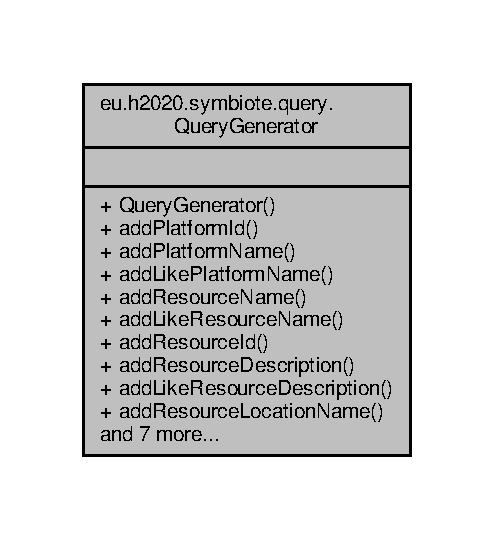
\includegraphics[width=237pt]{classeu_1_1h2020_1_1symbiote_1_1query_1_1QueryGenerator__coll__graph}
\end{center}
\end{figure}
\subsection*{Public Member Functions}
\begin{DoxyCompactItemize}
\item 
\hyperlink{classeu_1_1h2020_1_1symbiote_1_1query_1_1QueryGenerator}{Query\+Generator} {\bfseries add\+Platform\+Id} (String platform\+Id)\hypertarget{classeu_1_1h2020_1_1symbiote_1_1query_1_1QueryGenerator_a343acf8af004a11d7e8e9e6ce8f43855}{}\label{classeu_1_1h2020_1_1symbiote_1_1query_1_1QueryGenerator_a343acf8af004a11d7e8e9e6ce8f43855}

\item 
\hyperlink{classeu_1_1h2020_1_1symbiote_1_1query_1_1QueryGenerator}{Query\+Generator} {\bfseries add\+Platform\+Name} (String platform\+Name)\hypertarget{classeu_1_1h2020_1_1symbiote_1_1query_1_1QueryGenerator_a363f3573bce42e9c9173bb299ba6692b}{}\label{classeu_1_1h2020_1_1symbiote_1_1query_1_1QueryGenerator_a363f3573bce42e9c9173bb299ba6692b}

\item 
\hyperlink{classeu_1_1h2020_1_1symbiote_1_1query_1_1QueryGenerator}{Query\+Generator} {\bfseries add\+Like\+Platform\+Name} (String platform\+Name, String command)\hypertarget{classeu_1_1h2020_1_1symbiote_1_1query_1_1QueryGenerator_a252964b69c003dd49d94fe804f0101d0}{}\label{classeu_1_1h2020_1_1symbiote_1_1query_1_1QueryGenerator_a252964b69c003dd49d94fe804f0101d0}

\item 
\hyperlink{classeu_1_1h2020_1_1symbiote_1_1query_1_1QueryGenerator}{Query\+Generator} {\bfseries add\+Resource\+Name} (String resource\+Name)\hypertarget{classeu_1_1h2020_1_1symbiote_1_1query_1_1QueryGenerator_a5106c210fb367ee7de138087f35cf59a}{}\label{classeu_1_1h2020_1_1symbiote_1_1query_1_1QueryGenerator_a5106c210fb367ee7de138087f35cf59a}

\item 
\hyperlink{classeu_1_1h2020_1_1symbiote_1_1query_1_1QueryGenerator}{Query\+Generator} {\bfseries add\+Like\+Resource\+Name} (String resource\+Name, String command)\hypertarget{classeu_1_1h2020_1_1symbiote_1_1query_1_1QueryGenerator_a43eef490f07d9bf683715eba6e9ca33e}{}\label{classeu_1_1h2020_1_1symbiote_1_1query_1_1QueryGenerator_a43eef490f07d9bf683715eba6e9ca33e}

\item 
\hyperlink{classeu_1_1h2020_1_1symbiote_1_1query_1_1QueryGenerator}{Query\+Generator} {\bfseries add\+Resource\+Id} (String resource\+Id)\hypertarget{classeu_1_1h2020_1_1symbiote_1_1query_1_1QueryGenerator_a1734b1888a91c327976feaeaa1c1f0ba}{}\label{classeu_1_1h2020_1_1symbiote_1_1query_1_1QueryGenerator_a1734b1888a91c327976feaeaa1c1f0ba}

\item 
\hyperlink{classeu_1_1h2020_1_1symbiote_1_1query_1_1QueryGenerator}{Query\+Generator} {\bfseries add\+Resource\+Description} (String resource\+Description)\hypertarget{classeu_1_1h2020_1_1symbiote_1_1query_1_1QueryGenerator_a811289fd4a4ca55e407c56ba94da42a9}{}\label{classeu_1_1h2020_1_1symbiote_1_1query_1_1QueryGenerator_a811289fd4a4ca55e407c56ba94da42a9}

\item 
\hyperlink{classeu_1_1h2020_1_1symbiote_1_1query_1_1QueryGenerator}{Query\+Generator} {\bfseries add\+Like\+Resource\+Description} (String resource\+Description, String command)\hypertarget{classeu_1_1h2020_1_1symbiote_1_1query_1_1QueryGenerator_afa8ef3cc65ffbfdf2fd1dc948634ed52}{}\label{classeu_1_1h2020_1_1symbiote_1_1query_1_1QueryGenerator_afa8ef3cc65ffbfdf2fd1dc948634ed52}

\item 
\hyperlink{classeu_1_1h2020_1_1symbiote_1_1query_1_1QueryGenerator}{Query\+Generator} {\bfseries add\+Resource\+Location\+Name} (String location\+Name)\hypertarget{classeu_1_1h2020_1_1symbiote_1_1query_1_1QueryGenerator_a1a2e936bbedefbca381953afd0467e4e}{}\label{classeu_1_1h2020_1_1symbiote_1_1query_1_1QueryGenerator_a1a2e936bbedefbca381953afd0467e4e}

\item 
\hyperlink{classeu_1_1h2020_1_1symbiote_1_1query_1_1QueryGenerator}{Query\+Generator} {\bfseries add\+Like\+Resource\+Location\+Name} (String location\+Name, String command)\hypertarget{classeu_1_1h2020_1_1symbiote_1_1query_1_1QueryGenerator_a0b182a5fe22d5c409a26d99a3be90eba}{}\label{classeu_1_1h2020_1_1symbiote_1_1query_1_1QueryGenerator_a0b182a5fe22d5c409a26d99a3be90eba}

\item 
\hyperlink{classeu_1_1h2020_1_1symbiote_1_1query_1_1QueryGenerator}{Query\+Generator} {\bfseries add\+Resource\+Location\+Distance} (Double latitude, Double longitude, Integer distance)\hypertarget{classeu_1_1h2020_1_1symbiote_1_1query_1_1QueryGenerator_a49f34146c17f6e550acdebf86930b3ec}{}\label{classeu_1_1h2020_1_1symbiote_1_1query_1_1QueryGenerator_a49f34146c17f6e550acdebf86930b3ec}

\item 
\hyperlink{classeu_1_1h2020_1_1symbiote_1_1query_1_1QueryGenerator}{Query\+Generator} {\bfseries add\+Resource\+Observed\+Property\+Name} (String property\+Name)\hypertarget{classeu_1_1h2020_1_1symbiote_1_1query_1_1QueryGenerator_ad7c012c8f3eafc59dcfa8fe56e5aff34}{}\label{classeu_1_1h2020_1_1symbiote_1_1query_1_1QueryGenerator_ad7c012c8f3eafc59dcfa8fe56e5aff34}

\item 
\hyperlink{classeu_1_1h2020_1_1symbiote_1_1query_1_1QueryGenerator}{Query\+Generator} {\bfseries add\+Like\+Resource\+Observed\+Property\+Name} (String property\+Name, String command)\hypertarget{classeu_1_1h2020_1_1symbiote_1_1query_1_1QueryGenerator_a69e76d3e08335d404ec0af8626c58e2c}{}\label{classeu_1_1h2020_1_1symbiote_1_1query_1_1QueryGenerator_a69e76d3e08335d404ec0af8626c58e2c}

\item 
\hyperlink{classeu_1_1h2020_1_1symbiote_1_1query_1_1QueryGenerator}{Query\+Generator} {\bfseries add\+Resource\+Observed\+Property\+Names} (List$<$ String $>$ property\+Names)\hypertarget{classeu_1_1h2020_1_1symbiote_1_1query_1_1QueryGenerator_a925f75c04a7e608619882dc683d60b1c}{}\label{classeu_1_1h2020_1_1symbiote_1_1query_1_1QueryGenerator_a925f75c04a7e608619882dc683d60b1c}

\item 
String {\bfseries to\+String} ()\hypertarget{classeu_1_1h2020_1_1symbiote_1_1query_1_1QueryGenerator_a1b90b36cb12b3e63d485eccac837d6d0}{}\label{classeu_1_1h2020_1_1symbiote_1_1query_1_1QueryGenerator_a1b90b36cb12b3e63d485eccac837d6d0}

\item 
boolean {\bfseries is\+Multivaluequery} ()\hypertarget{classeu_1_1h2020_1_1symbiote_1_1query_1_1QueryGenerator_a330e5262e01af4a187fc754529285f0d}{}\label{classeu_1_1h2020_1_1symbiote_1_1query_1_1QueryGenerator_a330e5262e01af4a187fc754529285f0d}

\end{DoxyCompactItemize}


\subsection{Detailed Description}
Class used to generate S\+P\+A\+R\+QL query reflecting specified parameters of the query to the Search

Created by Mael on 23/01/2017. 

The documentation for this class was generated from the following file\+:\begin{DoxyCompactItemize}
\item 
src/main/java/eu/h2020/symbiote/query/Query\+Generator.\+java\end{DoxyCompactItemize}

\hypertarget{classeu_1_1h2020_1_1symbiote_1_1model_1_1QueryRequest}{}\section{eu.\+h2020.\+symbiote.\+model.\+Query\+Request Class Reference}
\label{classeu_1_1h2020_1_1symbiote_1_1model_1_1QueryRequest}\index{eu.\+h2020.\+symbiote.\+model.\+Query\+Request@{eu.\+h2020.\+symbiote.\+model.\+Query\+Request}}


Collaboration diagram for eu.\+h2020.\+symbiote.\+model.\+Query\+Request\+:
\nopagebreak
\begin{figure}[H]
\begin{center}
\leavevmode
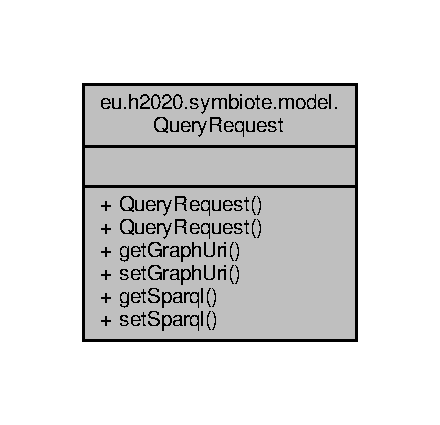
\includegraphics[width=211pt]{classeu_1_1h2020_1_1symbiote_1_1model_1_1QueryRequest__coll__graph}
\end{center}
\end{figure}
\subsection*{Public Member Functions}
\begin{DoxyCompactItemize}
\item 
{\bfseries Query\+Request} (String sparql, String graph\+Uri)\hypertarget{classeu_1_1h2020_1_1symbiote_1_1model_1_1QueryRequest_aceafa1a43808d053112665e422b10e8a}{}\label{classeu_1_1h2020_1_1symbiote_1_1model_1_1QueryRequest_aceafa1a43808d053112665e422b10e8a}

\item 
String {\bfseries get\+Graph\+Uri} ()\hypertarget{classeu_1_1h2020_1_1symbiote_1_1model_1_1QueryRequest_aebc84bcc3c9706d6f8856a02f974834c}{}\label{classeu_1_1h2020_1_1symbiote_1_1model_1_1QueryRequest_aebc84bcc3c9706d6f8856a02f974834c}

\item 
void {\bfseries set\+Graph\+Uri} (String graph\+Uri)\hypertarget{classeu_1_1h2020_1_1symbiote_1_1model_1_1QueryRequest_add4593940902dfbd1342ab57a771a353}{}\label{classeu_1_1h2020_1_1symbiote_1_1model_1_1QueryRequest_add4593940902dfbd1342ab57a771a353}

\item 
String {\bfseries get\+Sparql} ()\hypertarget{classeu_1_1h2020_1_1symbiote_1_1model_1_1QueryRequest_a4b337bbff009caa70dcd668035fa1f91}{}\label{classeu_1_1h2020_1_1symbiote_1_1model_1_1QueryRequest_a4b337bbff009caa70dcd668035fa1f91}

\item 
void {\bfseries set\+Sparql} (String sparql)\hypertarget{classeu_1_1h2020_1_1symbiote_1_1model_1_1QueryRequest_a7548ea81d796ca6ed03af66a7bd059fe}{}\label{classeu_1_1h2020_1_1symbiote_1_1model_1_1QueryRequest_a7548ea81d796ca6ed03af66a7bd059fe}

\end{DoxyCompactItemize}


\subsection{Detailed Description}
Created by Mael on 23/01/2017. 

The documentation for this class was generated from the following file\+:\begin{DoxyCompactItemize}
\item 
src/main/java/eu/h2020/symbiote/model/Query\+Request.\+java\end{DoxyCompactItemize}

\hypertarget{interfaceeu_1_1h2020_1_1symbiote_1_1query_1_1QueryVarName}{}\section{eu.\+h2020.\+symbiote.\+query.\+Query\+Var\+Name Interface Reference}
\label{interfaceeu_1_1h2020_1_1symbiote_1_1query_1_1QueryVarName}\index{eu.\+h2020.\+symbiote.\+query.\+Query\+Var\+Name@{eu.\+h2020.\+symbiote.\+query.\+Query\+Var\+Name}}


Collaboration diagram for eu.\+h2020.\+symbiote.\+query.\+Query\+Var\+Name\+:
\nopagebreak
\begin{figure}[H]
\begin{center}
\leavevmode
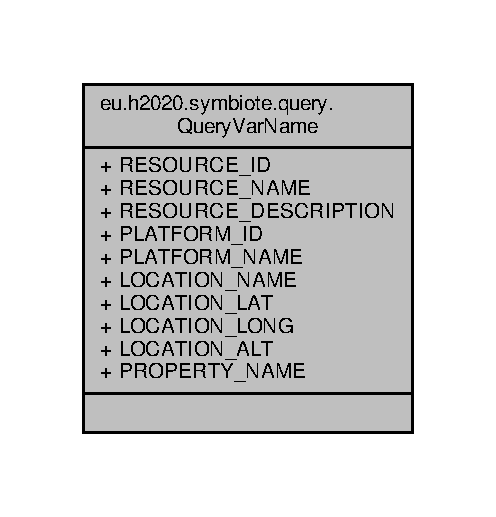
\includegraphics[width=238pt]{interfaceeu_1_1h2020_1_1symbiote_1_1query_1_1QueryVarName__coll__graph}
\end{center}
\end{figure}
\subsection*{Public Attributes}
\begin{DoxyCompactItemize}
\item 
String {\bfseries R\+E\+S\+O\+U\+R\+C\+E\+\_\+\+ID} = \char`\"{}res\+Id\char`\"{}\hypertarget{interfaceeu_1_1h2020_1_1symbiote_1_1query_1_1QueryVarName_ac3c0ea6b252a936f52b6ee931a8a17a1}{}\label{interfaceeu_1_1h2020_1_1symbiote_1_1query_1_1QueryVarName_ac3c0ea6b252a936f52b6ee931a8a17a1}

\item 
String {\bfseries R\+E\+S\+O\+U\+R\+C\+E\+\_\+\+N\+A\+ME} = \char`\"{}res\+Name\char`\"{}\hypertarget{interfaceeu_1_1h2020_1_1symbiote_1_1query_1_1QueryVarName_a66418233765e3fc1ffa71a1d79bf5f62}{}\label{interfaceeu_1_1h2020_1_1symbiote_1_1query_1_1QueryVarName_a66418233765e3fc1ffa71a1d79bf5f62}

\item 
String {\bfseries R\+E\+S\+O\+U\+R\+C\+E\+\_\+\+D\+E\+S\+C\+R\+I\+P\+T\+I\+ON} = \char`\"{}res\+Description\char`\"{}\hypertarget{interfaceeu_1_1h2020_1_1symbiote_1_1query_1_1QueryVarName_ac9f5abb59a5bb271fc673449980b19ea}{}\label{interfaceeu_1_1h2020_1_1symbiote_1_1query_1_1QueryVarName_ac9f5abb59a5bb271fc673449980b19ea}

\item 
String {\bfseries P\+L\+A\+T\+F\+O\+R\+M\+\_\+\+ID} = \char`\"{}platform\+Id\char`\"{}\hypertarget{interfaceeu_1_1h2020_1_1symbiote_1_1query_1_1QueryVarName_a204fad74df4daf04f04321e6d7b0dcad}{}\label{interfaceeu_1_1h2020_1_1symbiote_1_1query_1_1QueryVarName_a204fad74df4daf04f04321e6d7b0dcad}

\item 
String {\bfseries P\+L\+A\+T\+F\+O\+R\+M\+\_\+\+N\+A\+ME} = \char`\"{}platform\+Name\char`\"{}\hypertarget{interfaceeu_1_1h2020_1_1symbiote_1_1query_1_1QueryVarName_a237b6e8b9c43ff627bb1488ae587cd9b}{}\label{interfaceeu_1_1h2020_1_1symbiote_1_1query_1_1QueryVarName_a237b6e8b9c43ff627bb1488ae587cd9b}

\item 
String {\bfseries L\+O\+C\+A\+T\+I\+O\+N\+\_\+\+N\+A\+ME} = \char`\"{}location\+Name\char`\"{}\hypertarget{interfaceeu_1_1h2020_1_1symbiote_1_1query_1_1QueryVarName_ad32768d3f518b81dd7d78315453a5444}{}\label{interfaceeu_1_1h2020_1_1symbiote_1_1query_1_1QueryVarName_ad32768d3f518b81dd7d78315453a5444}

\item 
String {\bfseries L\+O\+C\+A\+T\+I\+O\+N\+\_\+\+L\+AT} = \char`\"{}location\+Lat\char`\"{}\hypertarget{interfaceeu_1_1h2020_1_1symbiote_1_1query_1_1QueryVarName_ac9b9dc6e731be6f40ca4d3e6f18f5ff8}{}\label{interfaceeu_1_1h2020_1_1symbiote_1_1query_1_1QueryVarName_ac9b9dc6e731be6f40ca4d3e6f18f5ff8}

\item 
String {\bfseries L\+O\+C\+A\+T\+I\+O\+N\+\_\+\+L\+O\+NG} =\char`\"{}location\+Long\char`\"{}\hypertarget{interfaceeu_1_1h2020_1_1symbiote_1_1query_1_1QueryVarName_a9f0f3487fd806547c8ea38e502b12654}{}\label{interfaceeu_1_1h2020_1_1symbiote_1_1query_1_1QueryVarName_a9f0f3487fd806547c8ea38e502b12654}

\item 
String {\bfseries L\+O\+C\+A\+T\+I\+O\+N\+\_\+\+A\+LT} =\char`\"{}location\+Alt\char`\"{}\hypertarget{interfaceeu_1_1h2020_1_1symbiote_1_1query_1_1QueryVarName_a2b86fadad7b5bceafab8f5313fd57b03}{}\label{interfaceeu_1_1h2020_1_1symbiote_1_1query_1_1QueryVarName_a2b86fadad7b5bceafab8f5313fd57b03}

\item 
String {\bfseries P\+R\+O\+P\+E\+R\+T\+Y\+\_\+\+N\+A\+ME} = \char`\"{}prop\+Name\char`\"{}\hypertarget{interfaceeu_1_1h2020_1_1symbiote_1_1query_1_1QueryVarName_a61963f7669296c7a272ae0df86f0db5e}{}\label{interfaceeu_1_1h2020_1_1symbiote_1_1query_1_1QueryVarName_a61963f7669296c7a272ae0df86f0db5e}

\end{DoxyCompactItemize}


\subsection{Detailed Description}
Interface containing names of variables for sparql queries.

Created by Mael on 26/01/2017. 

The documentation for this interface was generated from the following file\+:\begin{DoxyCompactItemize}
\item 
src/main/java/eu/h2020/symbiote/query/Query\+Var\+Name.\+java\end{DoxyCompactItemize}

\hypertarget{classeu_1_1h2020_1_1symbiote_1_1communication_1_1RabbitManager}{}\section{eu.\+h2020.\+symbiote.\+communication.\+Rabbit\+Manager Class Reference}
\label{classeu_1_1h2020_1_1symbiote_1_1communication_1_1RabbitManager}\index{eu.\+h2020.\+symbiote.\+communication.\+Rabbit\+Manager@{eu.\+h2020.\+symbiote.\+communication.\+Rabbit\+Manager}}


Collaboration diagram for eu.\+h2020.\+symbiote.\+communication.\+Rabbit\+Manager\+:
\nopagebreak
\begin{figure}[H]
\begin{center}
\leavevmode
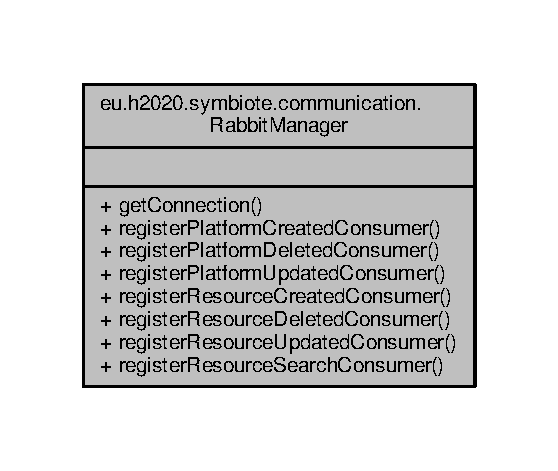
\includegraphics[width=268pt]{classeu_1_1h2020_1_1symbiote_1_1communication_1_1RabbitManager__coll__graph}
\end{center}
\end{figure}
\subsection*{Public Member Functions}
\begin{DoxyCompactItemize}
\item 
Connection {\bfseries get\+Connection} ()\hypertarget{classeu_1_1h2020_1_1symbiote_1_1communication_1_1RabbitManager_aa3cceb0c39fb9f29c209e228861c71f9}{}\label{classeu_1_1h2020_1_1symbiote_1_1communication_1_1RabbitManager_aa3cceb0c39fb9f29c209e228861c71f9}

\item 
void \hyperlink{classeu_1_1h2020_1_1symbiote_1_1communication_1_1RabbitManager_a7a6a139978888d37dca9e8c28302caf7}{register\+Platform\+Created\+Consumer} (\hyperlink{classeu_1_1h2020_1_1symbiote_1_1handlers_1_1PlatformHandler}{Platform\+Handler} platform\+Handler)  throws I\+O\+Exception 
\item 
void \hyperlink{classeu_1_1h2020_1_1symbiote_1_1communication_1_1RabbitManager_a3880a703e3565ec6e3e963bb12dcb172}{register\+Platform\+Deleted\+Consumer} (\hyperlink{classeu_1_1h2020_1_1symbiote_1_1handlers_1_1PlatformHandler}{Platform\+Handler} platform\+Handler)  throws I\+O\+Exception 
\item 
void \hyperlink{classeu_1_1h2020_1_1symbiote_1_1communication_1_1RabbitManager_a7ccf45180bab08a9a32b262f41705275}{register\+Platform\+Updated\+Consumer} (\hyperlink{classeu_1_1h2020_1_1symbiote_1_1handlers_1_1PlatformHandler}{Platform\+Handler} platform\+Handler)  throws I\+O\+Exception 
\item 
void \hyperlink{classeu_1_1h2020_1_1symbiote_1_1communication_1_1RabbitManager_a0ac5ce822697145440ae35bae985b813}{register\+Resource\+Created\+Consumer} (\hyperlink{classeu_1_1h2020_1_1symbiote_1_1handlers_1_1ResourceHandler}{Resource\+Handler} resource\+Handler)  throws I\+O\+Exception 
\item 
void \hyperlink{classeu_1_1h2020_1_1symbiote_1_1communication_1_1RabbitManager_aab1820f1814d33e13341d9fe98e74f2d}{register\+Resource\+Deleted\+Consumer} (\hyperlink{classeu_1_1h2020_1_1symbiote_1_1handlers_1_1ResourceHandler}{Resource\+Handler} resource\+Delete\+Handler)  throws I\+O\+Exception 
\item 
void \hyperlink{classeu_1_1h2020_1_1symbiote_1_1communication_1_1RabbitManager_a61d5f93decb2e133b040dd598f387c93}{register\+Resource\+Updated\+Consumer} (\hyperlink{classeu_1_1h2020_1_1symbiote_1_1handlers_1_1ResourceHandler}{Resource\+Handler} resource\+Handler)  throws I\+O\+Exception 
\item 
void \hyperlink{classeu_1_1h2020_1_1symbiote_1_1communication_1_1RabbitManager_a9693e85bfdfb097ef357ccbc8c3d8e8a}{register\+Resource\+Search\+Consumer} (\hyperlink{classeu_1_1h2020_1_1symbiote_1_1handlers_1_1SearchHandler}{Search\+Handler} search\+Handler)  throws I\+O\+Exception 
\end{DoxyCompactItemize}


\subsection{Detailed Description}
Bean used to manage internal communication using Rabbit\+MQ. It is responsible for declaring exchanges and using routing keys from centralized config server. 

\subsection{Member Function Documentation}
\index{eu\+::h2020\+::symbiote\+::communication\+::\+Rabbit\+Manager@{eu\+::h2020\+::symbiote\+::communication\+::\+Rabbit\+Manager}!register\+Platform\+Created\+Consumer@{register\+Platform\+Created\+Consumer}}
\index{register\+Platform\+Created\+Consumer@{register\+Platform\+Created\+Consumer}!eu\+::h2020\+::symbiote\+::communication\+::\+Rabbit\+Manager@{eu\+::h2020\+::symbiote\+::communication\+::\+Rabbit\+Manager}}
\subsubsection[{\texorpdfstring{register\+Platform\+Created\+Consumer(\+Platform\+Handler platform\+Handler)}{registerPlatformCreatedConsumer(PlatformHandler platformHandler)}}]{\setlength{\rightskip}{0pt plus 5cm}void eu.\+h2020.\+symbiote.\+communication.\+Rabbit\+Manager.\+register\+Platform\+Created\+Consumer (
\begin{DoxyParamCaption}
\item[{{\bf Platform\+Handler}}]{platform\+Handler}
\end{DoxyParamCaption}
) throws I\+O\+Exception}\hypertarget{classeu_1_1h2020_1_1symbiote_1_1communication_1_1RabbitManager_a7a6a139978888d37dca9e8c28302caf7}{}\label{classeu_1_1h2020_1_1symbiote_1_1communication_1_1RabbitManager_a7a6a139978888d37dca9e8c28302caf7}
Registers consumer for event platform.\+created. Event will trigger translation of the platform into R\+DF and writing it into J\+E\+NA repository.


\begin{DoxyParams}{Parameters}
{\em platform\+Handler} & Event handler which will be triggered when platform.\+created event is received. \\
\hline
\end{DoxyParams}

\begin{DoxyExceptions}{Exceptions}
{\em I\+O\+Exception} & In case there are problems with Rabbit\+MQ connections. \\
\hline
\end{DoxyExceptions}
\index{eu\+::h2020\+::symbiote\+::communication\+::\+Rabbit\+Manager@{eu\+::h2020\+::symbiote\+::communication\+::\+Rabbit\+Manager}!register\+Platform\+Deleted\+Consumer@{register\+Platform\+Deleted\+Consumer}}
\index{register\+Platform\+Deleted\+Consumer@{register\+Platform\+Deleted\+Consumer}!eu\+::h2020\+::symbiote\+::communication\+::\+Rabbit\+Manager@{eu\+::h2020\+::symbiote\+::communication\+::\+Rabbit\+Manager}}
\subsubsection[{\texorpdfstring{register\+Platform\+Deleted\+Consumer(\+Platform\+Handler platform\+Handler)}{registerPlatformDeletedConsumer(PlatformHandler platformHandler)}}]{\setlength{\rightskip}{0pt plus 5cm}void eu.\+h2020.\+symbiote.\+communication.\+Rabbit\+Manager.\+register\+Platform\+Deleted\+Consumer (
\begin{DoxyParamCaption}
\item[{{\bf Platform\+Handler}}]{platform\+Handler}
\end{DoxyParamCaption}
) throws I\+O\+Exception}\hypertarget{classeu_1_1h2020_1_1symbiote_1_1communication_1_1RabbitManager_a3880a703e3565ec6e3e963bb12dcb172}{}\label{classeu_1_1h2020_1_1symbiote_1_1communication_1_1RabbitManager_a3880a703e3565ec6e3e963bb12dcb172}
Registers consumer for event platform.\+deleted. Event will trigger translation of the request into S\+P\+A\+R\+QL U\+P\+D\+A\+TE and executing it in J\+E\+NA repository.


\begin{DoxyParams}{Parameters}
{\em platform\+Handler} & Event handler which will be triggered when platform.\+deleted event is received. \\
\hline
\end{DoxyParams}

\begin{DoxyExceptions}{Exceptions}
{\em I\+O\+Exception} & In case there are problems with Rabbit\+MQ connections. \\
\hline
\end{DoxyExceptions}
\index{eu\+::h2020\+::symbiote\+::communication\+::\+Rabbit\+Manager@{eu\+::h2020\+::symbiote\+::communication\+::\+Rabbit\+Manager}!register\+Platform\+Updated\+Consumer@{register\+Platform\+Updated\+Consumer}}
\index{register\+Platform\+Updated\+Consumer@{register\+Platform\+Updated\+Consumer}!eu\+::h2020\+::symbiote\+::communication\+::\+Rabbit\+Manager@{eu\+::h2020\+::symbiote\+::communication\+::\+Rabbit\+Manager}}
\subsubsection[{\texorpdfstring{register\+Platform\+Updated\+Consumer(\+Platform\+Handler platform\+Handler)}{registerPlatformUpdatedConsumer(PlatformHandler platformHandler)}}]{\setlength{\rightskip}{0pt plus 5cm}void eu.\+h2020.\+symbiote.\+communication.\+Rabbit\+Manager.\+register\+Platform\+Updated\+Consumer (
\begin{DoxyParamCaption}
\item[{{\bf Platform\+Handler}}]{platform\+Handler}
\end{DoxyParamCaption}
) throws I\+O\+Exception}\hypertarget{classeu_1_1h2020_1_1symbiote_1_1communication_1_1RabbitManager_a7ccf45180bab08a9a32b262f41705275}{}\label{classeu_1_1h2020_1_1symbiote_1_1communication_1_1RabbitManager_a7ccf45180bab08a9a32b262f41705275}
Registers consumer for event platform.\+updated. Event will trigger translation of the resource into R\+DF and writing it into J\+E\+NA repository.


\begin{DoxyParams}{Parameters}
{\em platform\+Handler} & Event handler which will be triggered when platform.\+updated event is received. \\
\hline
\end{DoxyParams}

\begin{DoxyExceptions}{Exceptions}
{\em I\+O\+Exception} & In case there are problems with Rabbit\+MQ connections. \\
\hline
\end{DoxyExceptions}
\index{eu\+::h2020\+::symbiote\+::communication\+::\+Rabbit\+Manager@{eu\+::h2020\+::symbiote\+::communication\+::\+Rabbit\+Manager}!register\+Resource\+Created\+Consumer@{register\+Resource\+Created\+Consumer}}
\index{register\+Resource\+Created\+Consumer@{register\+Resource\+Created\+Consumer}!eu\+::h2020\+::symbiote\+::communication\+::\+Rabbit\+Manager@{eu\+::h2020\+::symbiote\+::communication\+::\+Rabbit\+Manager}}
\subsubsection[{\texorpdfstring{register\+Resource\+Created\+Consumer(\+Resource\+Handler resource\+Handler)}{registerResourceCreatedConsumer(ResourceHandler resourceHandler)}}]{\setlength{\rightskip}{0pt plus 5cm}void eu.\+h2020.\+symbiote.\+communication.\+Rabbit\+Manager.\+register\+Resource\+Created\+Consumer (
\begin{DoxyParamCaption}
\item[{{\bf Resource\+Handler}}]{resource\+Handler}
\end{DoxyParamCaption}
) throws I\+O\+Exception}\hypertarget{classeu_1_1h2020_1_1symbiote_1_1communication_1_1RabbitManager_a0ac5ce822697145440ae35bae985b813}{}\label{classeu_1_1h2020_1_1symbiote_1_1communication_1_1RabbitManager_a0ac5ce822697145440ae35bae985b813}
Registers consumer for event resource.\+created. Event will trigger translation of the resource into R\+DF and writing it into J\+E\+NA repository.


\begin{DoxyParams}{Parameters}
{\em resource\+Handler} & Event handler which will be triggered when resource.\+created event is received. \\
\hline
\end{DoxyParams}

\begin{DoxyExceptions}{Exceptions}
{\em I\+O\+Exception} & In case there are problems with Rabbit\+MQ connections. \\
\hline
\end{DoxyExceptions}
\index{eu\+::h2020\+::symbiote\+::communication\+::\+Rabbit\+Manager@{eu\+::h2020\+::symbiote\+::communication\+::\+Rabbit\+Manager}!register\+Resource\+Deleted\+Consumer@{register\+Resource\+Deleted\+Consumer}}
\index{register\+Resource\+Deleted\+Consumer@{register\+Resource\+Deleted\+Consumer}!eu\+::h2020\+::symbiote\+::communication\+::\+Rabbit\+Manager@{eu\+::h2020\+::symbiote\+::communication\+::\+Rabbit\+Manager}}
\subsubsection[{\texorpdfstring{register\+Resource\+Deleted\+Consumer(\+Resource\+Handler resource\+Delete\+Handler)}{registerResourceDeletedConsumer(ResourceHandler resourceDeleteHandler)}}]{\setlength{\rightskip}{0pt plus 5cm}void eu.\+h2020.\+symbiote.\+communication.\+Rabbit\+Manager.\+register\+Resource\+Deleted\+Consumer (
\begin{DoxyParamCaption}
\item[{{\bf Resource\+Handler}}]{resource\+Delete\+Handler}
\end{DoxyParamCaption}
) throws I\+O\+Exception}\hypertarget{classeu_1_1h2020_1_1symbiote_1_1communication_1_1RabbitManager_aab1820f1814d33e13341d9fe98e74f2d}{}\label{classeu_1_1h2020_1_1symbiote_1_1communication_1_1RabbitManager_aab1820f1814d33e13341d9fe98e74f2d}
Registers consumer for event resource.\+deleted. Event will trigger translation of the request into S\+P\+A\+R\+QL U\+P\+D\+A\+TE and executing it in J\+E\+NA repository.


\begin{DoxyParams}{Parameters}
{\em resource\+Delete\+Handler} & Event handler which will be triggered when resource.\+deleted event is received. \\
\hline
\end{DoxyParams}

\begin{DoxyExceptions}{Exceptions}
{\em I\+O\+Exception} & In case there are problems with Rabbit\+MQ connections. \\
\hline
\end{DoxyExceptions}
\index{eu\+::h2020\+::symbiote\+::communication\+::\+Rabbit\+Manager@{eu\+::h2020\+::symbiote\+::communication\+::\+Rabbit\+Manager}!register\+Resource\+Search\+Consumer@{register\+Resource\+Search\+Consumer}}
\index{register\+Resource\+Search\+Consumer@{register\+Resource\+Search\+Consumer}!eu\+::h2020\+::symbiote\+::communication\+::\+Rabbit\+Manager@{eu\+::h2020\+::symbiote\+::communication\+::\+Rabbit\+Manager}}
\subsubsection[{\texorpdfstring{register\+Resource\+Search\+Consumer(\+Search\+Handler search\+Handler)}{registerResourceSearchConsumer(SearchHandler searchHandler)}}]{\setlength{\rightskip}{0pt plus 5cm}void eu.\+h2020.\+symbiote.\+communication.\+Rabbit\+Manager.\+register\+Resource\+Search\+Consumer (
\begin{DoxyParamCaption}
\item[{{\bf Search\+Handler}}]{search\+Handler}
\end{DoxyParamCaption}
) throws I\+O\+Exception}\hypertarget{classeu_1_1h2020_1_1symbiote_1_1communication_1_1RabbitManager_a9693e85bfdfb097ef357ccbc8c3d8e8a}{}\label{classeu_1_1h2020_1_1symbiote_1_1communication_1_1RabbitManager_a9693e85bfdfb097ef357ccbc8c3d8e8a}
Registers consumer for event resource.\+search\+Requested. Event will trigger translation of the request into S\+P\+A\+R\+QL and executing it in J\+E\+NA repository.


\begin{DoxyParams}{Parameters}
{\em search\+Handler} & Event handler which will be triggered when resource.\+search\+Requested event is received. \\
\hline
\end{DoxyParams}

\begin{DoxyExceptions}{Exceptions}
{\em I\+O\+Exception} & In case there are problems with Rabbit\+MQ connections. \\
\hline
\end{DoxyExceptions}
\index{eu\+::h2020\+::symbiote\+::communication\+::\+Rabbit\+Manager@{eu\+::h2020\+::symbiote\+::communication\+::\+Rabbit\+Manager}!register\+Resource\+Updated\+Consumer@{register\+Resource\+Updated\+Consumer}}
\index{register\+Resource\+Updated\+Consumer@{register\+Resource\+Updated\+Consumer}!eu\+::h2020\+::symbiote\+::communication\+::\+Rabbit\+Manager@{eu\+::h2020\+::symbiote\+::communication\+::\+Rabbit\+Manager}}
\subsubsection[{\texorpdfstring{register\+Resource\+Updated\+Consumer(\+Resource\+Handler resource\+Handler)}{registerResourceUpdatedConsumer(ResourceHandler resourceHandler)}}]{\setlength{\rightskip}{0pt plus 5cm}void eu.\+h2020.\+symbiote.\+communication.\+Rabbit\+Manager.\+register\+Resource\+Updated\+Consumer (
\begin{DoxyParamCaption}
\item[{{\bf Resource\+Handler}}]{resource\+Handler}
\end{DoxyParamCaption}
) throws I\+O\+Exception}\hypertarget{classeu_1_1h2020_1_1symbiote_1_1communication_1_1RabbitManager_a61d5f93decb2e133b040dd598f387c93}{}\label{classeu_1_1h2020_1_1symbiote_1_1communication_1_1RabbitManager_a61d5f93decb2e133b040dd598f387c93}
Registers consumer for event resource.\+created. Event will trigger translation of the resource into R\+DF and writing it into J\+E\+NA repository.


\begin{DoxyParams}{Parameters}
{\em resource\+Handler} & Event handler which will be triggered when resource.\+created event is received. \\
\hline
\end{DoxyParams}

\begin{DoxyExceptions}{Exceptions}
{\em I\+O\+Exception} & In case there are problems with Rabbit\+MQ connections. \\
\hline
\end{DoxyExceptions}


The documentation for this class was generated from the following file\+:\begin{DoxyCompactItemize}
\item 
src/main/java/eu/h2020/symbiote/communication/Rabbit\+Manager.\+java\end{DoxyCompactItemize}

\hypertarget{enumeu_1_1h2020_1_1symbiote_1_1ontology_1_1model_1_1RDFFormat}{}\section{eu.\+h2020.\+symbiote.\+ontology.\+model.\+R\+D\+F\+Format Enum Reference}
\label{enumeu_1_1h2020_1_1symbiote_1_1ontology_1_1model_1_1RDFFormat}\index{eu.\+h2020.\+symbiote.\+ontology.\+model.\+R\+D\+F\+Format@{eu.\+h2020.\+symbiote.\+ontology.\+model.\+R\+D\+F\+Format}}


Collaboration diagram for eu.\+h2020.\+symbiote.\+ontology.\+model.\+R\+D\+F\+Format\+:
\nopagebreak
\begin{figure}[H]
\begin{center}
\leavevmode
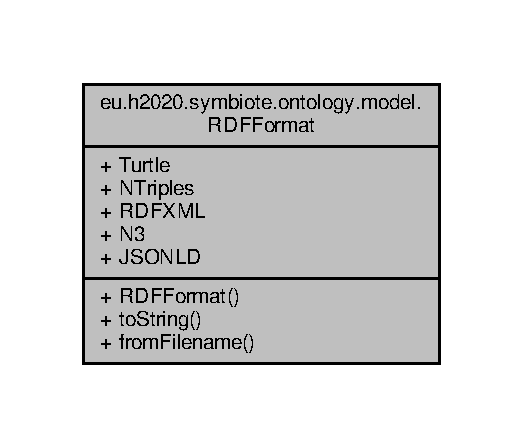
\includegraphics[width=251pt]{enumeu_1_1h2020_1_1symbiote_1_1ontology_1_1model_1_1RDFFormat__coll__graph}
\end{center}
\end{figure}
\subsection*{Public Member Functions}
\begin{DoxyCompactItemize}
\item 
{\bfseries R\+D\+F\+Format} (String name)\hypertarget{enumeu_1_1h2020_1_1symbiote_1_1ontology_1_1model_1_1RDFFormat_a6e3856212c9f3a5cb7fbf14f3524ceac}{}\label{enumeu_1_1h2020_1_1symbiote_1_1ontology_1_1model_1_1RDFFormat_a6e3856212c9f3a5cb7fbf14f3524ceac}

\item 
String {\bfseries to\+String} ()\hypertarget{enumeu_1_1h2020_1_1symbiote_1_1ontology_1_1model_1_1RDFFormat_a698b28158da86bc030351d3ce91ab5e5}{}\label{enumeu_1_1h2020_1_1symbiote_1_1ontology_1_1model_1_1RDFFormat_a698b28158da86bc030351d3ce91ab5e5}

\end{DoxyCompactItemize}
\subsection*{Static Public Member Functions}
\begin{DoxyCompactItemize}
\item 
static \hyperlink{enumeu_1_1h2020_1_1symbiote_1_1ontology_1_1model_1_1RDFFormat}{R\+D\+F\+Format} {\bfseries from\+Filename} (String filename)\hypertarget{enumeu_1_1h2020_1_1symbiote_1_1ontology_1_1model_1_1RDFFormat_a865345942ea348992c8fc1129a654772}{}\label{enumeu_1_1h2020_1_1symbiote_1_1ontology_1_1model_1_1RDFFormat_a865345942ea348992c8fc1129a654772}

\end{DoxyCompactItemize}
\subsection*{Public Attributes}
\begin{DoxyCompactItemize}
\item 
{\bfseries Turtle} =(\char`\"{}T\+U\+R\+T\+LE\char`\"{})\hypertarget{enumeu_1_1h2020_1_1symbiote_1_1ontology_1_1model_1_1RDFFormat_ab2fc0194cb2fae24cb4ef442b57e1ad0}{}\label{enumeu_1_1h2020_1_1symbiote_1_1ontology_1_1model_1_1RDFFormat_ab2fc0194cb2fae24cb4ef442b57e1ad0}

\item 
{\bfseries N\+Triples} =(\char`\"{}N\+T\+R\+I\+P\+L\+ES\char`\"{})\hypertarget{enumeu_1_1h2020_1_1symbiote_1_1ontology_1_1model_1_1RDFFormat_a90e0cd43f13667dd67b641d102e01010}{}\label{enumeu_1_1h2020_1_1symbiote_1_1ontology_1_1model_1_1RDFFormat_a90e0cd43f13667dd67b641d102e01010}

\item 
{\bfseries R\+D\+F\+X\+ML} =(\char`\"{}R\+D\+F\+X\+ML\char`\"{})\hypertarget{enumeu_1_1h2020_1_1symbiote_1_1ontology_1_1model_1_1RDFFormat_ab69c58ec5cd51cc35eee3612f3a8a7f0}{}\label{enumeu_1_1h2020_1_1symbiote_1_1ontology_1_1model_1_1RDFFormat_ab69c58ec5cd51cc35eee3612f3a8a7f0}

\item 
{\bfseries N3} =(\char`\"{}N3\char`\"{})\hypertarget{enumeu_1_1h2020_1_1symbiote_1_1ontology_1_1model_1_1RDFFormat_afa7e4a7139033f31bbea9130c569fff8}{}\label{enumeu_1_1h2020_1_1symbiote_1_1ontology_1_1model_1_1RDFFormat_afa7e4a7139033f31bbea9130c569fff8}

\item 
{\bfseries J\+S\+O\+N\+LD} =(\char`\"{}J\+S\+O\+N\+LD\char`\"{})\hypertarget{enumeu_1_1h2020_1_1symbiote_1_1ontology_1_1model_1_1RDFFormat_af64123c7a90b909a256ed0dcd63b2998}{}\label{enumeu_1_1h2020_1_1symbiote_1_1ontology_1_1model_1_1RDFFormat_af64123c7a90b909a256ed0dcd63b2998}

\end{DoxyCompactItemize}


\subsection{Detailed Description}
Enum containing possible R\+DF formats and their extensions.

\begin{DoxyAuthor}{Author}
jab 
\end{DoxyAuthor}


The documentation for this enum was generated from the following file\+:\begin{DoxyCompactItemize}
\item 
src/main/java/eu/h2020/symbiote/ontology/model/R\+D\+F\+Format.\+java\end{DoxyCompactItemize}

\hypertarget{classeu_1_1h2020_1_1symbiote_1_1ontology_1_1model_1_1Registry}{}\section{eu.\+h2020.\+symbiote.\+ontology.\+model.\+Registry Class Reference}
\label{classeu_1_1h2020_1_1symbiote_1_1ontology_1_1model_1_1Registry}\index{eu.\+h2020.\+symbiote.\+ontology.\+model.\+Registry@{eu.\+h2020.\+symbiote.\+ontology.\+model.\+Registry}}


Collaboration diagram for eu.\+h2020.\+symbiote.\+ontology.\+model.\+Registry\+:
\nopagebreak
\begin{figure}[H]
\begin{center}
\leavevmode
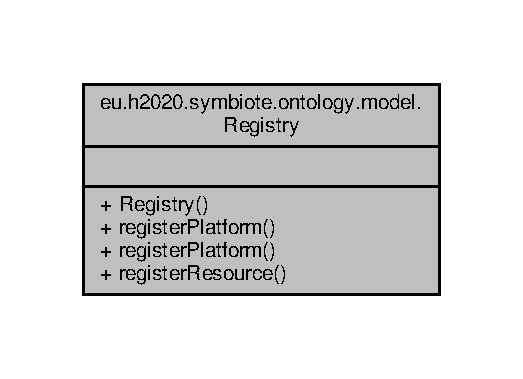
\includegraphics[width=251pt]{classeu_1_1h2020_1_1symbiote_1_1ontology_1_1model_1_1Registry__coll__graph}
\end{center}
\end{figure}
\subsection*{Public Member Functions}
\begin{DoxyCompactItemize}
\item 
{\bfseries Registry} (\hyperlink{classeu_1_1h2020_1_1symbiote_1_1ontology_1_1model_1_1TripleStore}{Triple\+Store} triple\+Store)\hypertarget{classeu_1_1h2020_1_1symbiote_1_1ontology_1_1model_1_1Registry_adcb1239b65bdcd80fb3fec88faa9fcb6}{}\label{classeu_1_1h2020_1_1symbiote_1_1ontology_1_1model_1_1Registry_adcb1239b65bdcd80fb3fec88faa9fcb6}

\item 
void {\bfseries register\+Platform} (String platform\+Id, String rdf, \hyperlink{enumeu_1_1h2020_1_1symbiote_1_1ontology_1_1model_1_1RDFFormat}{R\+D\+F\+Format} format, String model\+Id)\hypertarget{classeu_1_1h2020_1_1symbiote_1_1ontology_1_1model_1_1Registry_aba2012524676d2d17db541224e3e1183}{}\label{classeu_1_1h2020_1_1symbiote_1_1ontology_1_1model_1_1Registry_aba2012524676d2d17db541224e3e1183}

\item 
void {\bfseries register\+Platform} (String platform\+Id, Model rdf, String model\+Id)\hypertarget{classeu_1_1h2020_1_1symbiote_1_1ontology_1_1model_1_1Registry_a894d145edea63836ff08ab1d05cc07da}{}\label{classeu_1_1h2020_1_1symbiote_1_1ontology_1_1model_1_1Registry_a894d145edea63836ff08ab1d05cc07da}

\item 
void \hyperlink{classeu_1_1h2020_1_1symbiote_1_1ontology_1_1model_1_1Registry_a0f3f23b348b9033439e8553a4522b8a8}{register\+Resource} (String platform\+Uri, String service\+U\+RI, String resource\+Uri, Model resource\+Model)
\end{DoxyCompactItemize}


\subsection{Detailed Description}
\begin{DoxyAuthor}{Author}
jab 
\end{DoxyAuthor}


\subsection{Member Function Documentation}
\index{eu\+::h2020\+::symbiote\+::ontology\+::model\+::\+Registry@{eu\+::h2020\+::symbiote\+::ontology\+::model\+::\+Registry}!register\+Resource@{register\+Resource}}
\index{register\+Resource@{register\+Resource}!eu\+::h2020\+::symbiote\+::ontology\+::model\+::\+Registry@{eu\+::h2020\+::symbiote\+::ontology\+::model\+::\+Registry}}
\subsubsection[{\texorpdfstring{register\+Resource(\+String platform\+Uri, String service\+U\+R\+I, String resource\+Uri, Model resource\+Model)}{registerResource(String platformUri, String serviceURI, String resourceUri, Model resourceModel)}}]{\setlength{\rightskip}{0pt plus 5cm}void eu.\+h2020.\+symbiote.\+ontology.\+model.\+Registry.\+register\+Resource (
\begin{DoxyParamCaption}
\item[{String}]{platform\+Uri, }
\item[{String}]{service\+U\+RI, }
\item[{String}]{resource\+Uri, }
\item[{Model}]{resource\+Model}
\end{DoxyParamCaption}
)}\hypertarget{classeu_1_1h2020_1_1symbiote_1_1ontology_1_1model_1_1Registry_a0f3f23b348b9033439e8553a4522b8a8}{}\label{classeu_1_1h2020_1_1symbiote_1_1ontology_1_1model_1_1Registry_a0f3f23b348b9033439e8553a4522b8a8}
Registers resource of the platform described by specified Uri. Model will be stored in the platform\textquotesingle{}s named graph.


\begin{DoxyParams}{Parameters}
{\em platform\+Uri} & Uri of the platform for which resource is added. \\
\hline
{\em resource\+Model} & Model describiding the resource. \\
\hline
\end{DoxyParams}


The documentation for this class was generated from the following file\+:\begin{DoxyCompactItemize}
\item 
src/main/java/eu/h2020/symbiote/ontology/model/Registry.\+java\end{DoxyCompactItemize}

\hypertarget{classeu_1_1h2020_1_1symbiote_1_1model_1_1Resource}{}\section{eu.\+h2020.\+symbiote.\+model.\+Resource Class Reference}
\label{classeu_1_1h2020_1_1symbiote_1_1model_1_1Resource}\index{eu.\+h2020.\+symbiote.\+model.\+Resource@{eu.\+h2020.\+symbiote.\+model.\+Resource}}


Collaboration diagram for eu.\+h2020.\+symbiote.\+model.\+Resource\+:
\nopagebreak
\begin{figure}[H]
\begin{center}
\leavevmode
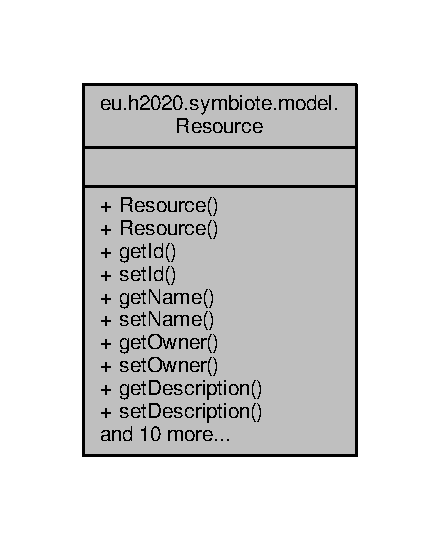
\includegraphics[width=211pt]{classeu_1_1h2020_1_1symbiote_1_1model_1_1Resource__coll__graph}
\end{center}
\end{figure}
\subsection*{Public Member Functions}
\begin{DoxyCompactItemize}
\item 
{\bfseries Resource} (String id, String name, String owner, String description, List$<$ String $>$ observed\+Properties, String resource\+U\+RL, \hyperlink{classeu_1_1h2020_1_1symbiote_1_1model_1_1Location}{Location} location, String feature\+Of\+Interest, String platform\+Id)\hypertarget{classeu_1_1h2020_1_1symbiote_1_1model_1_1Resource_a54cec3d9d4978f1457b601258ba78b0d}{}\label{classeu_1_1h2020_1_1symbiote_1_1model_1_1Resource_a54cec3d9d4978f1457b601258ba78b0d}

\item 
String {\bfseries get\+Id} ()\hypertarget{classeu_1_1h2020_1_1symbiote_1_1model_1_1Resource_a6d2b00f0e94b55cce1daff002012369c}{}\label{classeu_1_1h2020_1_1symbiote_1_1model_1_1Resource_a6d2b00f0e94b55cce1daff002012369c}

\item 
void {\bfseries set\+Id} (String id)\hypertarget{classeu_1_1h2020_1_1symbiote_1_1model_1_1Resource_a209815ba7cdb6b82334e664eb4c38708}{}\label{classeu_1_1h2020_1_1symbiote_1_1model_1_1Resource_a209815ba7cdb6b82334e664eb4c38708}

\item 
String {\bfseries get\+Name} ()\hypertarget{classeu_1_1h2020_1_1symbiote_1_1model_1_1Resource_a7332986d4dfa4ca233f705659f166f2c}{}\label{classeu_1_1h2020_1_1symbiote_1_1model_1_1Resource_a7332986d4dfa4ca233f705659f166f2c}

\item 
void {\bfseries set\+Name} (String name)\hypertarget{classeu_1_1h2020_1_1symbiote_1_1model_1_1Resource_ad2cd06bcbfa928adead9017509cc2e78}{}\label{classeu_1_1h2020_1_1symbiote_1_1model_1_1Resource_ad2cd06bcbfa928adead9017509cc2e78}

\item 
String {\bfseries get\+Owner} ()\hypertarget{classeu_1_1h2020_1_1symbiote_1_1model_1_1Resource_a0bd495e4c9a10fac6e885de268b5ad76}{}\label{classeu_1_1h2020_1_1symbiote_1_1model_1_1Resource_a0bd495e4c9a10fac6e885de268b5ad76}

\item 
void {\bfseries set\+Owner} (String owner)\hypertarget{classeu_1_1h2020_1_1symbiote_1_1model_1_1Resource_a4391365a9ef765fb9c96e8243a45fafb}{}\label{classeu_1_1h2020_1_1symbiote_1_1model_1_1Resource_a4391365a9ef765fb9c96e8243a45fafb}

\item 
String {\bfseries get\+Description} ()\hypertarget{classeu_1_1h2020_1_1symbiote_1_1model_1_1Resource_ae2ce583e094c18bca236027602739049}{}\label{classeu_1_1h2020_1_1symbiote_1_1model_1_1Resource_ae2ce583e094c18bca236027602739049}

\item 
void {\bfseries set\+Description} (String description)\hypertarget{classeu_1_1h2020_1_1symbiote_1_1model_1_1Resource_a19349909b51f43be943fcc3ebc078009}{}\label{classeu_1_1h2020_1_1symbiote_1_1model_1_1Resource_a19349909b51f43be943fcc3ebc078009}

\item 
List$<$ String $>$ {\bfseries get\+Observed\+Properties} ()\hypertarget{classeu_1_1h2020_1_1symbiote_1_1model_1_1Resource_a2aaf59e1be5b0c974a31e106adfa6c43}{}\label{classeu_1_1h2020_1_1symbiote_1_1model_1_1Resource_a2aaf59e1be5b0c974a31e106adfa6c43}

\item 
void {\bfseries set\+Observed\+Properties} (List$<$ String $>$ observed\+Properties)\hypertarget{classeu_1_1h2020_1_1symbiote_1_1model_1_1Resource_a826dbee60cf539ffbf1a088496ac7e11}{}\label{classeu_1_1h2020_1_1symbiote_1_1model_1_1Resource_a826dbee60cf539ffbf1a088496ac7e11}

\item 
String {\bfseries get\+Resource\+U\+RL} ()\hypertarget{classeu_1_1h2020_1_1symbiote_1_1model_1_1Resource_a4a0c05d9007f2216c55ddc32a44f467b}{}\label{classeu_1_1h2020_1_1symbiote_1_1model_1_1Resource_a4a0c05d9007f2216c55ddc32a44f467b}

\item 
void {\bfseries set\+Resource\+U\+RL} (String resource\+U\+RL)\hypertarget{classeu_1_1h2020_1_1symbiote_1_1model_1_1Resource_a27d7401a8087bf902fd575039d574d0c}{}\label{classeu_1_1h2020_1_1symbiote_1_1model_1_1Resource_a27d7401a8087bf902fd575039d574d0c}

\item 
\hyperlink{classeu_1_1h2020_1_1symbiote_1_1model_1_1Location}{Location} {\bfseries get\+Location} ()\hypertarget{classeu_1_1h2020_1_1symbiote_1_1model_1_1Resource_acfb7ead093f1ed692640c99daba8fc6c}{}\label{classeu_1_1h2020_1_1symbiote_1_1model_1_1Resource_acfb7ead093f1ed692640c99daba8fc6c}

\item 
void {\bfseries set\+Location} (\hyperlink{classeu_1_1h2020_1_1symbiote_1_1model_1_1Location}{Location} location)\hypertarget{classeu_1_1h2020_1_1symbiote_1_1model_1_1Resource_a14eba3bd0171783f32d6d4446768905d}{}\label{classeu_1_1h2020_1_1symbiote_1_1model_1_1Resource_a14eba3bd0171783f32d6d4446768905d}

\item 
String {\bfseries get\+Feature\+Of\+Interest} ()\hypertarget{classeu_1_1h2020_1_1symbiote_1_1model_1_1Resource_a1e5912a2e60f0d2dcda674f26ebe871b}{}\label{classeu_1_1h2020_1_1symbiote_1_1model_1_1Resource_a1e5912a2e60f0d2dcda674f26ebe871b}

\item 
void {\bfseries set\+Feature\+Of\+Interest} (String feature\+Of\+Interest)\hypertarget{classeu_1_1h2020_1_1symbiote_1_1model_1_1Resource_abcfd5b3b2e1515ca7e9eb50eeb7ed0cf}{}\label{classeu_1_1h2020_1_1symbiote_1_1model_1_1Resource_abcfd5b3b2e1515ca7e9eb50eeb7ed0cf}

\item 
String {\bfseries get\+Platform\+Id} ()\hypertarget{classeu_1_1h2020_1_1symbiote_1_1model_1_1Resource_a97e847fb787ea9fe1d16d8bd702deece}{}\label{classeu_1_1h2020_1_1symbiote_1_1model_1_1Resource_a97e847fb787ea9fe1d16d8bd702deece}

\item 
void {\bfseries set\+Platform\+Id} (String platform\+Id)\hypertarget{classeu_1_1h2020_1_1symbiote_1_1model_1_1Resource_a4f3c37b066d6e6587912fa1f1240048f}{}\label{classeu_1_1h2020_1_1symbiote_1_1model_1_1Resource_a4f3c37b066d6e6587912fa1f1240048f}

\end{DoxyCompactItemize}


\subsection{Detailed Description}
Class representing resource object in the system events.

Created by Mael on 16/01/2017. 

The documentation for this class was generated from the following file\+:\begin{DoxyCompactItemize}
\item 
src/main/java/eu/h2020/symbiote/model/Resource.\+java\end{DoxyCompactItemize}

\hypertarget{classeu_1_1h2020_1_1symbiote_1_1query_1_1ResourceAndObservedPropertyQueryGenerator}{}\section{eu.\+h2020.\+symbiote.\+query.\+Resource\+And\+Observed\+Property\+Query\+Generator Class Reference}
\label{classeu_1_1h2020_1_1symbiote_1_1query_1_1ResourceAndObservedPropertyQueryGenerator}\index{eu.\+h2020.\+symbiote.\+query.\+Resource\+And\+Observed\+Property\+Query\+Generator@{eu.\+h2020.\+symbiote.\+query.\+Resource\+And\+Observed\+Property\+Query\+Generator}}


Collaboration diagram for eu.\+h2020.\+symbiote.\+query.\+Resource\+And\+Observed\+Property\+Query\+Generator\+:
\nopagebreak
\begin{figure}[H]
\begin{center}
\leavevmode
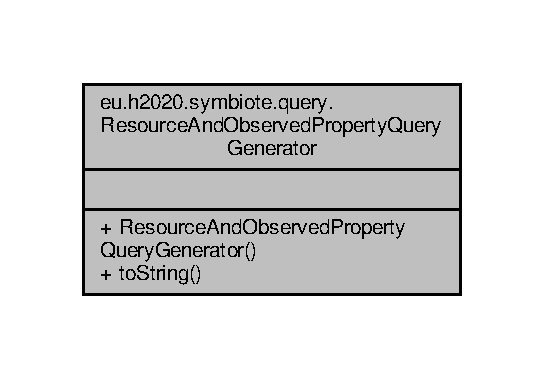
\includegraphics[width=261pt]{classeu_1_1h2020_1_1symbiote_1_1query_1_1ResourceAndObservedPropertyQueryGenerator__coll__graph}
\end{center}
\end{figure}
\subsection*{Public Member Functions}
\begin{DoxyCompactItemize}
\item 
{\bfseries Resource\+And\+Observed\+Property\+Query\+Generator} (String res\+Id)\hypertarget{classeu_1_1h2020_1_1symbiote_1_1query_1_1ResourceAndObservedPropertyQueryGenerator_a56889c8e719deac65e4b4b383c0429dd}{}\label{classeu_1_1h2020_1_1symbiote_1_1query_1_1ResourceAndObservedPropertyQueryGenerator_a56889c8e719deac65e4b4b383c0429dd}

\item 
String {\bfseries to\+String} ()\hypertarget{classeu_1_1h2020_1_1symbiote_1_1query_1_1ResourceAndObservedPropertyQueryGenerator_a5f8ee788f623760977f48e3788fdb0fd}{}\label{classeu_1_1h2020_1_1symbiote_1_1query_1_1ResourceAndObservedPropertyQueryGenerator_a5f8ee788f623760977f48e3788fdb0fd}

\end{DoxyCompactItemize}


\subsection{Detailed Description}
Created by Mael on 26/01/2017. 

The documentation for this class was generated from the following file\+:\begin{DoxyCompactItemize}
\item 
src/main/java/eu/h2020/symbiote/query/Resource\+And\+Observed\+Property\+Query\+Generator.\+java\end{DoxyCompactItemize}

\hypertarget{classeu_1_1h2020_1_1symbiote_1_1communication_1_1ResourceCreatedConsumer}{}\section{eu.\+h2020.\+symbiote.\+communication.\+Resource\+Created\+Consumer Class Reference}
\label{classeu_1_1h2020_1_1symbiote_1_1communication_1_1ResourceCreatedConsumer}\index{eu.\+h2020.\+symbiote.\+communication.\+Resource\+Created\+Consumer@{eu.\+h2020.\+symbiote.\+communication.\+Resource\+Created\+Consumer}}


Inheritance diagram for eu.\+h2020.\+symbiote.\+communication.\+Resource\+Created\+Consumer\+:
\nopagebreak
\begin{figure}[H]
\begin{center}
\leavevmode
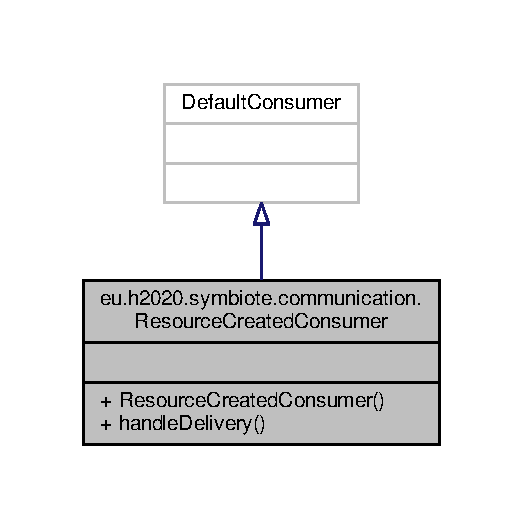
\includegraphics[width=251pt]{classeu_1_1h2020_1_1symbiote_1_1communication_1_1ResourceCreatedConsumer__inherit__graph}
\end{center}
\end{figure}


Collaboration diagram for eu.\+h2020.\+symbiote.\+communication.\+Resource\+Created\+Consumer\+:
\nopagebreak
\begin{figure}[H]
\begin{center}
\leavevmode
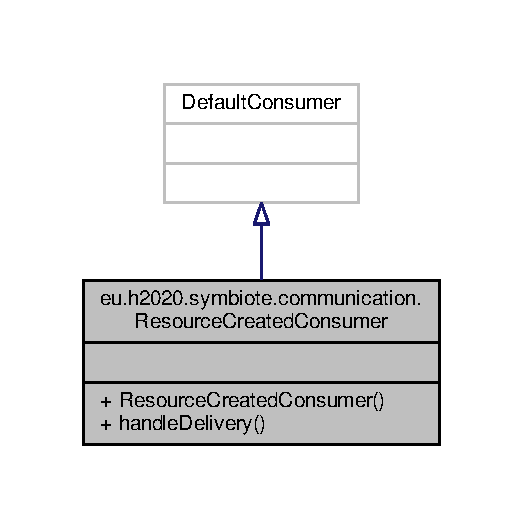
\includegraphics[width=251pt]{classeu_1_1h2020_1_1symbiote_1_1communication_1_1ResourceCreatedConsumer__coll__graph}
\end{center}
\end{figure}
\subsection*{Public Member Functions}
\begin{DoxyCompactItemize}
\item 
\hyperlink{classeu_1_1h2020_1_1symbiote_1_1communication_1_1ResourceCreatedConsumer_a02947dcf2a6ee894d265bd45fe4feefc}{Resource\+Created\+Consumer} (Channel channel, \hyperlink{classeu_1_1h2020_1_1symbiote_1_1handlers_1_1ResourceHandler}{Resource\+Handler} handler)
\item 
void {\bfseries handle\+Delivery} (String consumer\+Tag, Envelope envelope, A\+M\+Q\+P.\+Basic\+Properties properties, byte\mbox{[}$\,$\mbox{]} body)  throws I\+O\+Exception \hypertarget{classeu_1_1h2020_1_1symbiote_1_1communication_1_1ResourceCreatedConsumer_a4f7fbccebd994e942892f6621f61f909}{}\label{classeu_1_1h2020_1_1symbiote_1_1communication_1_1ResourceCreatedConsumer_a4f7fbccebd994e942892f6621f61f909}

\end{DoxyCompactItemize}


\subsection{Detailed Description}
Consumer of the resource created event. Handler creates R\+DF representation of provided resource and adds it into repository.

Created by Mael on 17/01/2017. 

\subsection{Constructor \& Destructor Documentation}
\index{eu\+::h2020\+::symbiote\+::communication\+::\+Resource\+Created\+Consumer@{eu\+::h2020\+::symbiote\+::communication\+::\+Resource\+Created\+Consumer}!Resource\+Created\+Consumer@{Resource\+Created\+Consumer}}
\index{Resource\+Created\+Consumer@{Resource\+Created\+Consumer}!eu\+::h2020\+::symbiote\+::communication\+::\+Resource\+Created\+Consumer@{eu\+::h2020\+::symbiote\+::communication\+::\+Resource\+Created\+Consumer}}
\subsubsection[{\texorpdfstring{Resource\+Created\+Consumer(\+Channel channel, Resource\+Handler handler)}{ResourceCreatedConsumer(Channel channel, ResourceHandler handler)}}]{\setlength{\rightskip}{0pt plus 5cm}eu.\+h2020.\+symbiote.\+communication.\+Resource\+Created\+Consumer.\+Resource\+Created\+Consumer (
\begin{DoxyParamCaption}
\item[{Channel}]{channel, }
\item[{{\bf Resource\+Handler}}]{handler}
\end{DoxyParamCaption}
)}\hypertarget{classeu_1_1h2020_1_1symbiote_1_1communication_1_1ResourceCreatedConsumer_a02947dcf2a6ee894d265bd45fe4feefc}{}\label{classeu_1_1h2020_1_1symbiote_1_1communication_1_1ResourceCreatedConsumer_a02947dcf2a6ee894d265bd45fe4feefc}
Constructs a new instance and records its association to the passed-\/in channel.


\begin{DoxyParams}{Parameters}
{\em channel} & the channel to which this consumer is attached \\
\hline
{\em handler} & handler to be used by the consumer. \\
\hline
\end{DoxyParams}


The documentation for this class was generated from the following file\+:\begin{DoxyCompactItemize}
\item 
src/main/java/eu/h2020/symbiote/communication/Resource\+Created\+Consumer.\+java\end{DoxyCompactItemize}

\hypertarget{classeu_1_1h2020_1_1symbiote_1_1communication_1_1ResourceDeletedConsumer}{}\section{eu.\+h2020.\+symbiote.\+communication.\+Resource\+Deleted\+Consumer Class Reference}
\label{classeu_1_1h2020_1_1symbiote_1_1communication_1_1ResourceDeletedConsumer}\index{eu.\+h2020.\+symbiote.\+communication.\+Resource\+Deleted\+Consumer@{eu.\+h2020.\+symbiote.\+communication.\+Resource\+Deleted\+Consumer}}


Inheritance diagram for eu.\+h2020.\+symbiote.\+communication.\+Resource\+Deleted\+Consumer\+:
\nopagebreak
\begin{figure}[H]
\begin{center}
\leavevmode
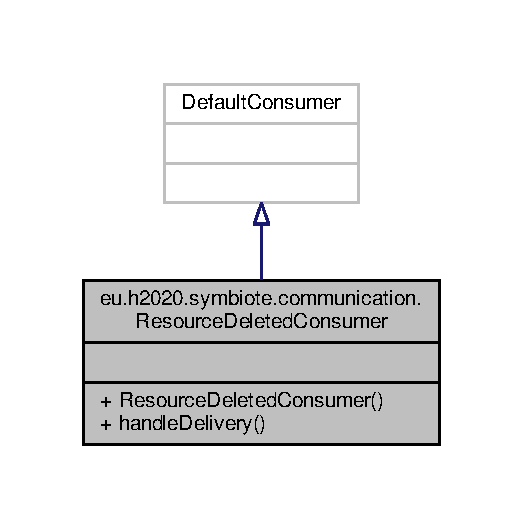
\includegraphics[width=251pt]{classeu_1_1h2020_1_1symbiote_1_1communication_1_1ResourceDeletedConsumer__inherit__graph}
\end{center}
\end{figure}


Collaboration diagram for eu.\+h2020.\+symbiote.\+communication.\+Resource\+Deleted\+Consumer\+:
\nopagebreak
\begin{figure}[H]
\begin{center}
\leavevmode
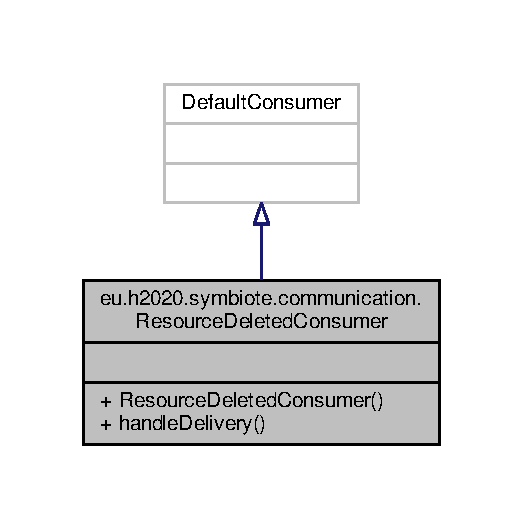
\includegraphics[width=251pt]{classeu_1_1h2020_1_1symbiote_1_1communication_1_1ResourceDeletedConsumer__coll__graph}
\end{center}
\end{figure}
\subsection*{Public Member Functions}
\begin{DoxyCompactItemize}
\item 
\hyperlink{classeu_1_1h2020_1_1symbiote_1_1communication_1_1ResourceDeletedConsumer_a916388b648d7332a81aeca3d7f546485}{Resource\+Deleted\+Consumer} (Channel channel, \hyperlink{classeu_1_1h2020_1_1symbiote_1_1handlers_1_1ResourceHandler}{Resource\+Handler} handler)
\item 
void {\bfseries handle\+Delivery} (String consumer\+Tag, Envelope envelope, A\+M\+Q\+P.\+Basic\+Properties properties, byte\mbox{[}$\,$\mbox{]} body)  throws I\+O\+Exception \hypertarget{classeu_1_1h2020_1_1symbiote_1_1communication_1_1ResourceDeletedConsumer_af0058d865f7a3fc2ab0813a5e14f6b17}{}\label{classeu_1_1h2020_1_1symbiote_1_1communication_1_1ResourceDeletedConsumer_af0058d865f7a3fc2ab0813a5e14f6b17}

\end{DoxyCompactItemize}


\subsection{Detailed Description}
Consumer of the search requested event. Translates the message as list of query parameters, translates them into S\+P\+A\+R\+QL and queries the repository.

Created by Mael on 17/01/2017. 

\subsection{Constructor \& Destructor Documentation}
\index{eu\+::h2020\+::symbiote\+::communication\+::\+Resource\+Deleted\+Consumer@{eu\+::h2020\+::symbiote\+::communication\+::\+Resource\+Deleted\+Consumer}!Resource\+Deleted\+Consumer@{Resource\+Deleted\+Consumer}}
\index{Resource\+Deleted\+Consumer@{Resource\+Deleted\+Consumer}!eu\+::h2020\+::symbiote\+::communication\+::\+Resource\+Deleted\+Consumer@{eu\+::h2020\+::symbiote\+::communication\+::\+Resource\+Deleted\+Consumer}}
\subsubsection[{\texorpdfstring{Resource\+Deleted\+Consumer(\+Channel channel, Resource\+Handler handler)}{ResourceDeletedConsumer(Channel channel, ResourceHandler handler)}}]{\setlength{\rightskip}{0pt plus 5cm}eu.\+h2020.\+symbiote.\+communication.\+Resource\+Deleted\+Consumer.\+Resource\+Deleted\+Consumer (
\begin{DoxyParamCaption}
\item[{Channel}]{channel, }
\item[{{\bf Resource\+Handler}}]{handler}
\end{DoxyParamCaption}
)}\hypertarget{classeu_1_1h2020_1_1symbiote_1_1communication_1_1ResourceDeletedConsumer_a916388b648d7332a81aeca3d7f546485}{}\label{classeu_1_1h2020_1_1symbiote_1_1communication_1_1ResourceDeletedConsumer_a916388b648d7332a81aeca3d7f546485}
Constructs a new instance and records its association to the passed-\/in channel.


\begin{DoxyParams}{Parameters}
{\em channel} & the channel to which this consumer is attached \\
\hline
{\em handler} & handler to be used by the consumer. \\
\hline
\end{DoxyParams}


The documentation for this class was generated from the following file\+:\begin{DoxyCompactItemize}
\item 
src/main/java/eu/h2020/symbiote/communication/Resource\+Deleted\+Consumer.\+java\end{DoxyCompactItemize}

\hypertarget{classeu_1_1h2020_1_1symbiote_1_1handlers_1_1ResourceHandler}{}\section{eu.\+h2020.\+symbiote.\+handlers.\+Resource\+Handler Class Reference}
\label{classeu_1_1h2020_1_1symbiote_1_1handlers_1_1ResourceHandler}\index{eu.\+h2020.\+symbiote.\+handlers.\+Resource\+Handler@{eu.\+h2020.\+symbiote.\+handlers.\+Resource\+Handler}}


Inheritance diagram for eu.\+h2020.\+symbiote.\+handlers.\+Resource\+Handler\+:
\nopagebreak
\begin{figure}[H]
\begin{center}
\leavevmode
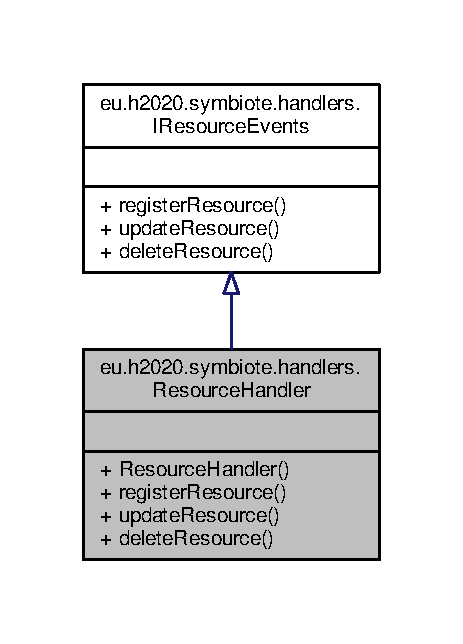
\includegraphics[width=222pt]{classeu_1_1h2020_1_1symbiote_1_1handlers_1_1ResourceHandler__inherit__graph}
\end{center}
\end{figure}


Collaboration diagram for eu.\+h2020.\+symbiote.\+handlers.\+Resource\+Handler\+:
\nopagebreak
\begin{figure}[H]
\begin{center}
\leavevmode
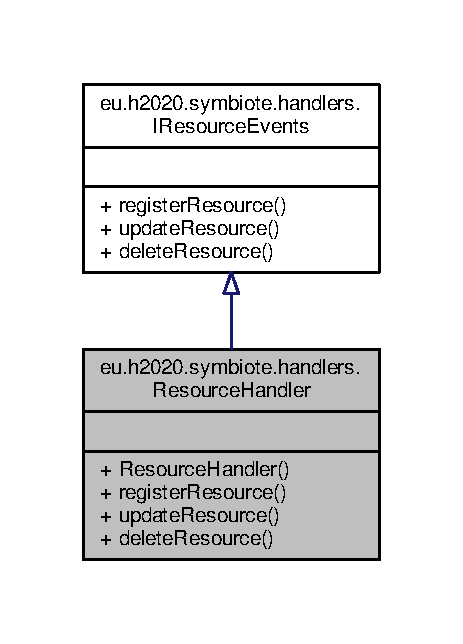
\includegraphics[width=222pt]{classeu_1_1h2020_1_1symbiote_1_1handlers_1_1ResourceHandler__coll__graph}
\end{center}
\end{figure}
\subsection*{Public Member Functions}
\begin{DoxyCompactItemize}
\item 
{\bfseries Resource\+Handler} (\hyperlink{classeu_1_1h2020_1_1symbiote_1_1search_1_1SearchStorage}{Search\+Storage} storage)\hypertarget{classeu_1_1h2020_1_1symbiote_1_1handlers_1_1ResourceHandler_a5e5b0f79d64c3938f9ca9a4e01a2385f}{}\label{classeu_1_1h2020_1_1symbiote_1_1handlers_1_1ResourceHandler_a5e5b0f79d64c3938f9ca9a4e01a2385f}

\item 
boolean \hyperlink{classeu_1_1h2020_1_1symbiote_1_1handlers_1_1ResourceHandler_ab1eb533aab8bcc871ce752edf66ecebd}{register\+Resource} (\hyperlink{classeu_1_1h2020_1_1symbiote_1_1model_1_1Resource}{Resource} resource)
\item 
boolean \hyperlink{classeu_1_1h2020_1_1symbiote_1_1handlers_1_1ResourceHandler_abeae05c859b45f15b818a6b6640e8ad1}{update\+Resource} (\hyperlink{classeu_1_1h2020_1_1symbiote_1_1model_1_1Resource}{Resource} resource)
\item 
boolean \hyperlink{classeu_1_1h2020_1_1symbiote_1_1handlers_1_1ResourceHandler_a549c5bae3e5502b436ba353ba8b39a25}{delete\+Resource} (String resource\+Id)
\end{DoxyCompactItemize}


\subsection{Detailed Description}
Created by Mael on 16/01/2017. 

\subsection{Member Function Documentation}
\index{eu\+::h2020\+::symbiote\+::handlers\+::\+Resource\+Handler@{eu\+::h2020\+::symbiote\+::handlers\+::\+Resource\+Handler}!delete\+Resource@{delete\+Resource}}
\index{delete\+Resource@{delete\+Resource}!eu\+::h2020\+::symbiote\+::handlers\+::\+Resource\+Handler@{eu\+::h2020\+::symbiote\+::handlers\+::\+Resource\+Handler}}
\subsubsection[{\texorpdfstring{delete\+Resource(\+String resource\+Id)}{deleteResource(String resourceId)}}]{\setlength{\rightskip}{0pt plus 5cm}boolean eu.\+h2020.\+symbiote.\+handlers.\+Resource\+Handler.\+delete\+Resource (
\begin{DoxyParamCaption}
\item[{String}]{resource\+Id}
\end{DoxyParamCaption}
)}\hypertarget{classeu_1_1h2020_1_1symbiote_1_1handlers_1_1ResourceHandler_a549c5bae3e5502b436ba353ba8b39a25}{}\label{classeu_1_1h2020_1_1symbiote_1_1handlers_1_1ResourceHandler_a549c5bae3e5502b436ba353ba8b39a25}
Deletes resource representation in the Apache Jena repository.


\begin{DoxyParams}{Parameters}
{\em resource\+Id} & Id of the resource to be deleted \\
\hline
\end{DoxyParams}
\begin{DoxyReturn}{Returns}
{\ttfamily true} if deletion was successful. 
\end{DoxyReturn}


Implements \hyperlink{interfaceeu_1_1h2020_1_1symbiote_1_1handlers_1_1IResourceEvents_a7c99a8192ec4b06735f641ae3cf2bd99}{eu.\+h2020.\+symbiote.\+handlers.\+I\+Resource\+Events}.

\index{eu\+::h2020\+::symbiote\+::handlers\+::\+Resource\+Handler@{eu\+::h2020\+::symbiote\+::handlers\+::\+Resource\+Handler}!register\+Resource@{register\+Resource}}
\index{register\+Resource@{register\+Resource}!eu\+::h2020\+::symbiote\+::handlers\+::\+Resource\+Handler@{eu\+::h2020\+::symbiote\+::handlers\+::\+Resource\+Handler}}
\subsubsection[{\texorpdfstring{register\+Resource(\+Resource resource)}{registerResource(Resource resource)}}]{\setlength{\rightskip}{0pt plus 5cm}boolean eu.\+h2020.\+symbiote.\+handlers.\+Resource\+Handler.\+register\+Resource (
\begin{DoxyParamCaption}
\item[{{\bf Resource}}]{resource}
\end{DoxyParamCaption}
)}\hypertarget{classeu_1_1h2020_1_1symbiote_1_1handlers_1_1ResourceHandler_ab1eb533aab8bcc871ce752edf66ecebd}{}\label{classeu_1_1h2020_1_1symbiote_1_1handlers_1_1ResourceHandler_ab1eb533aab8bcc871ce752edf66ecebd}
Registers resource representation in the Apache Jena repository.


\begin{DoxyParams}{Parameters}
{\em resource} & Resource to be saved \\
\hline
\end{DoxyParams}
\begin{DoxyReturn}{Returns}
{\ttfamily true} if registration was successful. 
\end{DoxyReturn}


Implements \hyperlink{interfaceeu_1_1h2020_1_1symbiote_1_1handlers_1_1IResourceEvents_a3941d9229b2efc8d5a80106e0ffe73cd}{eu.\+h2020.\+symbiote.\+handlers.\+I\+Resource\+Events}.

\index{eu\+::h2020\+::symbiote\+::handlers\+::\+Resource\+Handler@{eu\+::h2020\+::symbiote\+::handlers\+::\+Resource\+Handler}!update\+Resource@{update\+Resource}}
\index{update\+Resource@{update\+Resource}!eu\+::h2020\+::symbiote\+::handlers\+::\+Resource\+Handler@{eu\+::h2020\+::symbiote\+::handlers\+::\+Resource\+Handler}}
\subsubsection[{\texorpdfstring{update\+Resource(\+Resource resource)}{updateResource(Resource resource)}}]{\setlength{\rightskip}{0pt plus 5cm}boolean eu.\+h2020.\+symbiote.\+handlers.\+Resource\+Handler.\+update\+Resource (
\begin{DoxyParamCaption}
\item[{{\bf Resource}}]{resource}
\end{DoxyParamCaption}
)}\hypertarget{classeu_1_1h2020_1_1symbiote_1_1handlers_1_1ResourceHandler_abeae05c859b45f15b818a6b6640e8ad1}{}\label{classeu_1_1h2020_1_1symbiote_1_1handlers_1_1ResourceHandler_abeae05c859b45f15b818a6b6640e8ad1}
Updates specified resource representation in the Apache Jena repository.


\begin{DoxyParams}{Parameters}
{\em resource} & Updated resource \\
\hline
\end{DoxyParams}
\begin{DoxyReturn}{Returns}
{\ttfamily true} if update was successful. 
\end{DoxyReturn}


Implements \hyperlink{interfaceeu_1_1h2020_1_1symbiote_1_1handlers_1_1IResourceEvents_aaac836b0134ed41ad529b9ac3124a216}{eu.\+h2020.\+symbiote.\+handlers.\+I\+Resource\+Events}.



The documentation for this class was generated from the following file\+:\begin{DoxyCompactItemize}
\item 
src/main/java/eu/h2020/symbiote/handlers/Resource\+Handler.\+java\end{DoxyCompactItemize}

\hypertarget{classeu_1_1h2020_1_1symbiote_1_1communication_1_1ResourceModifiedConsumer}{}\section{eu.\+h2020.\+symbiote.\+communication.\+Resource\+Modified\+Consumer Class Reference}
\label{classeu_1_1h2020_1_1symbiote_1_1communication_1_1ResourceModifiedConsumer}\index{eu.\+h2020.\+symbiote.\+communication.\+Resource\+Modified\+Consumer@{eu.\+h2020.\+symbiote.\+communication.\+Resource\+Modified\+Consumer}}


Inheritance diagram for eu.\+h2020.\+symbiote.\+communication.\+Resource\+Modified\+Consumer\+:
\nopagebreak
\begin{figure}[H]
\begin{center}
\leavevmode
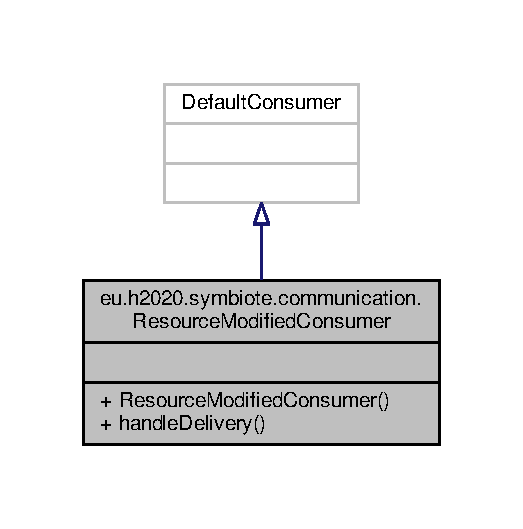
\includegraphics[width=251pt]{classeu_1_1h2020_1_1symbiote_1_1communication_1_1ResourceModifiedConsumer__inherit__graph}
\end{center}
\end{figure}


Collaboration diagram for eu.\+h2020.\+symbiote.\+communication.\+Resource\+Modified\+Consumer\+:
\nopagebreak
\begin{figure}[H]
\begin{center}
\leavevmode
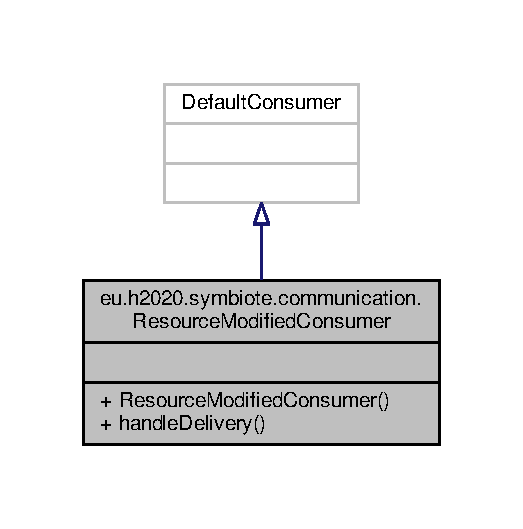
\includegraphics[width=251pt]{classeu_1_1h2020_1_1symbiote_1_1communication_1_1ResourceModifiedConsumer__coll__graph}
\end{center}
\end{figure}
\subsection*{Public Member Functions}
\begin{DoxyCompactItemize}
\item 
\hyperlink{classeu_1_1h2020_1_1symbiote_1_1communication_1_1ResourceModifiedConsumer_afd8d08311937404758901578724865c1}{Resource\+Modified\+Consumer} (Channel channel, \hyperlink{classeu_1_1h2020_1_1symbiote_1_1handlers_1_1ResourceHandler}{Resource\+Handler} handler)
\item 
void {\bfseries handle\+Delivery} (String consumer\+Tag, Envelope envelope, A\+M\+Q\+P.\+Basic\+Properties properties, byte\mbox{[}$\,$\mbox{]} body)  throws I\+O\+Exception \hypertarget{classeu_1_1h2020_1_1symbiote_1_1communication_1_1ResourceModifiedConsumer_aed5b3b33a3cbc85f4796da3cf869131e}{}\label{classeu_1_1h2020_1_1symbiote_1_1communication_1_1ResourceModifiedConsumer_aed5b3b33a3cbc85f4796da3cf869131e}

\end{DoxyCompactItemize}


\subsection{Detailed Description}
Consumer of the resource modified event. Handler removes existing resource and creates R\+DF representation of the new resource.

Created by Mael on 17/01/2017. 

\subsection{Constructor \& Destructor Documentation}
\index{eu\+::h2020\+::symbiote\+::communication\+::\+Resource\+Modified\+Consumer@{eu\+::h2020\+::symbiote\+::communication\+::\+Resource\+Modified\+Consumer}!Resource\+Modified\+Consumer@{Resource\+Modified\+Consumer}}
\index{Resource\+Modified\+Consumer@{Resource\+Modified\+Consumer}!eu\+::h2020\+::symbiote\+::communication\+::\+Resource\+Modified\+Consumer@{eu\+::h2020\+::symbiote\+::communication\+::\+Resource\+Modified\+Consumer}}
\subsubsection[{\texorpdfstring{Resource\+Modified\+Consumer(\+Channel channel, Resource\+Handler handler)}{ResourceModifiedConsumer(Channel channel, ResourceHandler handler)}}]{\setlength{\rightskip}{0pt plus 5cm}eu.\+h2020.\+symbiote.\+communication.\+Resource\+Modified\+Consumer.\+Resource\+Modified\+Consumer (
\begin{DoxyParamCaption}
\item[{Channel}]{channel, }
\item[{{\bf Resource\+Handler}}]{handler}
\end{DoxyParamCaption}
)}\hypertarget{classeu_1_1h2020_1_1symbiote_1_1communication_1_1ResourceModifiedConsumer_afd8d08311937404758901578724865c1}{}\label{classeu_1_1h2020_1_1symbiote_1_1communication_1_1ResourceModifiedConsumer_afd8d08311937404758901578724865c1}
Constructs a new instance and records its association to the passed-\/in channel.


\begin{DoxyParams}{Parameters}
{\em channel} & the channel to which this consumer is attached \\
\hline
{\em handler} & handler to be used by the consumer. \\
\hline
\end{DoxyParams}


The documentation for this class was generated from the following file\+:\begin{DoxyCompactItemize}
\item 
src/main/java/eu/h2020/symbiote/communication/Resource\+Modified\+Consumer.\+java\end{DoxyCompactItemize}

\hypertarget{classeu_1_1h2020_1_1symbiote_1_1SearchApplication}{}\section{eu.\+h2020.\+symbiote.\+Search\+Application Class Reference}
\label{classeu_1_1h2020_1_1symbiote_1_1SearchApplication}\index{eu.\+h2020.\+symbiote.\+Search\+Application@{eu.\+h2020.\+symbiote.\+Search\+Application}}


Collaboration diagram for eu.\+h2020.\+symbiote.\+Search\+Application\+:
\nopagebreak
\begin{figure}[H]
\begin{center}
\leavevmode
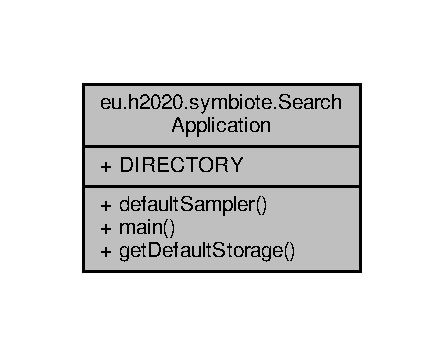
\includegraphics[width=213pt]{classeu_1_1h2020_1_1symbiote_1_1SearchApplication__coll__graph}
\end{center}
\end{figure}
\subsection*{Classes}
\begin{DoxyCompactItemize}
\item 
class {\bfseries C\+LR}
\item 
class {\bfseries Registration\+Controller}
\end{DoxyCompactItemize}
\subsection*{Public Member Functions}
\begin{DoxyCompactItemize}
\item 
Always\+Sampler {\bfseries default\+Sampler} ()\hypertarget{classeu_1_1h2020_1_1symbiote_1_1SearchApplication_a789d12cf4a0d122b6c98c80c096df80f}{}\label{classeu_1_1h2020_1_1symbiote_1_1SearchApplication_a789d12cf4a0d122b6c98c80c096df80f}

\end{DoxyCompactItemize}
\subsection*{Static Public Member Functions}
\begin{DoxyCompactItemize}
\item 
static void {\bfseries main} (String\mbox{[}$\,$\mbox{]} args)\hypertarget{classeu_1_1h2020_1_1symbiote_1_1SearchApplication_a2b0c8c4af325bf537ced8a3dd570f5eb}{}\label{classeu_1_1h2020_1_1symbiote_1_1SearchApplication_a2b0c8c4af325bf537ced8a3dd570f5eb}

\item 
static \hyperlink{classeu_1_1h2020_1_1symbiote_1_1search_1_1SearchStorage}{Search\+Storage} {\bfseries get\+Default\+Storage} ()\hypertarget{classeu_1_1h2020_1_1symbiote_1_1SearchApplication_a05ab1920a276d64229ad90d68471b34d}{}\label{classeu_1_1h2020_1_1symbiote_1_1SearchApplication_a05ab1920a276d64229ad90d68471b34d}

\end{DoxyCompactItemize}
\subsection*{Static Public Attributes}
\begin{DoxyCompactItemize}
\item 
static final String {\bfseries D\+I\+R\+E\+C\+T\+O\+RY} = System.\+get\+Property(\char`\"{}user.\+home\char`\"{}) +File.\+separator+ \char`\"{}core\+Search\+Triplestore\char`\"{}\hypertarget{classeu_1_1h2020_1_1symbiote_1_1SearchApplication_a743c407e2c7e2db78f96205fada200e7}{}\label{classeu_1_1h2020_1_1symbiote_1_1SearchApplication_a743c407e2c7e2db78f96205fada200e7}

\end{DoxyCompactItemize}


\subsection{Detailed Description}
Created by mateuszl on 22.\+09.\+2016. 

The documentation for this class was generated from the following file\+:\begin{DoxyCompactItemize}
\item 
src/main/java/eu/h2020/symbiote/Search\+Application.\+java\end{DoxyCompactItemize}

\hypertarget{classeu_1_1h2020_1_1symbiote_1_1ontology_1_1model_1_1SearchEngine}{}\section{eu.\+h2020.\+symbiote.\+ontology.\+model.\+Search\+Engine Class Reference}
\label{classeu_1_1h2020_1_1symbiote_1_1ontology_1_1model_1_1SearchEngine}\index{eu.\+h2020.\+symbiote.\+ontology.\+model.\+Search\+Engine@{eu.\+h2020.\+symbiote.\+ontology.\+model.\+Search\+Engine}}


Collaboration diagram for eu.\+h2020.\+symbiote.\+ontology.\+model.\+Search\+Engine\+:
\nopagebreak
\begin{figure}[H]
\begin{center}
\leavevmode
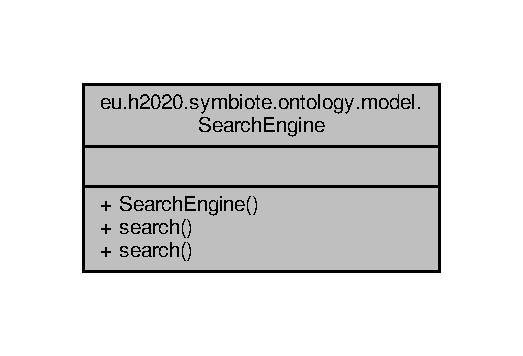
\includegraphics[width=251pt]{classeu_1_1h2020_1_1symbiote_1_1ontology_1_1model_1_1SearchEngine__coll__graph}
\end{center}
\end{figure}
\subsection*{Public Member Functions}
\begin{DoxyCompactItemize}
\item 
{\bfseries Search\+Engine} (\hyperlink{classeu_1_1h2020_1_1symbiote_1_1ontology_1_1model_1_1TripleStore}{Triple\+Store} triple\+Store)\hypertarget{classeu_1_1h2020_1_1symbiote_1_1ontology_1_1model_1_1SearchEngine_a2327a125eb5fdbe1e6ef334a3e67f04b}{}\label{classeu_1_1h2020_1_1symbiote_1_1ontology_1_1model_1_1SearchEngine_a2327a125eb5fdbe1e6ef334a3e67f04b}

\item 
Result\+Set {\bfseries search} (String model\+Graph\+Uri, String query)\hypertarget{classeu_1_1h2020_1_1symbiote_1_1ontology_1_1model_1_1SearchEngine_ac5e5ea7afb2d572c1eff6e480ace3b45}{}\label{classeu_1_1h2020_1_1symbiote_1_1ontology_1_1model_1_1SearchEngine_ac5e5ea7afb2d572c1eff6e480ace3b45}

\item 
Result\+Set {\bfseries search} (Query query)\hypertarget{classeu_1_1h2020_1_1symbiote_1_1ontology_1_1model_1_1SearchEngine_ab99e37e222402f39a899f696e40c962d}{}\label{classeu_1_1h2020_1_1symbiote_1_1ontology_1_1model_1_1SearchEngine_ab99e37e222402f39a899f696e40c962d}

\end{DoxyCompactItemize}


\subsection{Detailed Description}
\begin{DoxyAuthor}{Author}
jab 
\end{DoxyAuthor}


The documentation for this class was generated from the following file\+:\begin{DoxyCompactItemize}
\item 
src/main/java/eu/h2020/symbiote/ontology/model/Search\+Engine.\+java\end{DoxyCompactItemize}

\hypertarget{classeu_1_1h2020_1_1symbiote_1_1handlers_1_1SearchHandler}{}\section{eu.\+h2020.\+symbiote.\+handlers.\+Search\+Handler Class Reference}
\label{classeu_1_1h2020_1_1symbiote_1_1handlers_1_1SearchHandler}\index{eu.\+h2020.\+symbiote.\+handlers.\+Search\+Handler@{eu.\+h2020.\+symbiote.\+handlers.\+Search\+Handler}}


Inheritance diagram for eu.\+h2020.\+symbiote.\+handlers.\+Search\+Handler\+:
\nopagebreak
\begin{figure}[H]
\begin{center}
\leavevmode
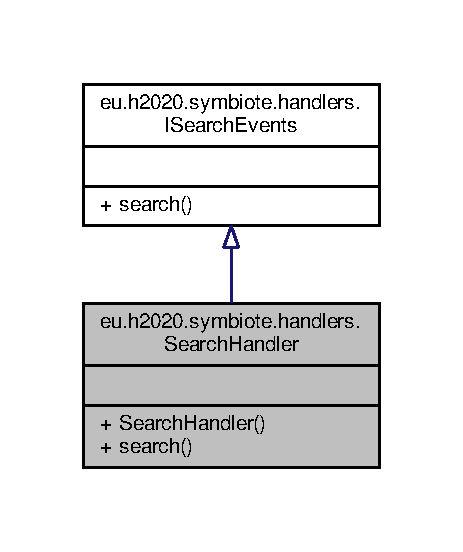
\includegraphics[width=222pt]{classeu_1_1h2020_1_1symbiote_1_1handlers_1_1SearchHandler__inherit__graph}
\end{center}
\end{figure}


Collaboration diagram for eu.\+h2020.\+symbiote.\+handlers.\+Search\+Handler\+:
\nopagebreak
\begin{figure}[H]
\begin{center}
\leavevmode
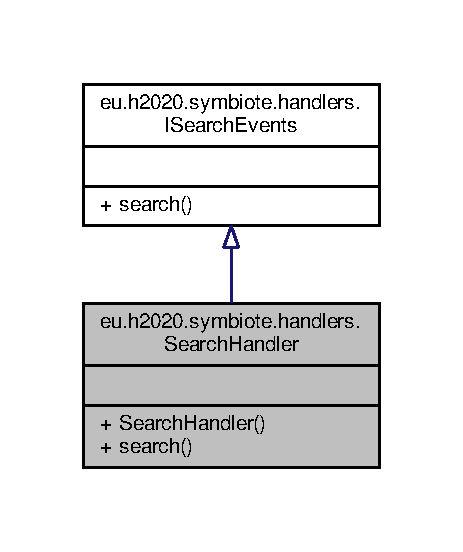
\includegraphics[width=222pt]{classeu_1_1h2020_1_1symbiote_1_1handlers_1_1SearchHandler__coll__graph}
\end{center}
\end{figure}
\subsection*{Public Member Functions}
\begin{DoxyCompactItemize}
\item 
\hyperlink{classeu_1_1h2020_1_1symbiote_1_1handlers_1_1SearchHandler_a905e2231d87dbd13de2a1d10932438b1}{Search\+Handler} (\hyperlink{classeu_1_1h2020_1_1symbiote_1_1ontology_1_1model_1_1TripleStore}{Triple\+Store} triplestore)
\item 
\hyperlink{classeu_1_1h2020_1_1symbiote_1_1query_1_1SearchResponse}{Search\+Response} \hyperlink{classeu_1_1h2020_1_1symbiote_1_1handlers_1_1SearchHandler_aa1657bbaf89181f753c550f70606ec4c}{search} (\hyperlink{classeu_1_1h2020_1_1symbiote_1_1query_1_1SearchRequest}{Search\+Request} request)
\end{DoxyCompactItemize}


\subsection{Detailed Description}
Implementation of the handler for the platform related events.

Created by Mael on 11/01/2017. 

\subsection{Constructor \& Destructor Documentation}
\index{eu\+::h2020\+::symbiote\+::handlers\+::\+Search\+Handler@{eu\+::h2020\+::symbiote\+::handlers\+::\+Search\+Handler}!Search\+Handler@{Search\+Handler}}
\index{Search\+Handler@{Search\+Handler}!eu\+::h2020\+::symbiote\+::handlers\+::\+Search\+Handler@{eu\+::h2020\+::symbiote\+::handlers\+::\+Search\+Handler}}
\subsubsection[{\texorpdfstring{Search\+Handler(\+Triple\+Store triplestore)}{SearchHandler(TripleStore triplestore)}}]{\setlength{\rightskip}{0pt plus 5cm}eu.\+h2020.\+symbiote.\+handlers.\+Search\+Handler.\+Search\+Handler (
\begin{DoxyParamCaption}
\item[{{\bf Triple\+Store}}]{triplestore}
\end{DoxyParamCaption}
)}\hypertarget{classeu_1_1h2020_1_1symbiote_1_1handlers_1_1SearchHandler_a905e2231d87dbd13de2a1d10932438b1}{}\label{classeu_1_1h2020_1_1symbiote_1_1handlers_1_1SearchHandler_a905e2231d87dbd13de2a1d10932438b1}
Create a handler of the platform events for specified storage.


\begin{DoxyParams}{Parameters}
{\em triplestore} & Triplestore on which the events should be executed. \\
\hline
\end{DoxyParams}


\subsection{Member Function Documentation}
\index{eu\+::h2020\+::symbiote\+::handlers\+::\+Search\+Handler@{eu\+::h2020\+::symbiote\+::handlers\+::\+Search\+Handler}!search@{search}}
\index{search@{search}!eu\+::h2020\+::symbiote\+::handlers\+::\+Search\+Handler@{eu\+::h2020\+::symbiote\+::handlers\+::\+Search\+Handler}}
\subsubsection[{\texorpdfstring{search(\+Search\+Request request)}{search(SearchRequest request)}}]{\setlength{\rightskip}{0pt plus 5cm}{\bf Search\+Response} eu.\+h2020.\+symbiote.\+handlers.\+Search\+Handler.\+search (
\begin{DoxyParamCaption}
\item[{{\bf Search\+Request}}]{request}
\end{DoxyParamCaption}
)}\hypertarget{classeu_1_1h2020_1_1symbiote_1_1handlers_1_1SearchHandler_aa1657bbaf89181f753c550f70606ec4c}{}\label{classeu_1_1h2020_1_1symbiote_1_1handlers_1_1SearchHandler_aa1657bbaf89181f753c550f70606ec4c}
Performs search in the module.


\begin{DoxyParams}{Parameters}
{\em request} & Request containing parameters of the search \\
\hline
\end{DoxyParams}
\begin{DoxyReturn}{Returns}
Response containing list of found resources. 
\end{DoxyReturn}


Implements \hyperlink{interfaceeu_1_1h2020_1_1symbiote_1_1handlers_1_1ISearchEvents_abbd01c728a329c40370c76d7eea20b12}{eu.\+h2020.\+symbiote.\+handlers.\+I\+Search\+Events}.



The documentation for this class was generated from the following file\+:\begin{DoxyCompactItemize}
\item 
src/main/java/eu/h2020/symbiote/handlers/Search\+Handler.\+java\end{DoxyCompactItemize}

\hypertarget{classeu_1_1h2020_1_1symbiote_1_1query_1_1SearchRequest}{}\section{eu.\+h2020.\+symbiote.\+query.\+Search\+Request Class Reference}
\label{classeu_1_1h2020_1_1symbiote_1_1query_1_1SearchRequest}\index{eu.\+h2020.\+symbiote.\+query.\+Search\+Request@{eu.\+h2020.\+symbiote.\+query.\+Search\+Request}}


Collaboration diagram for eu.\+h2020.\+symbiote.\+query.\+Search\+Request\+:
\nopagebreak
\begin{figure}[H]
\begin{center}
\leavevmode
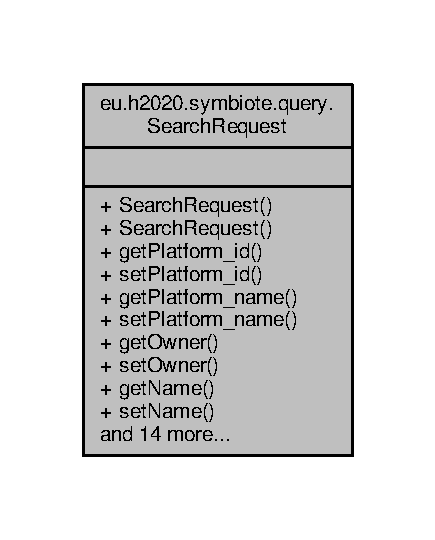
\includegraphics[width=209pt]{classeu_1_1h2020_1_1symbiote_1_1query_1_1SearchRequest__coll__graph}
\end{center}
\end{figure}
\subsection*{Public Member Functions}
\begin{DoxyCompactItemize}
\item 
{\bfseries Search\+Request} (String platform\+\_\+id, String platform\+\_\+name, String owner, String name, String id, String description, String location\+\_\+name, Double location\+\_\+lat, Double location\+\_\+long, Integer max\+\_\+distance, List$<$ String $>$ observed\+\_\+property)\hypertarget{classeu_1_1h2020_1_1symbiote_1_1query_1_1SearchRequest_a3542fa8f475209e293d35ce5a6d3922f}{}\label{classeu_1_1h2020_1_1symbiote_1_1query_1_1SearchRequest_a3542fa8f475209e293d35ce5a6d3922f}

\item 
String {\bfseries get\+Platform\+\_\+id} ()\hypertarget{classeu_1_1h2020_1_1symbiote_1_1query_1_1SearchRequest_ae4a375a18e472d125ae59c6d21ce2706}{}\label{classeu_1_1h2020_1_1symbiote_1_1query_1_1SearchRequest_ae4a375a18e472d125ae59c6d21ce2706}

\item 
void {\bfseries set\+Platform\+\_\+id} (String platform\+\_\+id)\hypertarget{classeu_1_1h2020_1_1symbiote_1_1query_1_1SearchRequest_a2dad4ea31087b03d9362c459b818f529}{}\label{classeu_1_1h2020_1_1symbiote_1_1query_1_1SearchRequest_a2dad4ea31087b03d9362c459b818f529}

\item 
String {\bfseries get\+Platform\+\_\+name} ()\hypertarget{classeu_1_1h2020_1_1symbiote_1_1query_1_1SearchRequest_a2802002b4a55158842805611dfda58e8}{}\label{classeu_1_1h2020_1_1symbiote_1_1query_1_1SearchRequest_a2802002b4a55158842805611dfda58e8}

\item 
void {\bfseries set\+Platform\+\_\+name} (String platform\+\_\+name)\hypertarget{classeu_1_1h2020_1_1symbiote_1_1query_1_1SearchRequest_aae4453d7d3ae14888e773647a153c839}{}\label{classeu_1_1h2020_1_1symbiote_1_1query_1_1SearchRequest_aae4453d7d3ae14888e773647a153c839}

\item 
String {\bfseries get\+Owner} ()\hypertarget{classeu_1_1h2020_1_1symbiote_1_1query_1_1SearchRequest_a734f9cfa7013a2359a6cee120da22360}{}\label{classeu_1_1h2020_1_1symbiote_1_1query_1_1SearchRequest_a734f9cfa7013a2359a6cee120da22360}

\item 
void {\bfseries set\+Owner} (String owner)\hypertarget{classeu_1_1h2020_1_1symbiote_1_1query_1_1SearchRequest_acca5d0888282dce7c86f835439f7ac91}{}\label{classeu_1_1h2020_1_1symbiote_1_1query_1_1SearchRequest_acca5d0888282dce7c86f835439f7ac91}

\item 
String {\bfseries get\+Name} ()\hypertarget{classeu_1_1h2020_1_1symbiote_1_1query_1_1SearchRequest_a6a9651ad510ef2e1be05fc90082faa86}{}\label{classeu_1_1h2020_1_1symbiote_1_1query_1_1SearchRequest_a6a9651ad510ef2e1be05fc90082faa86}

\item 
void {\bfseries set\+Name} (String name)\hypertarget{classeu_1_1h2020_1_1symbiote_1_1query_1_1SearchRequest_ade7afb719ef519a0b8e559811c5931e2}{}\label{classeu_1_1h2020_1_1symbiote_1_1query_1_1SearchRequest_ade7afb719ef519a0b8e559811c5931e2}

\item 
String {\bfseries get\+Id} ()\hypertarget{classeu_1_1h2020_1_1symbiote_1_1query_1_1SearchRequest_a6753de2db3ff6b005ea43f6d140e01dc}{}\label{classeu_1_1h2020_1_1symbiote_1_1query_1_1SearchRequest_a6753de2db3ff6b005ea43f6d140e01dc}

\item 
void {\bfseries set\+Id} (String id)\hypertarget{classeu_1_1h2020_1_1symbiote_1_1query_1_1SearchRequest_ade59c68f7c756da7ae511c480525746d}{}\label{classeu_1_1h2020_1_1symbiote_1_1query_1_1SearchRequest_ade59c68f7c756da7ae511c480525746d}

\item 
String {\bfseries get\+Description} ()\hypertarget{classeu_1_1h2020_1_1symbiote_1_1query_1_1SearchRequest_ae0ff9e2f29badf203e358f16709927c6}{}\label{classeu_1_1h2020_1_1symbiote_1_1query_1_1SearchRequest_ae0ff9e2f29badf203e358f16709927c6}

\item 
void {\bfseries set\+Description} (String description)\hypertarget{classeu_1_1h2020_1_1symbiote_1_1query_1_1SearchRequest_a0c2f3e011dd94d01fb9a868b1fdafd13}{}\label{classeu_1_1h2020_1_1symbiote_1_1query_1_1SearchRequest_a0c2f3e011dd94d01fb9a868b1fdafd13}

\item 
String {\bfseries get\+Location\+\_\+name} ()\hypertarget{classeu_1_1h2020_1_1symbiote_1_1query_1_1SearchRequest_a832611dd1f4a9de035825f207dac4de8}{}\label{classeu_1_1h2020_1_1symbiote_1_1query_1_1SearchRequest_a832611dd1f4a9de035825f207dac4de8}

\item 
void {\bfseries set\+Location\+\_\+name} (String location\+\_\+name)\hypertarget{classeu_1_1h2020_1_1symbiote_1_1query_1_1SearchRequest_a0792e2bb5bf5dfa78e1e3cd2a9fb5efb}{}\label{classeu_1_1h2020_1_1symbiote_1_1query_1_1SearchRequest_a0792e2bb5bf5dfa78e1e3cd2a9fb5efb}

\item 
Double {\bfseries get\+Location\+\_\+lat} ()\hypertarget{classeu_1_1h2020_1_1symbiote_1_1query_1_1SearchRequest_afc417e6e5d426d1862e3e9e1311314c6}{}\label{classeu_1_1h2020_1_1symbiote_1_1query_1_1SearchRequest_afc417e6e5d426d1862e3e9e1311314c6}

\item 
void {\bfseries set\+Location\+\_\+lat} (Double location\+\_\+lat)\hypertarget{classeu_1_1h2020_1_1symbiote_1_1query_1_1SearchRequest_a64aa50edc04e5ef88d65d9b8dfc59828}{}\label{classeu_1_1h2020_1_1symbiote_1_1query_1_1SearchRequest_a64aa50edc04e5ef88d65d9b8dfc59828}

\item 
Double {\bfseries get\+Location\+\_\+long} ()\hypertarget{classeu_1_1h2020_1_1symbiote_1_1query_1_1SearchRequest_a30dc9dca9e7053cc705cf80c39b8d6b3}{}\label{classeu_1_1h2020_1_1symbiote_1_1query_1_1SearchRequest_a30dc9dca9e7053cc705cf80c39b8d6b3}

\item 
void {\bfseries set\+Location\+\_\+long} (Double location\+\_\+long)\hypertarget{classeu_1_1h2020_1_1symbiote_1_1query_1_1SearchRequest_af377b74d02c4ee433e13f0c2a50eae1b}{}\label{classeu_1_1h2020_1_1symbiote_1_1query_1_1SearchRequest_af377b74d02c4ee433e13f0c2a50eae1b}

\item 
Integer {\bfseries get\+Max\+\_\+distance} ()\hypertarget{classeu_1_1h2020_1_1symbiote_1_1query_1_1SearchRequest_abe26768baed48be4cbde5bfd8b4c7a0d}{}\label{classeu_1_1h2020_1_1symbiote_1_1query_1_1SearchRequest_abe26768baed48be4cbde5bfd8b4c7a0d}

\item 
void {\bfseries set\+Max\+\_\+distance} (Integer max\+\_\+distance)\hypertarget{classeu_1_1h2020_1_1symbiote_1_1query_1_1SearchRequest_af3b45851073a2bdbffdbe4bb1fc478d9}{}\label{classeu_1_1h2020_1_1symbiote_1_1query_1_1SearchRequest_af3b45851073a2bdbffdbe4bb1fc478d9}

\item 
List$<$ String $>$ {\bfseries get\+Observed\+\_\+property} ()\hypertarget{classeu_1_1h2020_1_1symbiote_1_1query_1_1SearchRequest_af9050259cfb63e802cd654c2e8d7e538}{}\label{classeu_1_1h2020_1_1symbiote_1_1query_1_1SearchRequest_af9050259cfb63e802cd654c2e8d7e538}

\item 
void {\bfseries set\+Observed\+\_\+property} (List$<$ String $>$ observed\+\_\+property)\hypertarget{classeu_1_1h2020_1_1symbiote_1_1query_1_1SearchRequest_a16e9d33081fd64243d67e4f97ec6300e}{}\label{classeu_1_1h2020_1_1symbiote_1_1query_1_1SearchRequest_a16e9d33081fd64243d67e4f97ec6300e}

\end{DoxyCompactItemize}


\subsection{Detailed Description}
Class representing search query request.

Created by Mael on 24/01/2017. 

The documentation for this class was generated from the following file\+:\begin{DoxyCompactItemize}
\item 
src/main/java/eu/h2020/symbiote/query/Search\+Request.\+java\end{DoxyCompactItemize}

\hypertarget{classeu_1_1h2020_1_1symbiote_1_1communication_1_1SearchRequestedConsumer}{}\section{eu.\+h2020.\+symbiote.\+communication.\+Search\+Requested\+Consumer Class Reference}
\label{classeu_1_1h2020_1_1symbiote_1_1communication_1_1SearchRequestedConsumer}\index{eu.\+h2020.\+symbiote.\+communication.\+Search\+Requested\+Consumer@{eu.\+h2020.\+symbiote.\+communication.\+Search\+Requested\+Consumer}}


Inheritance diagram for eu.\+h2020.\+symbiote.\+communication.\+Search\+Requested\+Consumer\+:
\nopagebreak
\begin{figure}[H]
\begin{center}
\leavevmode
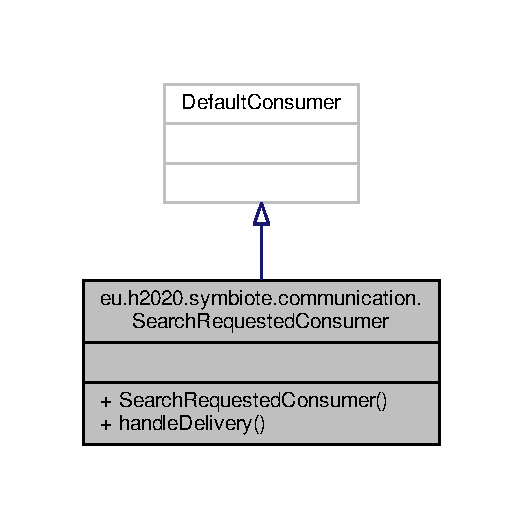
\includegraphics[width=251pt]{classeu_1_1h2020_1_1symbiote_1_1communication_1_1SearchRequestedConsumer__inherit__graph}
\end{center}
\end{figure}


Collaboration diagram for eu.\+h2020.\+symbiote.\+communication.\+Search\+Requested\+Consumer\+:
\nopagebreak
\begin{figure}[H]
\begin{center}
\leavevmode
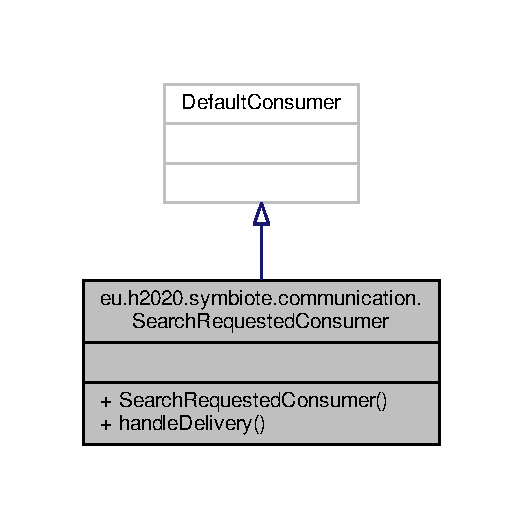
\includegraphics[width=251pt]{classeu_1_1h2020_1_1symbiote_1_1communication_1_1SearchRequestedConsumer__coll__graph}
\end{center}
\end{figure}
\subsection*{Public Member Functions}
\begin{DoxyCompactItemize}
\item 
\hyperlink{classeu_1_1h2020_1_1symbiote_1_1communication_1_1SearchRequestedConsumer_ab7f2928dacf9df2f63cf8c94daa87442}{Search\+Requested\+Consumer} (Channel channel, \hyperlink{classeu_1_1h2020_1_1symbiote_1_1handlers_1_1SearchHandler}{Search\+Handler} handler)
\item 
void {\bfseries handle\+Delivery} (String consumer\+Tag, Envelope envelope, A\+M\+Q\+P.\+Basic\+Properties properties, byte\mbox{[}$\,$\mbox{]} body)  throws I\+O\+Exception \hypertarget{classeu_1_1h2020_1_1symbiote_1_1communication_1_1SearchRequestedConsumer_a473b8ac445d9ee29b81727c845f6e7ab}{}\label{classeu_1_1h2020_1_1symbiote_1_1communication_1_1SearchRequestedConsumer_a473b8ac445d9ee29b81727c845f6e7ab}

\end{DoxyCompactItemize}


\subsection{Detailed Description}
Consumer of the search requested event. Translates the message as list of query parameters, translates them into S\+P\+A\+R\+QL and queries the repository.

Created by Mael on 17/01/2017. 

\subsection{Constructor \& Destructor Documentation}
\index{eu\+::h2020\+::symbiote\+::communication\+::\+Search\+Requested\+Consumer@{eu\+::h2020\+::symbiote\+::communication\+::\+Search\+Requested\+Consumer}!Search\+Requested\+Consumer@{Search\+Requested\+Consumer}}
\index{Search\+Requested\+Consumer@{Search\+Requested\+Consumer}!eu\+::h2020\+::symbiote\+::communication\+::\+Search\+Requested\+Consumer@{eu\+::h2020\+::symbiote\+::communication\+::\+Search\+Requested\+Consumer}}
\subsubsection[{\texorpdfstring{Search\+Requested\+Consumer(\+Channel channel, Search\+Handler handler)}{SearchRequestedConsumer(Channel channel, SearchHandler handler)}}]{\setlength{\rightskip}{0pt plus 5cm}eu.\+h2020.\+symbiote.\+communication.\+Search\+Requested\+Consumer.\+Search\+Requested\+Consumer (
\begin{DoxyParamCaption}
\item[{Channel}]{channel, }
\item[{{\bf Search\+Handler}}]{handler}
\end{DoxyParamCaption}
)}\hypertarget{classeu_1_1h2020_1_1symbiote_1_1communication_1_1SearchRequestedConsumer_ab7f2928dacf9df2f63cf8c94daa87442}{}\label{classeu_1_1h2020_1_1symbiote_1_1communication_1_1SearchRequestedConsumer_ab7f2928dacf9df2f63cf8c94daa87442}
Constructs a new instance and records its association to the passed-\/in channel.


\begin{DoxyParams}{Parameters}
{\em channel} & the channel to which this consumer is attached \\
\hline
{\em handler} & handler to be used by the consumer. \\
\hline
\end{DoxyParams}


The documentation for this class was generated from the following file\+:\begin{DoxyCompactItemize}
\item 
src/main/java/eu/h2020/symbiote/communication/Search\+Requested\+Consumer.\+java\end{DoxyCompactItemize}

\hypertarget{classeu_1_1h2020_1_1symbiote_1_1query_1_1SearchResponse}{}\section{eu.\+h2020.\+symbiote.\+query.\+Search\+Response Class Reference}
\label{classeu_1_1h2020_1_1symbiote_1_1query_1_1SearchResponse}\index{eu.\+h2020.\+symbiote.\+query.\+Search\+Response@{eu.\+h2020.\+symbiote.\+query.\+Search\+Response}}


Collaboration diagram for eu.\+h2020.\+symbiote.\+query.\+Search\+Response\+:
\nopagebreak
\begin{figure}[H]
\begin{center}
\leavevmode
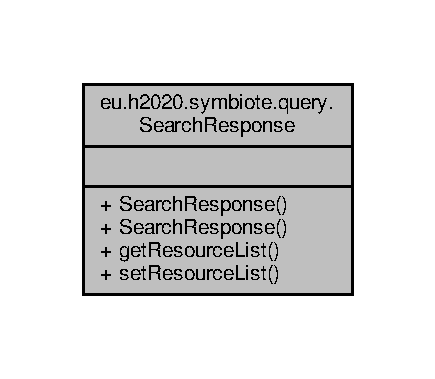
\includegraphics[width=209pt]{classeu_1_1h2020_1_1symbiote_1_1query_1_1SearchResponse__coll__graph}
\end{center}
\end{figure}
\subsection*{Public Member Functions}
\begin{DoxyCompactItemize}
\item 
{\bfseries Search\+Response} (List$<$ \hyperlink{classeu_1_1h2020_1_1symbiote_1_1query_1_1SearchResponseResource}{Search\+Response\+Resource} $>$ resource\+List)\hypertarget{classeu_1_1h2020_1_1symbiote_1_1query_1_1SearchResponse_a9138f72bc4db26c6bd99e9f9a1056178}{}\label{classeu_1_1h2020_1_1symbiote_1_1query_1_1SearchResponse_a9138f72bc4db26c6bd99e9f9a1056178}

\item 
List$<$ \hyperlink{classeu_1_1h2020_1_1symbiote_1_1query_1_1SearchResponseResource}{Search\+Response\+Resource} $>$ {\bfseries get\+Resource\+List} ()\hypertarget{classeu_1_1h2020_1_1symbiote_1_1query_1_1SearchResponse_ab07365c07e7f809df1f9f5133ddd7a11}{}\label{classeu_1_1h2020_1_1symbiote_1_1query_1_1SearchResponse_ab07365c07e7f809df1f9f5133ddd7a11}

\item 
void {\bfseries set\+Resource\+List} (List$<$ \hyperlink{classeu_1_1h2020_1_1symbiote_1_1query_1_1SearchResponseResource}{Search\+Response\+Resource} $>$ resource\+List)\hypertarget{classeu_1_1h2020_1_1symbiote_1_1query_1_1SearchResponse_af12485f7910ec0f088ef8d45d2c524aa}{}\label{classeu_1_1h2020_1_1symbiote_1_1query_1_1SearchResponse_af12485f7910ec0f088ef8d45d2c524aa}

\end{DoxyCompactItemize}


\subsection{Detailed Description}
A response to the query containing a list of resources fulfilling the requirements.

Created by Mael on 24/01/2017. 

The documentation for this class was generated from the following file\+:\begin{DoxyCompactItemize}
\item 
src/main/java/eu/h2020/symbiote/query/Search\+Response.\+java\end{DoxyCompactItemize}

\hypertarget{classeu_1_1h2020_1_1symbiote_1_1query_1_1SearchResponseResource}{}\section{eu.\+h2020.\+symbiote.\+query.\+Search\+Response\+Resource Class Reference}
\label{classeu_1_1h2020_1_1symbiote_1_1query_1_1SearchResponseResource}\index{eu.\+h2020.\+symbiote.\+query.\+Search\+Response\+Resource@{eu.\+h2020.\+symbiote.\+query.\+Search\+Response\+Resource}}


Collaboration diagram for eu.\+h2020.\+symbiote.\+query.\+Search\+Response\+Resource\+:
\nopagebreak
\begin{figure}[H]
\begin{center}
\leavevmode
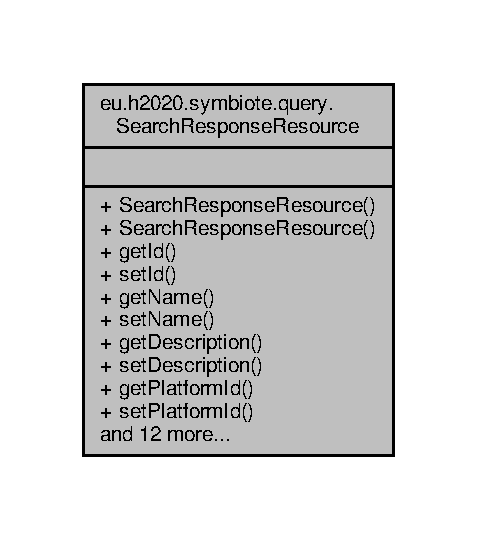
\includegraphics[width=229pt]{classeu_1_1h2020_1_1symbiote_1_1query_1_1SearchResponseResource__coll__graph}
\end{center}
\end{figure}
\subsection*{Public Member Functions}
\begin{DoxyCompactItemize}
\item 
{\bfseries Search\+Response\+Resource} (String id, String name, String description, String platform\+Id, String platform\+Name, String location\+Name, Double location\+Latitude, Double location\+Longitude, Double location\+Altitude, List$<$ String $>$ observed\+Properties)\hypertarget{classeu_1_1h2020_1_1symbiote_1_1query_1_1SearchResponseResource_a2cea8e2054c2d25a53c13153293c33d3}{}\label{classeu_1_1h2020_1_1symbiote_1_1query_1_1SearchResponseResource_a2cea8e2054c2d25a53c13153293c33d3}

\item 
String {\bfseries get\+Id} ()\hypertarget{classeu_1_1h2020_1_1symbiote_1_1query_1_1SearchResponseResource_adeb1a735b00bd99d3cf63bfa036ed851}{}\label{classeu_1_1h2020_1_1symbiote_1_1query_1_1SearchResponseResource_adeb1a735b00bd99d3cf63bfa036ed851}

\item 
void {\bfseries set\+Id} (String id)\hypertarget{classeu_1_1h2020_1_1symbiote_1_1query_1_1SearchResponseResource_af35030bd4c6033f4d05846b938a82b4b}{}\label{classeu_1_1h2020_1_1symbiote_1_1query_1_1SearchResponseResource_af35030bd4c6033f4d05846b938a82b4b}

\item 
String {\bfseries get\+Name} ()\hypertarget{classeu_1_1h2020_1_1symbiote_1_1query_1_1SearchResponseResource_a4d31fc065b27d8c018af7932167c2e96}{}\label{classeu_1_1h2020_1_1symbiote_1_1query_1_1SearchResponseResource_a4d31fc065b27d8c018af7932167c2e96}

\item 
void {\bfseries set\+Name} (String name)\hypertarget{classeu_1_1h2020_1_1symbiote_1_1query_1_1SearchResponseResource_a3870b790e9ec8a07dfb6e39ba609877b}{}\label{classeu_1_1h2020_1_1symbiote_1_1query_1_1SearchResponseResource_a3870b790e9ec8a07dfb6e39ba609877b}

\item 
String {\bfseries get\+Description} ()\hypertarget{classeu_1_1h2020_1_1symbiote_1_1query_1_1SearchResponseResource_a9a816ae05b21202629e9ee4101bae66c}{}\label{classeu_1_1h2020_1_1symbiote_1_1query_1_1SearchResponseResource_a9a816ae05b21202629e9ee4101bae66c}

\item 
void {\bfseries set\+Description} (String description)\hypertarget{classeu_1_1h2020_1_1symbiote_1_1query_1_1SearchResponseResource_a8e8e92d882aa8d6ec21092c88ab0f2e9}{}\label{classeu_1_1h2020_1_1symbiote_1_1query_1_1SearchResponseResource_a8e8e92d882aa8d6ec21092c88ab0f2e9}

\item 
String {\bfseries get\+Platform\+Id} ()\hypertarget{classeu_1_1h2020_1_1symbiote_1_1query_1_1SearchResponseResource_af1f966b845ff1d3d47f9abac2b1d1de1}{}\label{classeu_1_1h2020_1_1symbiote_1_1query_1_1SearchResponseResource_af1f966b845ff1d3d47f9abac2b1d1de1}

\item 
void {\bfseries set\+Platform\+Id} (String platform\+Id)\hypertarget{classeu_1_1h2020_1_1symbiote_1_1query_1_1SearchResponseResource_a703fa99219c7946cee4c5208332952cc}{}\label{classeu_1_1h2020_1_1symbiote_1_1query_1_1SearchResponseResource_a703fa99219c7946cee4c5208332952cc}

\item 
String {\bfseries get\+Platform\+Name} ()\hypertarget{classeu_1_1h2020_1_1symbiote_1_1query_1_1SearchResponseResource_ae7d93111be388d02896a74683ffe8d7c}{}\label{classeu_1_1h2020_1_1symbiote_1_1query_1_1SearchResponseResource_ae7d93111be388d02896a74683ffe8d7c}

\item 
void {\bfseries set\+Platform\+Name} (String platform\+Name)\hypertarget{classeu_1_1h2020_1_1symbiote_1_1query_1_1SearchResponseResource_a03fda1de8b29ffe817495e05d56eb2d3}{}\label{classeu_1_1h2020_1_1symbiote_1_1query_1_1SearchResponseResource_a03fda1de8b29ffe817495e05d56eb2d3}

\item 
String {\bfseries get\+Location\+Name} ()\hypertarget{classeu_1_1h2020_1_1symbiote_1_1query_1_1SearchResponseResource_ab3d504d0e2ba85165579bda7fe92f449}{}\label{classeu_1_1h2020_1_1symbiote_1_1query_1_1SearchResponseResource_ab3d504d0e2ba85165579bda7fe92f449}

\item 
void {\bfseries set\+Location\+Name} (String location\+Name)\hypertarget{classeu_1_1h2020_1_1symbiote_1_1query_1_1SearchResponseResource_a03fbeec61ad4e5b4340a1a32c3c068a9}{}\label{classeu_1_1h2020_1_1symbiote_1_1query_1_1SearchResponseResource_a03fbeec61ad4e5b4340a1a32c3c068a9}

\item 
Double {\bfseries get\+Location\+Latitude} ()\hypertarget{classeu_1_1h2020_1_1symbiote_1_1query_1_1SearchResponseResource_a717e2308de157056a47ac7106f842c11}{}\label{classeu_1_1h2020_1_1symbiote_1_1query_1_1SearchResponseResource_a717e2308de157056a47ac7106f842c11}

\item 
void {\bfseries set\+Location\+Latitude} (Double location\+Latitude)\hypertarget{classeu_1_1h2020_1_1symbiote_1_1query_1_1SearchResponseResource_a43da6fb510f261208f90e4efe8793d3d}{}\label{classeu_1_1h2020_1_1symbiote_1_1query_1_1SearchResponseResource_a43da6fb510f261208f90e4efe8793d3d}

\item 
Double {\bfseries get\+Location\+Longitude} ()\hypertarget{classeu_1_1h2020_1_1symbiote_1_1query_1_1SearchResponseResource_a6dc65e2054edde99e488199b21c2dbea}{}\label{classeu_1_1h2020_1_1symbiote_1_1query_1_1SearchResponseResource_a6dc65e2054edde99e488199b21c2dbea}

\item 
void {\bfseries set\+Location\+Longitude} (Double location\+Longitude)\hypertarget{classeu_1_1h2020_1_1symbiote_1_1query_1_1SearchResponseResource_ae5b89a286f54a9118916ede8e23180b7}{}\label{classeu_1_1h2020_1_1symbiote_1_1query_1_1SearchResponseResource_ae5b89a286f54a9118916ede8e23180b7}

\item 
Double {\bfseries get\+Location\+Altitude} ()\hypertarget{classeu_1_1h2020_1_1symbiote_1_1query_1_1SearchResponseResource_af63e588b34554c25eaaa0e0299972bf2}{}\label{classeu_1_1h2020_1_1symbiote_1_1query_1_1SearchResponseResource_af63e588b34554c25eaaa0e0299972bf2}

\item 
void {\bfseries set\+Location\+Altitude} (Double location\+Altitude)\hypertarget{classeu_1_1h2020_1_1symbiote_1_1query_1_1SearchResponseResource_a5ced25d930ab4e626e83c2694910eb8d}{}\label{classeu_1_1h2020_1_1symbiote_1_1query_1_1SearchResponseResource_a5ced25d930ab4e626e83c2694910eb8d}

\item 
List$<$ String $>$ {\bfseries get\+Observed\+Properties} ()\hypertarget{classeu_1_1h2020_1_1symbiote_1_1query_1_1SearchResponseResource_a324f113a00a6efe96fb0f12de75ddb72}{}\label{classeu_1_1h2020_1_1symbiote_1_1query_1_1SearchResponseResource_a324f113a00a6efe96fb0f12de75ddb72}

\item 
void {\bfseries set\+Observed\+Properties} (List$<$ String $>$ observed\+Properties)\hypertarget{classeu_1_1h2020_1_1symbiote_1_1query_1_1SearchResponseResource_a6dbd57313f4ae304085d1ed1ad6d850f}{}\label{classeu_1_1h2020_1_1symbiote_1_1query_1_1SearchResponseResource_a6dbd57313f4ae304085d1ed1ad6d850f}

\end{DoxyCompactItemize}


\subsection{Detailed Description}
Single response for a query.

Created by Mael on 24/01/2017. 

The documentation for this class was generated from the following file\+:\begin{DoxyCompactItemize}
\item 
src/main/java/eu/h2020/symbiote/query/Search\+Response\+Resource.\+java\end{DoxyCompactItemize}

\hypertarget{classeu_1_1h2020_1_1symbiote_1_1search_1_1SearchStorage}{}\section{eu.\+h2020.\+symbiote.\+search.\+Search\+Storage Class Reference}
\label{classeu_1_1h2020_1_1symbiote_1_1search_1_1SearchStorage}\index{eu.\+h2020.\+symbiote.\+search.\+Search\+Storage@{eu.\+h2020.\+symbiote.\+search.\+Search\+Storage}}


Collaboration diagram for eu.\+h2020.\+symbiote.\+search.\+Search\+Storage\+:
\nopagebreak
\begin{figure}[H]
\begin{center}
\leavevmode
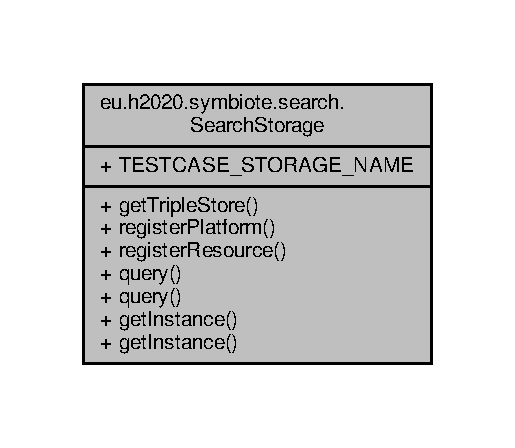
\includegraphics[width=247pt]{classeu_1_1h2020_1_1symbiote_1_1search_1_1SearchStorage__coll__graph}
\end{center}
\end{figure}
\subsection*{Public Member Functions}
\begin{DoxyCompactItemize}
\item 
\hyperlink{classeu_1_1h2020_1_1symbiote_1_1ontology_1_1model_1_1TripleStore}{Triple\+Store} \hyperlink{classeu_1_1h2020_1_1symbiote_1_1search_1_1SearchStorage_a94653338069782785b686128ea52c5c2}{get\+Triple\+Store} ()
\item 
void \hyperlink{classeu_1_1h2020_1_1symbiote_1_1search_1_1SearchStorage_a82e5bf8079db6b8ddc014e3d2cb41354}{register\+Platform} (String platform\+Id, Model rdf\+Model, String model\+Id)
\item 
void \hyperlink{classeu_1_1h2020_1_1symbiote_1_1search_1_1SearchStorage_a0b81f975b711ea0616bcfad65b9c5fdf}{register\+Resource} (String platform\+Uri, String service\+Uri, String resource\+Uri, Model rdf\+Model)
\item 
List$<$ String $>$ {\bfseries query} (String model\+Graph\+Uri, String query)\hypertarget{classeu_1_1h2020_1_1symbiote_1_1search_1_1SearchStorage_a603b3351f858aa41a36b53ee73e4eedf}{}\label{classeu_1_1h2020_1_1symbiote_1_1search_1_1SearchStorage_a603b3351f858aa41a36b53ee73e4eedf}

\item 
List$<$ String $>$ {\bfseries query} (String model\+Graph\+Uri, Query query)\hypertarget{classeu_1_1h2020_1_1symbiote_1_1search_1_1SearchStorage_a4b4426aa63015e883766359c94d64bf0}{}\label{classeu_1_1h2020_1_1symbiote_1_1search_1_1SearchStorage_a4b4426aa63015e883766359c94d64bf0}

\end{DoxyCompactItemize}
\subsection*{Static Public Member Functions}
\begin{DoxyCompactItemize}
\item 
static \hyperlink{classeu_1_1h2020_1_1symbiote_1_1search_1_1SearchStorage}{Search\+Storage} \hyperlink{classeu_1_1h2020_1_1symbiote_1_1search_1_1SearchStorage_a49404088c4dcdf94e5f0d6a85b856a5c}{get\+Instance} ()
\item 
static \hyperlink{classeu_1_1h2020_1_1symbiote_1_1search_1_1SearchStorage}{Search\+Storage} \hyperlink{classeu_1_1h2020_1_1symbiote_1_1search_1_1SearchStorage_ad8a5239e7c9df6c07b7b3bf7697f50e1}{get\+Instance} (String storage\+Name)
\end{DoxyCompactItemize}
\subsection*{Static Public Attributes}
\begin{DoxyCompactItemize}
\item 
static final String {\bfseries T\+E\+S\+T\+C\+A\+S\+E\+\_\+\+S\+T\+O\+R\+A\+G\+E\+\_\+\+N\+A\+ME} = \char`\"{}memory\+\_\+test\+\_\+storage\char`\"{}\hypertarget{classeu_1_1h2020_1_1symbiote_1_1search_1_1SearchStorage_a10c7d4c200e5f4582fcd8018e64acf06}{}\label{classeu_1_1h2020_1_1symbiote_1_1search_1_1SearchStorage_a10c7d4c200e5f4582fcd8018e64acf06}

\end{DoxyCompactItemize}


\subsection{Detailed Description}
Created by Mael on 31/08/2016. 

\subsection{Member Function Documentation}
\index{eu\+::h2020\+::symbiote\+::search\+::\+Search\+Storage@{eu\+::h2020\+::symbiote\+::search\+::\+Search\+Storage}!get\+Instance@{get\+Instance}}
\index{get\+Instance@{get\+Instance}!eu\+::h2020\+::symbiote\+::search\+::\+Search\+Storage@{eu\+::h2020\+::symbiote\+::search\+::\+Search\+Storage}}
\subsubsection[{\texorpdfstring{get\+Instance()}{getInstance()}}]{\setlength{\rightskip}{0pt plus 5cm}static {\bf Search\+Storage} eu.\+h2020.\+symbiote.\+search.\+Search\+Storage.\+get\+Instance (
\begin{DoxyParamCaption}
{}
\end{DoxyParamCaption}
)\hspace{0.3cm}{\ttfamily [static]}}\hypertarget{classeu_1_1h2020_1_1symbiote_1_1search_1_1SearchStorage_a49404088c4dcdf94e5f0d6a85b856a5c}{}\label{classeu_1_1h2020_1_1symbiote_1_1search_1_1SearchStorage_a49404088c4dcdf94e5f0d6a85b856a5c}
Gets or creates Search Storage singleton for default location

\begin{DoxyReturn}{Returns}
Singleton of the storage for default location. 
\end{DoxyReturn}
\index{eu\+::h2020\+::symbiote\+::search\+::\+Search\+Storage@{eu\+::h2020\+::symbiote\+::search\+::\+Search\+Storage}!get\+Instance@{get\+Instance}}
\index{get\+Instance@{get\+Instance}!eu\+::h2020\+::symbiote\+::search\+::\+Search\+Storage@{eu\+::h2020\+::symbiote\+::search\+::\+Search\+Storage}}
\subsubsection[{\texorpdfstring{get\+Instance(\+String storage\+Name)}{getInstance(String storageName)}}]{\setlength{\rightskip}{0pt plus 5cm}static {\bf Search\+Storage} eu.\+h2020.\+symbiote.\+search.\+Search\+Storage.\+get\+Instance (
\begin{DoxyParamCaption}
\item[{String}]{storage\+Name}
\end{DoxyParamCaption}
)\hspace{0.3cm}{\ttfamily [static]}}\hypertarget{classeu_1_1h2020_1_1symbiote_1_1search_1_1SearchStorage_ad8a5239e7c9df6c07b7b3bf7697f50e1}{}\label{classeu_1_1h2020_1_1symbiote_1_1search_1_1SearchStorage_ad8a5239e7c9df6c07b7b3bf7697f50e1}
Gets or creates Search Storage singleton for specified location.

Use T\+E\+S\+T\+C\+A\+S\+E\+\_\+\+S\+T\+O\+R\+A\+G\+E\+\_\+\+N\+A\+ME to use in-\/memory, not persistable storage (for testing/demo purpose).


\begin{DoxyParams}{Parameters}
{\em storage\+Name} & Name of the storage, which corresponds to it\textquotesingle{}s location. \\
\hline
\end{DoxyParams}
\begin{DoxyReturn}{Returns}
Singleton of the storage for location with specified name 
\end{DoxyReturn}
\index{eu\+::h2020\+::symbiote\+::search\+::\+Search\+Storage@{eu\+::h2020\+::symbiote\+::search\+::\+Search\+Storage}!get\+Triple\+Store@{get\+Triple\+Store}}
\index{get\+Triple\+Store@{get\+Triple\+Store}!eu\+::h2020\+::symbiote\+::search\+::\+Search\+Storage@{eu\+::h2020\+::symbiote\+::search\+::\+Search\+Storage}}
\subsubsection[{\texorpdfstring{get\+Triple\+Store()}{getTripleStore()}}]{\setlength{\rightskip}{0pt plus 5cm}{\bf Triple\+Store} eu.\+h2020.\+symbiote.\+search.\+Search\+Storage.\+get\+Triple\+Store (
\begin{DoxyParamCaption}
{}
\end{DoxyParamCaption}
)}\hypertarget{classeu_1_1h2020_1_1symbiote_1_1search_1_1SearchStorage_a94653338069782785b686128ea52c5c2}{}\label{classeu_1_1h2020_1_1symbiote_1_1search_1_1SearchStorage_a94653338069782785b686128ea52c5c2}
Registers ontology model in the search engine, using specified model\textquotesingle{}s id to generate model graph uri.


\begin{DoxyParams}{Parameters}
{\em model} & Model to be registered \\
\hline
\end{DoxyParams}
\index{eu\+::h2020\+::symbiote\+::search\+::\+Search\+Storage@{eu\+::h2020\+::symbiote\+::search\+::\+Search\+Storage}!register\+Platform@{register\+Platform}}
\index{register\+Platform@{register\+Platform}!eu\+::h2020\+::symbiote\+::search\+::\+Search\+Storage@{eu\+::h2020\+::symbiote\+::search\+::\+Search\+Storage}}
\subsubsection[{\texorpdfstring{register\+Platform(\+String platform\+Id, Model rdf\+Model, String model\+Id)}{registerPlatform(String platformId, Model rdfModel, String modelId)}}]{\setlength{\rightskip}{0pt plus 5cm}void eu.\+h2020.\+symbiote.\+search.\+Search\+Storage.\+register\+Platform (
\begin{DoxyParamCaption}
\item[{String}]{platform\+Id, }
\item[{Model}]{rdf\+Model, }
\item[{String}]{model\+Id}
\end{DoxyParamCaption}
)}\hypertarget{classeu_1_1h2020_1_1symbiote_1_1search_1_1SearchStorage_a82e5bf8079db6b8ddc014e3d2cb41354}{}\label{classeu_1_1h2020_1_1symbiote_1_1search_1_1SearchStorage_a82e5bf8079db6b8ddc014e3d2cb41354}
Registers platform in the search engine, using specified platform\textquotesingle{}s id to generate platform graph uri


\begin{DoxyParams}{Parameters}
{\em platform\+Id} & \\
\hline
{\em rdf\+Model} & \\
\hline
{\em model\+Id} & \\
\hline
\end{DoxyParams}
\index{eu\+::h2020\+::symbiote\+::search\+::\+Search\+Storage@{eu\+::h2020\+::symbiote\+::search\+::\+Search\+Storage}!register\+Resource@{register\+Resource}}
\index{register\+Resource@{register\+Resource}!eu\+::h2020\+::symbiote\+::search\+::\+Search\+Storage@{eu\+::h2020\+::symbiote\+::search\+::\+Search\+Storage}}
\subsubsection[{\texorpdfstring{register\+Resource(\+String platform\+Uri, String service\+Uri, String resource\+Uri, Model rdf\+Model)}{registerResource(String platformUri, String serviceUri, String resourceUri, Model rdfModel)}}]{\setlength{\rightskip}{0pt plus 5cm}void eu.\+h2020.\+symbiote.\+search.\+Search\+Storage.\+register\+Resource (
\begin{DoxyParamCaption}
\item[{String}]{platform\+Uri, }
\item[{String}]{service\+Uri, }
\item[{String}]{resource\+Uri, }
\item[{Model}]{rdf\+Model}
\end{DoxyParamCaption}
)}\hypertarget{classeu_1_1h2020_1_1symbiote_1_1search_1_1SearchStorage_a0b81f975b711ea0616bcfad65b9c5fdf}{}\label{classeu_1_1h2020_1_1symbiote_1_1search_1_1SearchStorage_a0b81f975b711ea0616bcfad65b9c5fdf}
Registers resource in the search engine for specified platform


\begin{DoxyParams}{Parameters}
{\em platform\+Uri} & \\
\hline
{\em rdf\+Model} & \\
\hline
\end{DoxyParams}


The documentation for this class was generated from the following file\+:\begin{DoxyCompactItemize}
\item 
src/main/java/eu/h2020/symbiote/search/Search\+Storage.\+java\end{DoxyCompactItemize}

\hypertarget{classeu_1_1h2020_1_1symbiote_1_1ontology_1_1model_1_1TripleStore}{}\section{eu.\+h2020.\+symbiote.\+ontology.\+model.\+Triple\+Store Class Reference}
\label{classeu_1_1h2020_1_1symbiote_1_1ontology_1_1model_1_1TripleStore}\index{eu.\+h2020.\+symbiote.\+ontology.\+model.\+Triple\+Store@{eu.\+h2020.\+symbiote.\+ontology.\+model.\+Triple\+Store}}


Collaboration diagram for eu.\+h2020.\+symbiote.\+ontology.\+model.\+Triple\+Store\+:
\nopagebreak
\begin{figure}[H]
\begin{center}
\leavevmode
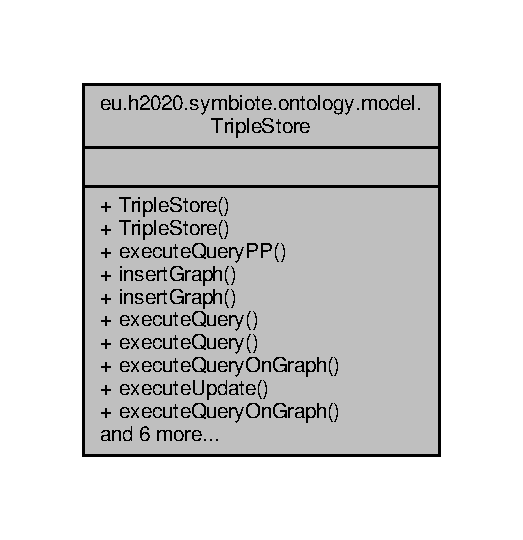
\includegraphics[width=251pt]{classeu_1_1h2020_1_1symbiote_1_1ontology_1_1model_1_1TripleStore__coll__graph}
\end{center}
\end{figure}
\subsection*{Public Member Functions}
\begin{DoxyCompactItemize}
\item 
{\bfseries Triple\+Store} (String directory)\hypertarget{classeu_1_1h2020_1_1symbiote_1_1ontology_1_1model_1_1TripleStore_a625a85b97ad3228d7368b053bea0d399}{}\label{classeu_1_1h2020_1_1symbiote_1_1ontology_1_1model_1_1TripleStore_a625a85b97ad3228d7368b053bea0d399}

\item 
void {\bfseries execute\+Query\+PP} (String query)\hypertarget{classeu_1_1h2020_1_1symbiote_1_1ontology_1_1model_1_1TripleStore_abfcf9b64a71582ef1c37dae8e74902b7}{}\label{classeu_1_1h2020_1_1symbiote_1_1ontology_1_1model_1_1TripleStore_abfcf9b64a71582ef1c37dae8e74902b7}

\item 
void {\bfseries insert\+Graph} (String uri, String rdf, \hyperlink{enumeu_1_1h2020_1_1symbiote_1_1ontology_1_1model_1_1RDFFormat}{R\+D\+F\+Format} format)\hypertarget{classeu_1_1h2020_1_1symbiote_1_1ontology_1_1model_1_1TripleStore_a2564ec9b39ae1c39f540411c04a7a37a}{}\label{classeu_1_1h2020_1_1symbiote_1_1ontology_1_1model_1_1TripleStore_a2564ec9b39ae1c39f540411c04a7a37a}

\item 
void {\bfseries insert\+Graph} (String uri, Model model)\hypertarget{classeu_1_1h2020_1_1symbiote_1_1ontology_1_1model_1_1TripleStore_a29fbdfe06644b181d25e95ce42d6ba53}{}\label{classeu_1_1h2020_1_1symbiote_1_1ontology_1_1model_1_1TripleStore_a29fbdfe06644b181d25e95ce42d6ba53}

\item 
Result\+Set {\bfseries execute\+Query} (String query\+String)\hypertarget{classeu_1_1h2020_1_1symbiote_1_1ontology_1_1model_1_1TripleStore_aa3860b11c0cd7b238742fd291e4573a8}{}\label{classeu_1_1h2020_1_1symbiote_1_1ontology_1_1model_1_1TripleStore_aa3860b11c0cd7b238742fd291e4573a8}

\item 
Result\+Set {\bfseries execute\+Query} (Query query)\hypertarget{classeu_1_1h2020_1_1symbiote_1_1ontology_1_1model_1_1TripleStore_a3854eed46b4772d6d2c32858789d5714}{}\label{classeu_1_1h2020_1_1symbiote_1_1ontology_1_1model_1_1TripleStore_a3854eed46b4772d6d2c32858789d5714}

\item 
Result\+Set {\bfseries execute\+Query\+On\+Graph} (String query\+String, String graph\+Uri)\hypertarget{classeu_1_1h2020_1_1symbiote_1_1ontology_1_1model_1_1TripleStore_a8562e836131eabe86fa017c3de3af0b7}{}\label{classeu_1_1h2020_1_1symbiote_1_1ontology_1_1model_1_1TripleStore_a8562e836131eabe86fa017c3de3af0b7}

\item 
void {\bfseries execute\+Update} (Update\+Request request)\hypertarget{classeu_1_1h2020_1_1symbiote_1_1ontology_1_1model_1_1TripleStore_a8da9fc8adeed9352e6c3b7e858c2dafc}{}\label{classeu_1_1h2020_1_1symbiote_1_1ontology_1_1model_1_1TripleStore_a8da9fc8adeed9352e6c3b7e858c2dafc}

\item 
Result\+Set {\bfseries execute\+Query\+On\+Graph} (Query query, String graph\+Uri)\hypertarget{classeu_1_1h2020_1_1symbiote_1_1ontology_1_1model_1_1TripleStore_a1ab607707674a1e91d45202981719109}{}\label{classeu_1_1h2020_1_1symbiote_1_1ontology_1_1model_1_1TripleStore_a1ab607707674a1e91d45202981719109}

\item 
Model {\bfseries get\+Graph} (String graph)\hypertarget{classeu_1_1h2020_1_1symbiote_1_1ontology_1_1model_1_1TripleStore_a07c5a2fb3c7a67b2c42fb7670c1bd7b7}{}\label{classeu_1_1h2020_1_1symbiote_1_1ontology_1_1model_1_1TripleStore_a07c5a2fb3c7a67b2c42fb7670c1bd7b7}

\item 
Model {\bfseries get\+Default\+Graph} ()\hypertarget{classeu_1_1h2020_1_1symbiote_1_1ontology_1_1model_1_1TripleStore_a30d44c7f131cf2a355ca2432ef0385cf}{}\label{classeu_1_1h2020_1_1symbiote_1_1ontology_1_1model_1_1TripleStore_a30d44c7f131cf2a355ca2432ef0385cf}

\item 
String {\bfseries get\+Graph\+As\+String} (String graph, String syntax)\hypertarget{classeu_1_1h2020_1_1symbiote_1_1ontology_1_1model_1_1TripleStore_a27d54816ac3c52235a954e859064cf03}{}\label{classeu_1_1h2020_1_1symbiote_1_1ontology_1_1model_1_1TripleStore_a27d54816ac3c52235a954e859064cf03}

\item 
List$<$ String $>$ {\bfseries load\+Data\+From\+Dataset} ()\hypertarget{classeu_1_1h2020_1_1symbiote_1_1ontology_1_1model_1_1TripleStore_a40a00ad19248efd65075884b67153e2d}{}\label{classeu_1_1h2020_1_1symbiote_1_1ontology_1_1model_1_1TripleStore_a40a00ad19248efd65075884b67153e2d}

\item 
void {\bfseries print\+Dataset} ()\hypertarget{classeu_1_1h2020_1_1symbiote_1_1ontology_1_1model_1_1TripleStore_a87790ead6163d86afca2a8fef08320d9}{}\label{classeu_1_1h2020_1_1symbiote_1_1ontology_1_1model_1_1TripleStore_a87790ead6163d86afca2a8fef08320d9}

\item 
String {\bfseries get\+Graph\+As\+String} (String graph)\hypertarget{classeu_1_1h2020_1_1symbiote_1_1ontology_1_1model_1_1TripleStore_a89330e0f5789dc40209fa1877a54f783}{}\label{classeu_1_1h2020_1_1symbiote_1_1ontology_1_1model_1_1TripleStore_a89330e0f5789dc40209fa1877a54f783}

\end{DoxyCompactItemize}


\subsection{Detailed Description}
Class representing a triplestore -\/ connected to in-\/memory or disk (T\+DB) jena repository. Creates a spatial index based on Lucene

Contains useful methods to access datastore\+: inserting graphs (save), querying graphs (read).

\begin{DoxyAuthor}{Author}
jab 
\end{DoxyAuthor}


The documentation for this class was generated from the following file\+:\begin{DoxyCompactItemize}
\item 
src/main/java/eu/h2020/symbiote/ontology/model/Triple\+Store.\+java\end{DoxyCompactItemize}

\hypertarget{classeu_1_1h2020_1_1symbiote_1_1query_1_1UpdatePlatformRequestGenerator}{}\section{eu.\+h2020.\+symbiote.\+query.\+Update\+Platform\+Request\+Generator Class Reference}
\label{classeu_1_1h2020_1_1symbiote_1_1query_1_1UpdatePlatformRequestGenerator}\index{eu.\+h2020.\+symbiote.\+query.\+Update\+Platform\+Request\+Generator@{eu.\+h2020.\+symbiote.\+query.\+Update\+Platform\+Request\+Generator}}


Collaboration diagram for eu.\+h2020.\+symbiote.\+query.\+Update\+Platform\+Request\+Generator\+:
\nopagebreak
\begin{figure}[H]
\begin{center}
\leavevmode
\includegraphics[width=259pt]{classeu_1_1h2020_1_1symbiote_1_1query_1_1UpdatePlatformRequestGenerator__coll__graph}
\end{center}
\end{figure}
\subsection*{Public Member Functions}
\begin{DoxyCompactItemize}
\item 
\hyperlink{classeu_1_1h2020_1_1symbiote_1_1query_1_1UpdatePlatformRequestGenerator_a4fb25d7c6e7bff5e8db000400340f9de}{Update\+Platform\+Request\+Generator} (\hyperlink{classeu_1_1h2020_1_1symbiote_1_1model_1_1Platform}{Platform} platform)
\item 
Update\+Request \hyperlink{classeu_1_1h2020_1_1symbiote_1_1query_1_1UpdatePlatformRequestGenerator_a2d2069803f66fd91ab153a856ce0b512}{generate\+Request} ()
\end{DoxyCompactItemize}


\subsection{Detailed Description}
Generator of the update (delete+insert) operation for platforms.

Created by Mael on 26/01/2017. 

\subsection{Constructor \& Destructor Documentation}
\index{eu\+::h2020\+::symbiote\+::query\+::\+Update\+Platform\+Request\+Generator@{eu\+::h2020\+::symbiote\+::query\+::\+Update\+Platform\+Request\+Generator}!Update\+Platform\+Request\+Generator@{Update\+Platform\+Request\+Generator}}
\index{Update\+Platform\+Request\+Generator@{Update\+Platform\+Request\+Generator}!eu\+::h2020\+::symbiote\+::query\+::\+Update\+Platform\+Request\+Generator@{eu\+::h2020\+::symbiote\+::query\+::\+Update\+Platform\+Request\+Generator}}
\subsubsection[{\texorpdfstring{Update\+Platform\+Request\+Generator(\+Platform platform)}{UpdatePlatformRequestGenerator(Platform platform)}}]{\setlength{\rightskip}{0pt plus 5cm}eu.\+h2020.\+symbiote.\+query.\+Update\+Platform\+Request\+Generator.\+Update\+Platform\+Request\+Generator (
\begin{DoxyParamCaption}
\item[{{\bf Platform}}]{platform}
\end{DoxyParamCaption}
)}\hypertarget{classeu_1_1h2020_1_1symbiote_1_1query_1_1UpdatePlatformRequestGenerator_a4fb25d7c6e7bff5e8db000400340f9de}{}\label{classeu_1_1h2020_1_1symbiote_1_1query_1_1UpdatePlatformRequestGenerator_a4fb25d7c6e7bff5e8db000400340f9de}
Constructor of the delete operation. Prepares S\+P\+A\+R\+QL Update statements to delete the platform with specified id and connected statements. To generate the request use \hyperlink{classeu_1_1h2020_1_1symbiote_1_1query_1_1UpdatePlatformRequestGenerator_a2d2069803f66fd91ab153a856ce0b512}{generate\+Request()}.


\begin{DoxyParams}{Parameters}
{\em platform} & Platform containing updated values. \\
\hline
\end{DoxyParams}


\subsection{Member Function Documentation}
\index{eu\+::h2020\+::symbiote\+::query\+::\+Update\+Platform\+Request\+Generator@{eu\+::h2020\+::symbiote\+::query\+::\+Update\+Platform\+Request\+Generator}!generate\+Request@{generate\+Request}}
\index{generate\+Request@{generate\+Request}!eu\+::h2020\+::symbiote\+::query\+::\+Update\+Platform\+Request\+Generator@{eu\+::h2020\+::symbiote\+::query\+::\+Update\+Platform\+Request\+Generator}}
\subsubsection[{\texorpdfstring{generate\+Request()}{generateRequest()}}]{\setlength{\rightskip}{0pt plus 5cm}Update\+Request eu.\+h2020.\+symbiote.\+query.\+Update\+Platform\+Request\+Generator.\+generate\+Request (
\begin{DoxyParamCaption}
{}
\end{DoxyParamCaption}
)}\hypertarget{classeu_1_1h2020_1_1symbiote_1_1query_1_1UpdatePlatformRequestGenerator_a2d2069803f66fd91ab153a856ce0b512}{}\label{classeu_1_1h2020_1_1symbiote_1_1query_1_1UpdatePlatformRequestGenerator_a2d2069803f66fd91ab153a856ce0b512}
Generates the update request, containing delete queries for resource and data linked to the resource.

\begin{DoxyReturn}{Returns}
Update request which allows deletion of the resource and linked information. 
\end{DoxyReturn}


The documentation for this class was generated from the following file\+:\begin{DoxyCompactItemize}
\item 
src/main/java/eu/h2020/symbiote/query/Update\+Platform\+Request\+Generator.\+java\end{DoxyCompactItemize}

%--- End generated contents ---

% Index
\backmatter
\newpage
\phantomsection
\clearemptydoublepage
\addcontentsline{toc}{chapter}{Index}
\printindex

\end{document}
